%!TEX root = ../thesis.tex
\chapter{Diffusion Smoothing Registration of High Resolution Rat Histology} % (fold)
\label{cha:diffusion_smoothing_registration_of_high_resolution_rat_histology}

% If you like chapter abstracts ...
\dblspace
\begin{quote}{\em %!TEX root = ../thesis.tex
Adjacent histological slices can be coregistered accurately and lead to smooth image volumes, owing to their close morphological resemblance and their similar intensity spectra. However, volumes constructed from serial histology registration do not reflect the true 3-dimensional tissue geometry. Registration of histology to a set of coherent reference images yields an authentic geometry on the organ scale, yet the lower resolution and differing modality of the references leads to noisy, jagged volumes on the microstructural scale.

We present in this chapter an algorithm to align neighbouring slices accurately and smoothly without disturbing large scale tissue shape, based on a microscopic model of diffusion. We develop a mathematically sound and general framework of transformational diffusion, based on the Lie theory of continous groups. Using synthetic geometries of cardiac tissue with artificial noise, we demonstrate a robust and precise dispersion of information between slices on a configurable range of scales, recovering volumes which are orders of magnitude smoother and which have maintained faithfully the underlying geometrical signal. We apply the algorithm to the volumes from Chapter~\ref{cha:coregistration_of_high_resolution_rat_histology}, first globally and then again to the region around an epicardial vessel. Previously indiscernible microvasculature and sheet structure become patent. Pericardium and epicardial vessel segmentations show that displacement abberations between adjacent slices of the order of 400$\mu$m are reduced by two orders of magnitude. The methods presented here outperform any such method to reconstruct histological volumes based on reference images currently in the literature. Finally, we discuss several interesting applications and refinements that might be made to the algorithm in specific cases, including anisotropic diffusion based on image features or inter-slice transform magnitudes. The results of this work are presented Computational Methods in Systems Biology 2012 \cite{Gibb2012}, and the work in Chapter~\ref{cha:coregistration_of_high_resolution_rat_histology} and this Chapter will be published in detail in IEEE Transactions on Medical Imaging.
}\end{quote}

\section{Aims} % (fold)
\label{sec:aims}
  We have achieved a reasonable large-scale alignment of the great majority of histological slices to form a consistent tissue volume. Yet we are left with several limitations of the block face technique from Chapter~\ref{cha:coregistration_of_high_resolution_rat_histology}. There is significant underlying noise in the reference images, from the changes in camera position, and the illumination angles and intensities. At 26.6 $\mu$m, the in-plane resolution of the reference images is 24 times coarser than that of the histology slices, precluding an alignment on the scale of cardiac microstructure. Small non-rigid deformations introduced during slicing and rehydration are particular to each slice, and could not be represented fully by the affine registration. Despite obtaining a result that was relatively close to the block face geometry, the overlap of pixel intensities between tissue and wax, and the interslice variability therein, led to a noisy, jagged result that was not always at the global minimum.
    
  \begin{figure}[htbp]
    \centering
    \subfigure[][]{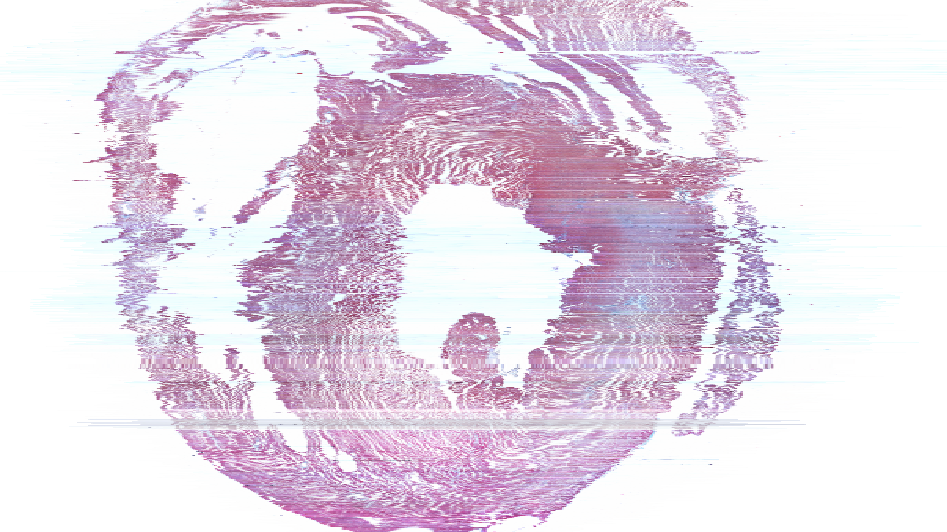
\includegraphics[width=0.9\pagewidth]{Ch6/Figs/banana_0_343}}
    \subfigure[][]{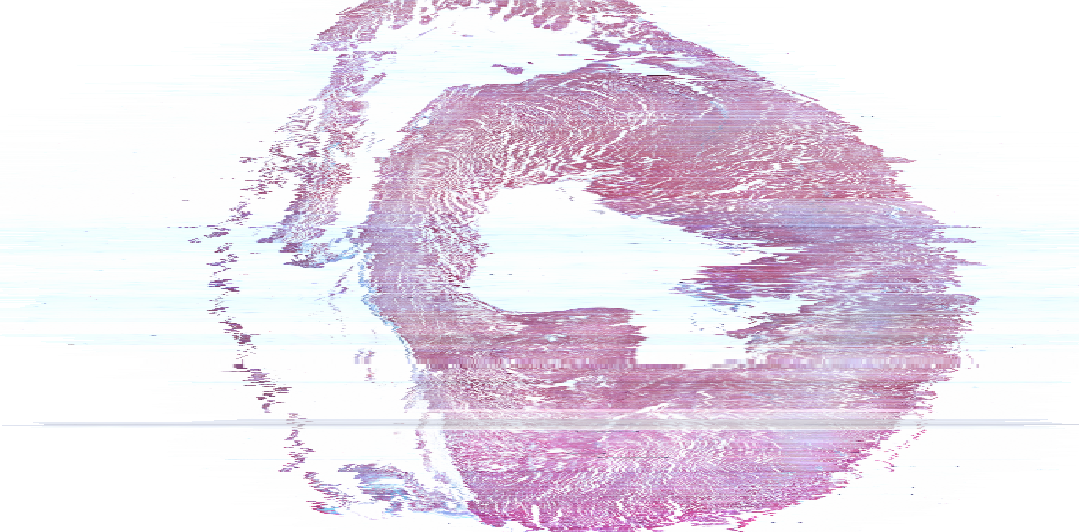
\includegraphics[width=0.9\pagewidth]{Ch6/Figs/banana_1_301}}
    \caption{Cross-sections of the full histological volume, registered using the banana method. As in Figure~\ref{fig:geometric_initialisation}, \textbf{(a)} is perpendicular to the x-axis, and \textbf{(b)} to the y-axis. Even when constrained by a rigid transform, in many areas the slice-to-slice registration is accurate enough that detailed tissue structure is clearly visible. Yet, just as the cylinder does not represent the banana, the resulting geometry of the volume is quite unrelated to ground truth. This is apparent when comparing \textbf{(a)} and \textbf{(b)} to Figure~\ref{fig:LoRes_cross_sections} \textbf{(c)} and \textbf{(d)}, respectively.}
    \label{fig:banana}
  \end{figure}
    
  Adjacent histological images are, in the main, extremely similar in shape, have an extremely similar colour profile and are obtained at the same spatial resolution. These characteristics together make for highly accurate and reliable coregistration. Starting from the first slice in a dataset, previous approaches have registered each successive slice to its predecessor, thus constructing a coherent volume. Figure~\ref{fig:banana} exhibits the application of this method to the rat histology. However, there are several unacceptable characteristics of volumes generated with these techniques. Because each slice is positioned relative to the previous, the displacement due to any single erroneous registration is propagated to every subsequent slice. Furthermore, the volumes suffer from what is known as the `banana problem', stemming from the fact that if a curved banana were sliced evenly and perpendicularly to its length, a volume obtained with a slice-to-slice method would appear straight, having lost the original curvature of the banana. In the case of cardiac histology, volumes approach maximum pairwise symmetry, bearing, if any, a merely coincidental relation to the large-scale geometry of the heart. Finally in this case, only rigid registration may be used, as if the size or shape of slices were unconstrained, every slice would approximate the dimensions of the first, and the heart would approximate a meaty cylinder.
  
  Enter what will be referred to as `transformational diffusion smoothing': a novel technique incorporating the best features from reference-based and slice-to-slice registration methods, and eliminating the weaknesses of both. In this chapter, we will expound its mathematical basis, verify its efficacy over a suite of test geometries, and finally present the much improved histological volumes to which it gives rise.
    
% section aims (end)

\section{Methods} % (fold)
\label{sec:methods}
  This section introduces and details transformational diffusion smoothing in full, in a manner driven by the requirements of the problem at hand. A revision of the theoretical underpinnings of 1-dimensional brownian motion is followed by some simple simulation of diffusion on a discrete grid. In a similar vein, a mathematical exposition of transformational diffusion is followed by its application in several simulated geometries with added artificial affine noise.
  
	\subsection{1D Brownian Diffusion} % (fold)
	\label{sub:a_1d_random_walk_analogy}
	  The central limit theorem states that the mean of a sufficiently large number of independent random variables will be approximately normally distributed, regardless of their individual distribution. Indeed, Einstein's theory of the Brownian motion of a diffusive particle is based on this precept. With this in mind, the simplest model of microscopic diffusion is one in which a particle may move in a random walk in one dimension along the integer number line $\mathbb{Z}$, in steps of either $+1$ or $-1$, with equal probability. Taking each step as an independent random variable $Z_1, Z_2,\ldots$, if the particle's position $S$ starts at $S_0 = 0$, we can express the position of the particle after $N$ steps as
	  \begin{equation}
	    S_N = \sum\limits_{i=1}^N Z_i .
	  \end{equation}
	  The probability of taking $k$ positive steps out of a total of $N$ steps is given by
	  \begin{equation}
	    P(k;N) = \binom{N}{k}\left(\frac{1}{2} \right)^N,
	  \end{equation}
	  where the binomial coefficient
	  \begin{equation}
	    \label{eq:registration:binomial-coefficient}
	     \binom{N}{k} = \frac{N!}{k!(N-k)!},
	  \end{equation}
	  since there are $\binom{N}{k}$ possible ways of taking $k$ and $N - k$ steps of $-1$ and $+1$, respectively. At each independent step, the probability of taking one or the other direction is $\frac{1}{2}$, leading to the product $\frac{1}{2}^N$.
  
	  The de Moivre-Laplace Theorem states that in the limit of large $N$, and in the neighbourhood of $N/2$, the binomial distribution of $k$, and thus of $S_N$, approximates a Gaussian. That is,
    
	  \begin{equation}
	    \label{eq:registration:gaussian-approximation}
	    \binom{N}{k}\left(\frac{1}{2}\right)^N \approx \sqrt{\frac{2}{\pi N}} \
	      e^{-2(k - \frac{N}{2})^2/N}.
	  \end{equation}
    
	  We might consider a concentration of particles $f$ over a discrete 1-dimensional grid $x$, where a proportion $\alpha$ of the particles at each point jump to each of the two neighbouring points per unit time:
    
    \begin{equation}
	    \frac{d f(x, t)}{d t} = \alpha (f(x - \Delta x, t) - 2f(x, t) + f(x + \Delta x, t)).
    \end{equation}
    
    After a small discretised timestep $\Delta t$, and to first order approximation, a proportion $2\alpha \Delta t$ of the particles have taken one step, such that half of them have diffused to the left and half to the right:
  	
	  \begin{gather}
	    \Delta f(x, t + \Delta t) = \alpha \Delta t(f(x - \Delta x, t) - 2f(x, t) + f(x + \Delta x, t)), \\
	    f(x_i, t_{n+1}) = f(x_i, t_n) + \alpha (f(x_{i-1}, t_n) - 2f(x_i, t_n) + f(x_{i+1}, t_n)). \label{eqn:diffusion_1d}
		\end{gather}
  	
	  This diffusion will of course act to smooth and homogenise $f$, since regions of high concentration relative to their neighbours will be reduced, and those of low concentration augmented. It is also clear from (\ref{eq:registration:gaussian-approximation}) that multiple application of this smoothing operation approximates a Gaussian diffusion smoothing.
		
	% subsection a_1d_random_walk_analogy (end)
	
	\subsection{Simulating 1D Diffusion} % (fold)
	\label{sub:simulating_1d_diffusion}
	  \begin{figure}[htbp]
	    \centering
			\subfigure[][0 iterations]{\includegraphics[width=0.4\pagewidth]{Ch6/Figs/1d_noise/alpha_0.40/000}}
			\subfigure[][1 iterations]{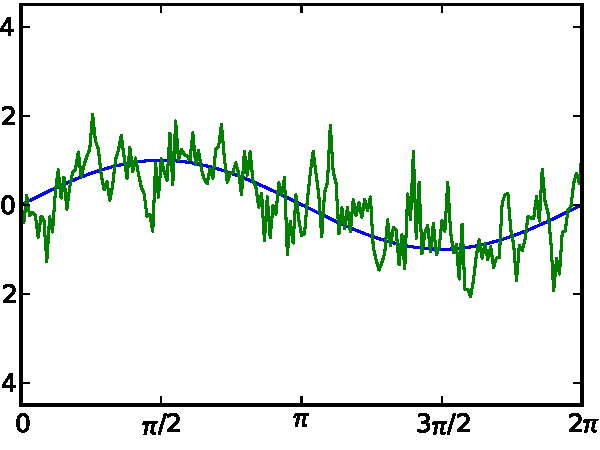
\includegraphics[width=0.4\pagewidth]{Ch6/Figs/1d_noise/alpha_0.40/001}}
			\subfigure[][3 iterations]{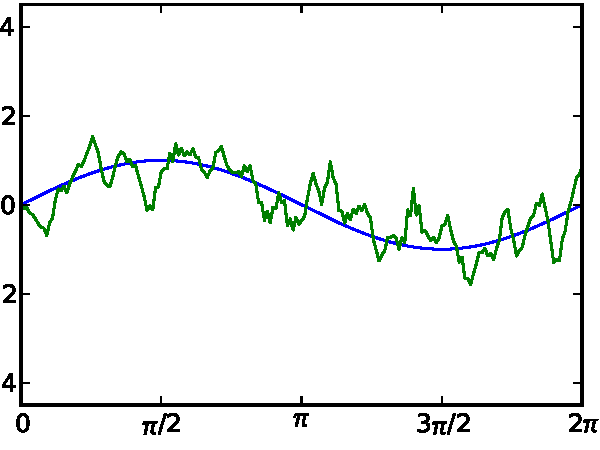
\includegraphics[width=0.4\pagewidth]{Ch6/Figs/1d_noise/alpha_0.40/003}}
			\subfigure[][15 iterations]{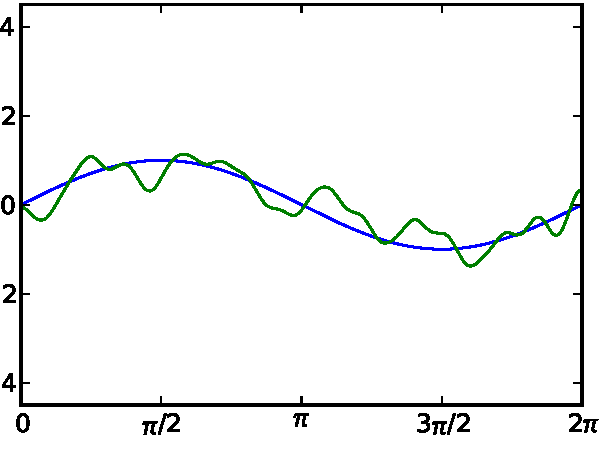
\includegraphics[width=0.4\pagewidth]{Ch6/Figs/1d_noise/alpha_0.40/015}}
			\subfigure[][99 iterations]{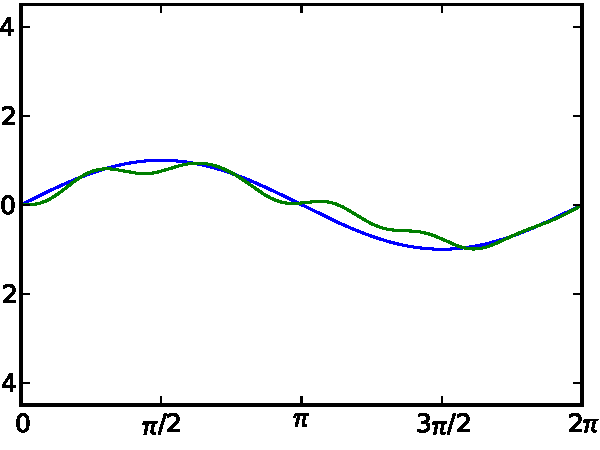
\includegraphics[width=0.4\pagewidth]{Ch6/Figs/1d_noise/alpha_0.40/099}}
			\subfigure[][299 iterations]{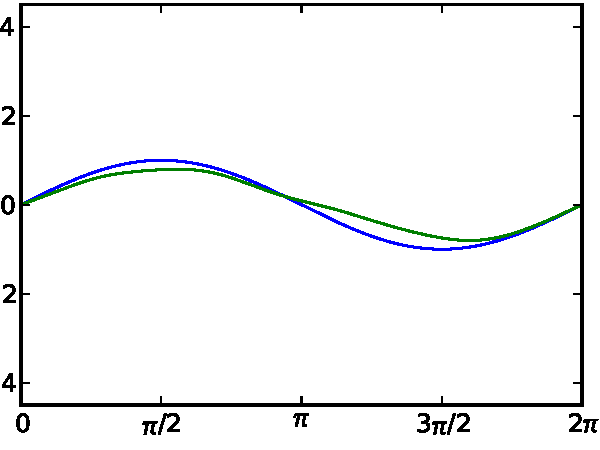
\includegraphics[width=0.4\pagewidth]{Ch6/Figs/1d_noise/alpha_0.40/299}}
	    \caption{A simulation of 1-D diffusion, with $\alpha = 0.4$.}
		  \label{fig:1d_diffusion_0_40}
	  \end{figure}
	
	  \begin{figure}[htbp]
	    \centering
			\subfigure[][0 iterations]{\includegraphics[width=0.4\pagewidth]{Ch6/Figs/1d_noise/alpha_0.49/000}}
			\subfigure[][1 iterations]{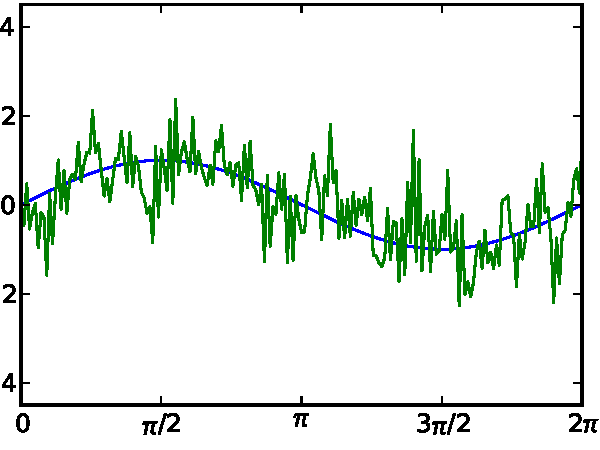
\includegraphics[width=0.4\pagewidth]{Ch6/Figs/1d_noise/alpha_0.49/001}}
			\subfigure[][3 iterations]{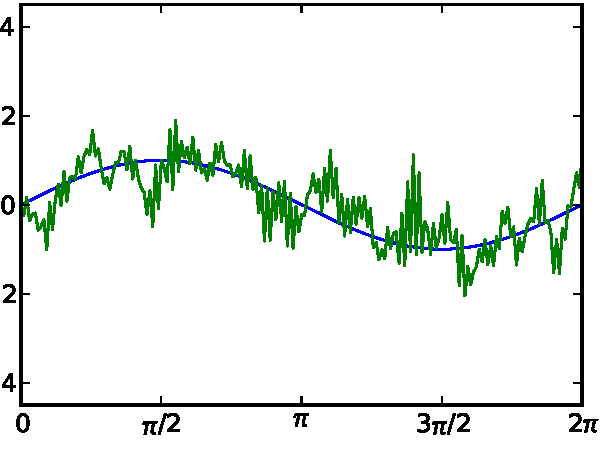
\includegraphics[width=0.4\pagewidth]{Ch6/Figs/1d_noise/alpha_0.49/003}}
			\subfigure[][15 iterations]{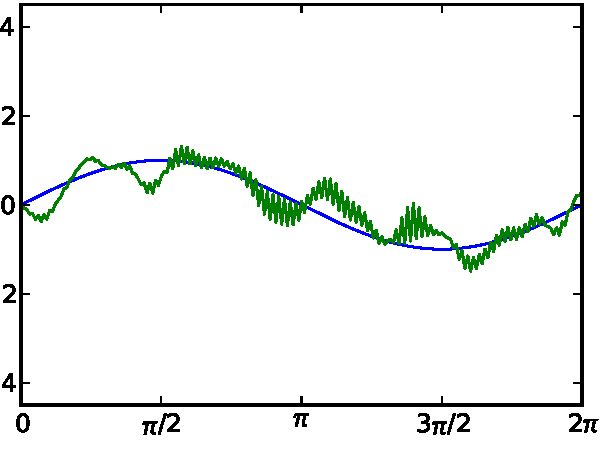
\includegraphics[width=0.4\pagewidth]{Ch6/Figs/1d_noise/alpha_0.49/015}}
			\subfigure[][99 iterations]{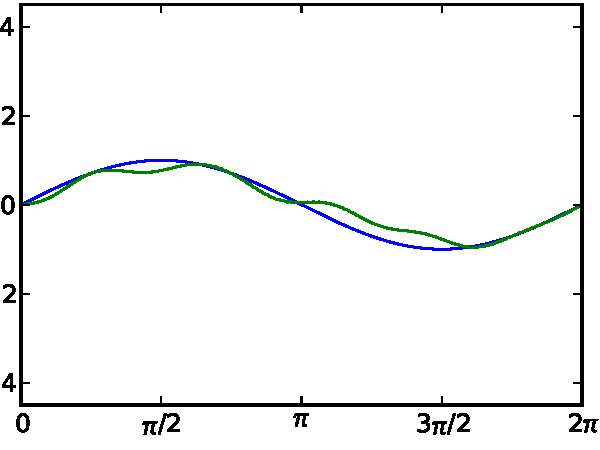
\includegraphics[width=0.4\pagewidth]{Ch6/Figs/1d_noise/alpha_0.49/099}}
			\subfigure[][299 iterations]{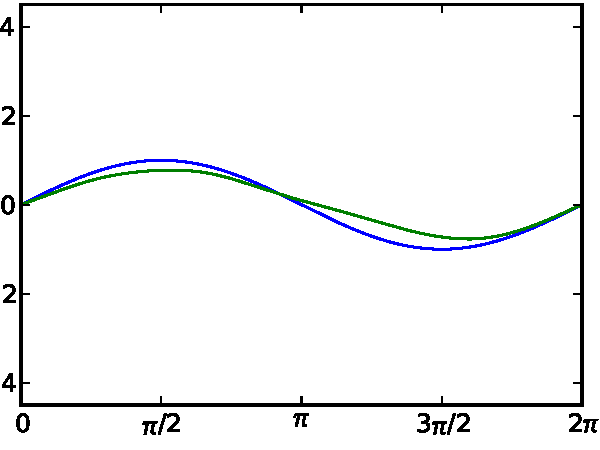
\includegraphics[width=0.4\pagewidth]{Ch6/Figs/1d_noise/alpha_0.49/299}}
	    \caption{A simulation of 1-D diffusion, with $\alpha = 0.49$.}
		  \label{fig:1d_diffusion_0_49}
	  \end{figure}
  
	  \begin{figure}[htbp]
	    \centering
			\subfigure[][0 iterations]{\includegraphics[width=0.4\pagewidth]{Ch6/Figs/1d_noise/alpha_0.50/000}}
			\subfigure[][1 iterations]{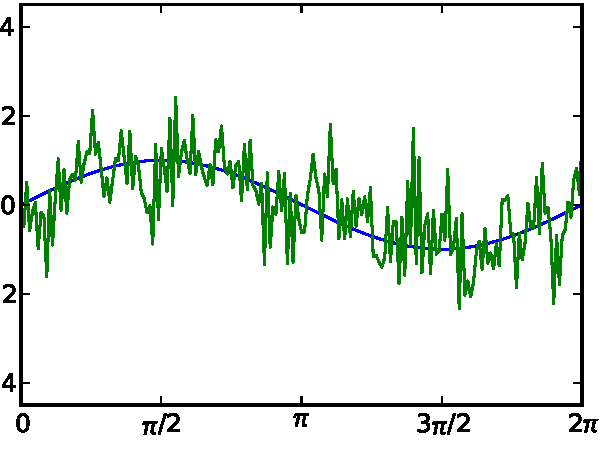
\includegraphics[width=0.4\pagewidth]{Ch6/Figs/1d_noise/alpha_0.50/001}}
			\subfigure[][3 iterations]{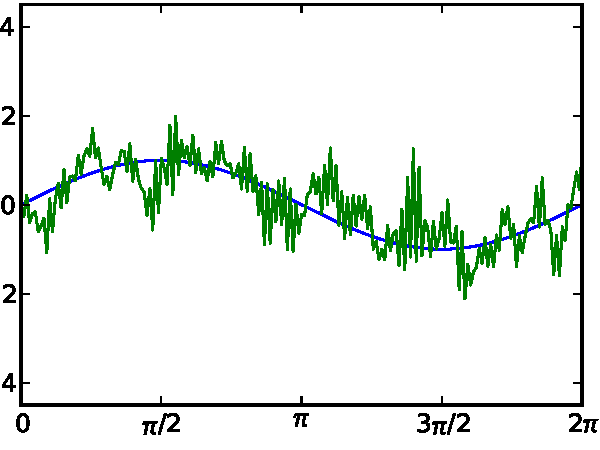
\includegraphics[width=0.4\pagewidth]{Ch6/Figs/1d_noise/alpha_0.50/003}}
			\subfigure[][15 iterations]{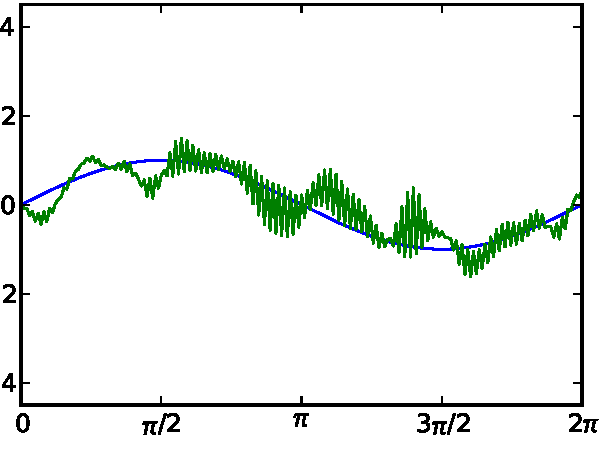
\includegraphics[width=0.4\pagewidth]{Ch6/Figs/1d_noise/alpha_0.50/015}}
			\subfigure[][99 iterations]{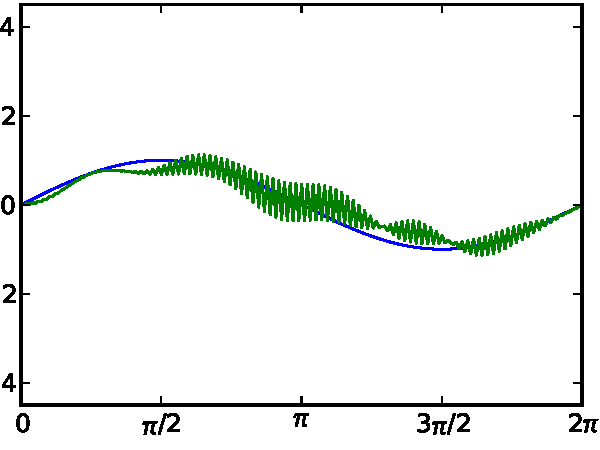
\includegraphics[width=0.4\pagewidth]{Ch6/Figs/1d_noise/alpha_0.50/099}}
			\subfigure[][299 iterations]{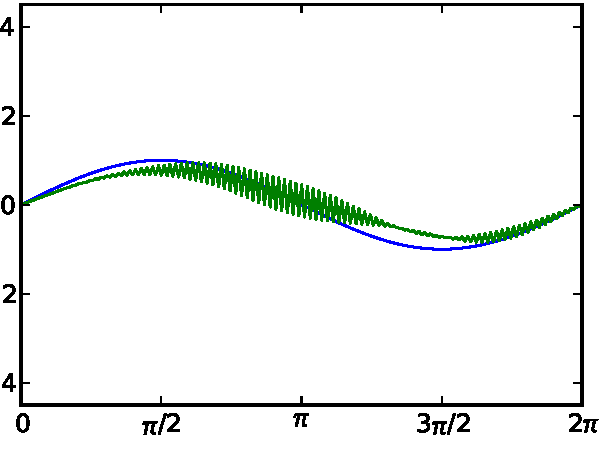
\includegraphics[width=0.4\pagewidth]{Ch6/Figs/1d_noise/alpha_0.50/299}}
	    \caption{A simulation of 1-D diffusion, with $\alpha = 0.5$.}
		  \label{fig:1d_diffusion_0_50}
	  \end{figure}
  
	  \begin{figure}[htbp]
	    \centering
	  	\subfigure[][0 iterations]{\includegraphics[width=0.4\pagewidth]{Ch6/Figs/1d_noise/alpha_0.51/000}}
	  	\subfigure[][1 iterations]{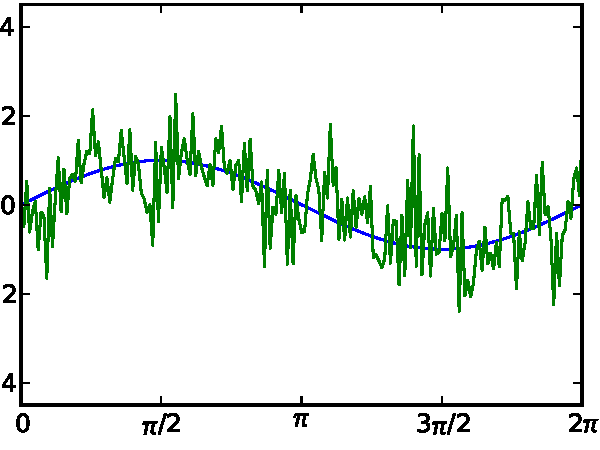
\includegraphics[width=0.4\pagewidth]{Ch6/Figs/1d_noise/alpha_0.51/001}}
	  	\subfigure[][3 iterations]{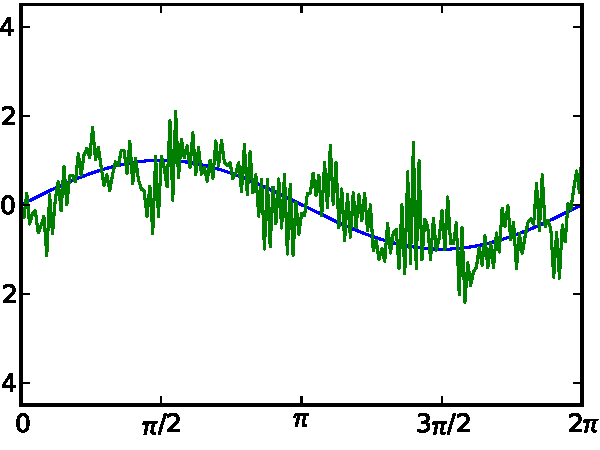
\includegraphics[width=0.4\pagewidth]{Ch6/Figs/1d_noise/alpha_0.51/003}}
	  	\subfigure[][15 iterations]{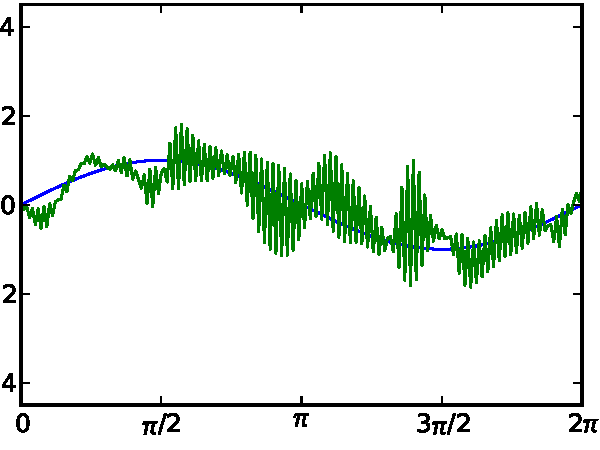
\includegraphics[width=0.4\pagewidth]{Ch6/Figs/1d_noise/alpha_0.51/015}}
	  	\subfigure[][99 iterations]{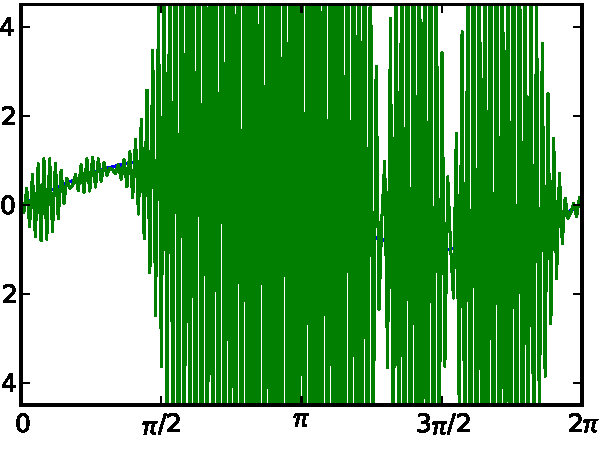
\includegraphics[width=0.4\pagewidth]{Ch6/Figs/1d_noise/alpha_0.51/099}}
	  	\subfigure[][299 iterations]{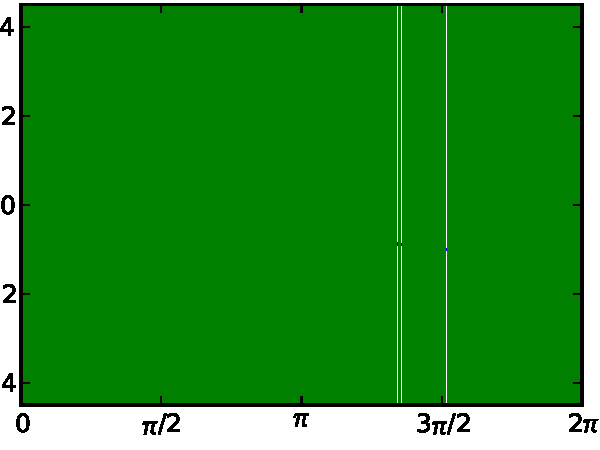
\includegraphics[width=0.4\pagewidth]{Ch6/Figs/1d_noise/alpha_0.51/299}}
	    \caption{A simulation of 1-D diffusion, with $\alpha = 0.51$.}
	    \label{fig:1d_diffusion_0_51}
	  \end{figure}
    
	  
	
	  This process can be simulated quite trivially. A numerical approximation of a sine wave is graphed in blue in each of Figures~\labelcref{fig:1d_diffusion_0_40,fig:1d_diffusion_0_49,fig:1d_diffusion_0_50,fig:1d_diffusion_0_51}, on 200 equispaced points from $0$ to $2\pi$. Random noise from a Gaussian distribution is added, with variance equal to the amplitude of the sine wave, and is plotted in green. The subfigures show the evolution of the noise after 0, 1, 3, 15, 99 and 299 timesteps.
  
	  Our purpose is to smooth out the high frequency random noise from the green wave as quickly and as computationally cheaply as is possible, whilst maintaining the underlying low frequency signal. There is a tradeoff to be made when deciding upon a value for $\alpha$. The greater $\alpha$, the more particles move to the left and right at each iteration, and so the faster the noise is damped. But when $\alpha$ approaches 0.5, almost all of the particles from each bin are moving out at each iteration, and unstable oscillations start to appear. In Figure~\ref{fig:1d_diffusion_0_40}, $\alpha$ is set to 0.4, a great compromise between speed of smoothing and stability. $\alpha$ is set to 0.49 in Figure~\ref{fig:1d_diffusion_0_49}, and the highest frequency is actually damped much more slowly, as oscillatory `swapping' effects start to appear. When $\alpha = 0.5$ in Figure~\ref{fig:1d_diffusion_0_50}, the highest frequency is still undamped after 300 iterations, and by the time $\alpha$ is at 0.51 in Figure~\ref{fig:1d_diffusion_0_51}, the system is unstable. This is not entirely surprising, since it is unphysical for more than all of the particles to diffuse out of a particular bin at each timestep.
	% subsection simulating_1d_diffusion (end)
		
	\subsection{Transformational Diffusion} % (fold)
	\label{sub:transformational_diffusion}
    \subsubsection{Algorithm Overview} % (fold)
    \label{ssub:algorithm_overview}
  	  Our goal is to develop an iterative process that `diffuses' each histological slice image toward its neighbours, in order to smooth out high-frequency transformational noise, whilst maintaining the low-frequency underlying geometry of the volume. An ITK transform $\mathbf{T}$ acting on a point $\mathbf{p}$ maps points in the resampling space to points in the original image space:
		  
  		\begin{equation}
  			\mathbf{p'} = \mathbf{Tp}.
  		\end{equation}
      
  		At iteration $n$ of the proposed process, each slice $i$ in a reconstructed histological stack has associated with it an invertible transform $\mathbf{T}_i^n$. We define the `diffusion transform' $\mathbf{\Delta T}_i^{n,n+1}$, which is formulated to move slice $i$ towards slices $i-1$ and $i+1$, based on the results of registrations between adjacent slices. $\mathbf{\Delta T}_i^{n,n+1}$ is pre-applied to a point in the resampling space of $i$ before $\mathbf{T}_i^n$ to give the adjusted transform $\mathbf{T}_i^{n+1}$, such that
		  
    	\begin{equation}
  			\mathbf{T}_i^{n+1} = \mathbf{T}_i^n \mathbf{\Delta T}_i^{n,n+1}. \label{eqn:adjusted_transforms}
  		\end{equation}
		  
	  How would this $\mathbf{\Delta T}_i^{n,n+1}$ be defined?
		
    % subsubsection algorithm_overview (end)
    
    \subsubsection{Formulating the Diffusion Transforms} % (fold)
    \label{ssub:formulating_the_diffusion_transforms}
      In the case of 1-dimensional diffusion, we can reformulate the right hand side of (\ref{eqn:diffusion_1d}) into two separate terms thusly:
     
	  \begin{align}
	    f(x_i, t_{n+1}) &= f(x_i, t_n) + \alpha ((f(x_{i+1}, t_n) - f(x_i, t_n)) - (f(x_{i-1}, t_n) - f(x_i, t_n)) \\
			\Delta f_i^{n,n+1} &= \alpha (\Delta f_{i,i+1}^n - \Delta f_{i-1,i}^n) \\
			                   &= \alpha \Delta f_{i,i-1}^n + \alpha \Delta f_{i,i+1}^n, \label{eqn:1d_diffusion_operator}
		\end{align}
		
    where $\Delta f_i^{m,n}$ is the difference in $f$ at position $i$ between timestep $m$ and timestep $n$, and $\Delta f_{i,j}^m$ is the difference in $f$ between position $i$ and position $j$ at timestep $m$. From (\ref{eqn:1d_diffusion_operator}), we can see that at each timestep, the concentration at each bin moves towards its left and right neighbour by a proportion $\alpha$ of its difference from each, respectively.
		
	  We might, then, propose analogously that
		
		\begin{equation}
		 	\mathbf{\Delta T}_i^{n,n+1} = \alpha \cdot \mathbf{\Delta T}_{i,i+1}^n \oplus \alpha \cdot \mathbf{\Delta T}_{i,i-1}^n, \label{eqn:transformational_placeholder}
		\end{equation}
	 	
	 	where $\mathbf{\Delta T}_{i,j}^n = (\mathbf{\Delta T}_{j,i}^n)^{-1}$ is defined as the transformation that registers a histological slice $i$ to slice $j$ at iteration $n$, operator $\cdot$ is a placeholder for a binary operator on a scalar and a transform, and operator $\oplus$ is a placeholder for a binary operator on a pair of transforms. We are now equipped to calculate the transforms for progressively smoother and smoother volumes, by first registering each slice to its neighbour to obtain $\mathbf{\Delta T}_{i,i+1}^n$, then computing the diffusion transforms $\mathbf{\Delta T}_i^{n,n+1}$ through \labelcref{eqn:transformational_placeholder}, and finally applying them to the original transforms through \labelcref{eqn:adjusted_transforms} to obtain $\mathbf{T}_i^{n+1}$. The question now emerges: what precise form do the two binary operators take? We will start by outlining their desirable properties, and then discuss implementations that satisfy these constraints.
    % subsubsection formulating_the_diffusion_transforms (end)
		
    \subsubsection{Formulating the Transform Operators} % (fold)
    \label{ssub:formulating_the_transform_operators}
		The operator $\cdot$ takes two operands: a scalar and a transform. We would like $0$ to be the null operand on $\mathbf{T}$, so that when $\alpha = 0$, no diffusion occurs. We would like $1$ to be the identity operand on $\mathbf{T}$, so that when $\alpha = 1$, the transform from each term in (\ref{eqn:transformational_placeholder}) would diffuse the slice exactly to the position of its equivalent neighbour. Ideally, we would also like addition of the scalar operand to distribute over the serial application of the resultant transforms, so that transforms vary smoothly and naturally with respect to the scalar operand. This final condition can be satisfied for certain transforms, such as linear transforms and vector field transforms, but cannot be satisfied in general for others, such as b-spline transforms. To summarise in mathematical form, we would like the following to hold:
		
		\begin{gather}
			0 \cdot \mathbf{T} = \mathbf{I} \label{eqn:null} \\
			1 \cdot \mathbf{T} = \mathbf{T} \label{eqn:identity} \\
			(\alpha \cdot \mathbf{T}) (\beta \cdot \mathbf{T}) = (\alpha + \beta) \cdot \mathbf{T} \label{eqn:distributivity}
		\end{gather}
	 	
	  The operator $\oplus$ takes two transform operands. Commutativity must hold if the diffusion is to be symmetric i.e. behave identically if the order of the slices is reversed. If statistics are to be calculated on more than two transformations, it is also necessary for associativity to hold, so that the order of application of operator $\oplus$ is not preferential to any subset of transform operands. That is,
		
		\begin{gather}
			\forall \mathbf{S}, \mathbf{T} : \mathbf{S} \oplus \mathbf{T} = \mathbf{T} \oplus \mathbf{S} \label{eqn:commutativity} \\
			\forall \mathbf{S}, \mathbf{T} : (\mathbf{S} \oplus \mathbf{T}) \oplus \mathbf{U} = \mathbf{S} \oplus (\mathbf{T} \oplus \mathbf{U}). \label{eqn:associativity}
		\end{gather}
		
		Unfortunately, commutativity rules out the straightforward serial application of transforms. For example, in the general case of matrix multiplication, $AB \ne BA$. One solution is to use the transform that is equivalent to returning the Euclidian midpoint of $\mathbf{Sp}$ and $\mathbf{Tp}$ for all $\mathbf{p}$. However, the result may not always be representable by some types of transform (notably b-spline transforms), and further, it may be dependent on the order that the $\oplus$ operator is applied. In group theoretical terms, two axioms of the group $(\mathbf{T},\oplus)$ are violated: closure and associativity. Aside from anything else, the Euclidian midpoint approach leads in many cases to unnatural results, such as the `bulging' effect noted in \cite{Arsigny2005a}, and the null matrix in 2D between transforms separated by a rotation of $\pi$.
        
        In the case of rotation matrices, it seems sensible to return the sum of the two angles; and for similarity transforms, the product of the two enlargement factors. Inductively therefore, the operator $\oplus$ would do well to return the summation of some appropriate parameterisation of the operand transforms. The challenge is set to find that parameterisation.
		
	  It is elucidating to consider the general mathematical form constrained by \labelcref{eqn:null,eqn:identity,eqn:distributivity,eqn:commutativity,eqn:distributivity} applied to concrete classes of transform, in order of increasing complexity: translation transforms, rotation transforms, similarity transforms, affine transforms and more general deformable transforms. An ITK affine transform $\mathbf{T}$ acting on a point $\mathbf{p}$ consists of a matrix transformation $\mathbf{M}$, followed by a translation by an offset vector $\mathbf{o}$:
		
		\begin{equation}
			\mathbf{p'} = \mathbf{Tp}= \mathbf{Mp} + \mathbf{o}.
		\end{equation}
		
		In the simplest case of translation transforms, where $\mathbf{M}$ is the identity matrix $\mathbf{I}$ i.e. $\mathbf{Tp} = \mathbf{p} + \mathbf{o}$, the two translation parameters are independent and individually identical to the 1-dimensional diffusion in (\ref{eqn:1d_diffusion_operator}). Operator $\cdot$ is a scalar multiplication of each offset parameter, and operator $\oplus$ is the commutative serial application of the transforms (or equivalently, addition of the respective parameters):
		
		\begin{align}
			(\alpha \cdot \mathbf{T}) \mathbf{p} &= \mathbf{p} + \alpha\mathbf{o} \label{eqn:translation_cdot}\\
			(\mathbf{S} \oplus \mathbf{T}) \mathbf{p} &= \mathbf{STp} \\
			                                          &= \mathbf{p} + \mathbf{o_S} + \mathbf{o_T} \label{eqn:translation_oplus}
		\end{align}
		
		Clearly, these two operators satisfy \labelcref{eqn:null,eqn:identity,eqn:distributivity,eqn:commutativity,eqn:associativity}. (\ref{eqn:transformational_placeholder}) becomes
		
		\begin{align}
		 	\mathbf{\Delta T}_i^{n,n+1} \mathbf{p} &= (\alpha \mathbf{\Delta T}_{i,i-1}^n) (\alpha \mathbf{\Delta T}_{i,i+1}^n) \mathbf{p} \\
			\mathbf{p} + \mathbf{o}_i^{n,n+1} &= \mathbf{p} + \alpha \mathbf{o}_{i,i-1}^n + \alpha \mathbf{o}_{i,i+1}^n \\
			\mathbf{o}_i^{n,n+1} &= \alpha (\mathbf{o}_{i,i-1}^n + \mathbf{o}_{i,i+1}^n) 
		\end{align}
		
		The offsets are therefore trivially analogous to (\ref{eqn:1d_diffusion_operator}).
		
		In the case of rigid transforms, $\mathbf{M}$ is a rotation matrix
		
		\begin{equation}
			\mathbf{R}(\theta) = \left( \begin{matrix}
			  										 \cos \theta & -\sin\theta \\
														 \sin\theta & \cos\theta
					                 \end{matrix} \right) .
		\end{equation}
		
		In 2 dimensions, rotation matrices commute, and the result of their multiplication is simply a rotation matrix with angle equal to the sum of the operands' angles; in the special case where there are no offsets, then serial application of the transforms is a candidate for operator $\oplus$ according to (\ref{eqn:commutativity}):
		
		\begin{equation}
			\mathbf{S} \oplus \mathbf{T} = \mathbf{R}(\theta_\mathbf{S})\mathbf{R}(\theta_\mathbf{T}) = \mathbf{R}(\theta_\mathbf{S} + \theta_\mathbf{T}) = \mathbf{T} \oplus \mathbf{S}
		\end{equation}
		
		
		In a similar vein, an operator $\cdot$ that multiplies the angle of the input transform with $\alpha$ fulfils criteria \labelcref{eqn:null,eqn:identity,eqn:distributivity}:
    
    \begin{equation}
      \alpha \cdot \mathbf{T} = \mathbf{R}(\alpha\theta).
    \end{equation}
		
        In the case of similarity transforms with no offset, $\mathbf{M}$ is a rotation matrix $\mathbf{R}$ multiplied by an enlargement $\sigma$:
        
        \begin{equation}
            \mathbf{T} = \sigma\mathbf{R}(\theta).
        \end{equation}
        
        Since scalar multiplications commute with matrix transformations, if the operator $\cdot$ is constructed to scale geometrically, the situation is very similar to that of rotation matrices and \labelcref{eqn:null,eqn:identity,eqn:distributivity,eqn:commutativity,eqn:associativity} still apply:
        
        \begin{gather}
            \alpha \cdot \mathbf{T} = \sigma^{\alpha}\mathbf{R}(\alpha\theta) \\
            (\alpha \cdot \mathbf{T})(\beta \cdot \mathbf{T}) = \sigma^{\alpha + \beta}\mathbf{R}((\alpha + \beta)\theta) = (\alpha + \beta) \cdot \mathbf{T} \\
			\mathbf{S} \oplus \mathbf{T} = \sigma_\mathbf{S}\mathbf{R}(\theta_\mathbf{S})\sigma_\mathbf{T}\mathbf{R}(\theta_\mathbf{T}) = \sigma_\mathbf{S}\sigma_\mathbf{T}\mathbf{R}(\theta_\mathbf{S} + \theta_\mathbf{T}) = \mathbf{T} \oplus \mathbf{S} \\
			(\mathbf{S} \oplus \mathbf{T}) \oplus \mathbf{U} = \sigma_\mathbf{S}\sigma_\mathbf{T}\sigma_\mathbf{U}\mathbf{R}(\theta_\mathbf{S} + \theta_\mathbf{T} + \theta_\mathbf{U}) = \mathbf{S} \oplus (\mathbf{T} \oplus \mathbf{U}).
        \end{gather}
		
		In the more general case of diagonalisable affine matrix transformations, in the absence of translations, and when $\mathbf{S}$ and $\mathbf{T}$ can be diagonalised by the same matrix $\mathbf{V}$ i.e. $\mathbf{S} = \mathbf{VD_SV}^{-1}$ and $\mathbf{T} = \mathbf{VD_TV}^{-1}$, commutativity still holds for serial application:
        
        \begin{equation}
			\mathbf{S} \oplus \mathbf{T} = \mathbf{ST} = \mathbf{VD_SV}^{-1}\mathbf{VD_TV}^{-1} = \mathbf{VD_SD_TV}^{-1} =\mathbf{VD_TD_SV}^{-1} = \mathbf{T} \oplus \mathbf{S},
        \end{equation}
        
        with associativity of course holding for the serial application of affine transformations in general. However, when $\mathbf{M_S}$ and $\mathbf{M_T}$ no longer commute, serial application of transforms is no longer sufficient. There is also no obvious form of operator $\cdot$ which satisfies \labelcref{eqn:null,eqn:identity,eqn:distributivity}. We must take recourse to a more general formulation of operators $\cdot$ and $\oplus$.
        
        It is here that we must introduce the concept of the matrix exponential:
        
        \begin{equation}
          e^{\mathbf{M}} = \sum_{k=0}^{\infty}\frac{1}{k!}\mathbf{M}^k. \label{eqn:matrix_exponential}
        \end{equation}
        
        Conversely, a logarithm $\mathbf{L}$ of a matrix $\mathbf{M}$ is another matrix such that $e^\mathbf{L} = \mathbf{M}$. For any invertible matrix $\mathbf{Y}$, it is clear that
        
        \begin{gather}
          (\mathbf{YM}\mathbf{Y}^{-1})^n = \mathbf{Y}\mathbf{M}^n\mathbf{Y}^{-1}, n \in \mathbb{N}.
        \end{gather}
        
        It then follows from (\ref{eqn:matrix_exponential}) that
        
        \begin{align}
          \mathbf{Y}e^{\mathbf{M}}\mathbf{Y}^{-1} &= \mathbf{Y}\left(\sum_{k=0}^{\infty}\frac{1}{k!}\mathbf{M}^k\right)\mathbf{Y}^{-1} \\
                                                  &= \sum_{k=0}^{\infty}\frac{1}{k!}\mathbf{Y}\mathbf{M}^k\mathbf{Y}^{-1} \\
                                                  &= \sum_{k=0}^{\infty}\frac{1}{k!}(\mathbf{YM}\mathbf{Y}^{-1})^k \label{eqn:diagonal_exp} \\
                                                  &= e^{\mathbf{YM}\mathbf{Y}^{-1}}.
        \end{align}
        
        If $\mathbf{M}$ is diagonalisable, and we choose a $\mathbf{Y}$ that diagonalises $\mathbf{M}$, such that $\mathbf{D} = \mathbf{YMY}^{-1}$, (\ref{eqn:diagonal_exp}) becomes trivially analogous to the Taylor expansion for a scalar exponential, and we can then simply compute the exponential of each diagonal element of $\mathbf{D}$. It follows that the logarithm of a positive definite diagonal matrix can be computed by taking the logarithm of each of its elements.
        
        It turns out that when a matrix $\mathbf{M}$ has a logarithm $\mathbf{L}$, $\mathbf{M}$ is in a Lie group --- a group on a smooth manifold. $\mathbf{L}$ is the corresponding element of the associated Lie algebra. $\mathbf{L}$ is an `infinitessimal generator', and its value determines the tangent space at the identity $\mathbf{I}$. Informally, this means that there exists a matrix $\mathbf{I} + \epsilon \mathbf{L}$ that is extremely close to the identity, such that when applied repeatedly an extremely large number of times i.e. $(\mathbf{I} + \epsilon \mathbf{L})^n$, the result eventually becomes $\mathbf{M}$.
        
        If we define operator $\cdot$ in terms of the exponential and the logarithm of $\mathbf{M}$, \labelcref{eqn:null,eqn:identity,eqn:distributivity} are all satisfied:
        
        \begin{gather}
          \alpha \cdot \mathbf{M} = e^{\alpha\ln\mathbf{M}} \\
          0 \cdot \mathbf{M} = e^0 = \mathbf{I} \\
          1 \cdot \mathbf{M} = e^{\ln\mathbf{M}} = \mathbf{M} \\
          (\alpha \cdot \mathbf{M})(\beta \cdot \mathbf{M}) = e^{\alpha\ln\mathbf{M}}e^{\beta\ln\mathbf{M}}
                                                            = e^{(\alpha + \beta)\ln\mathbf{M}}
                                                            = (\alpha + \beta) \cdot \mathbf{M}.
        \end{gather}
        
        We can define operator $\oplus$ as a simple addition of the matrix logarithms in log-Euclidian space, followed by a mapping back to transform space with the exponential operator:
        
        \begin{equation}
          \mathbf{M_S} \oplus \mathbf{M_T} = e^{\ln\mathbf{M_S} + \ln\mathbf{M_T}}.
        \end{equation}
        
        Because all operations are homomorphic with Euclidian vector space, this operator always fulfils the commutativity and associativity criteria
        
        \begin{gather}
          \mathbf{M_S} \oplus \mathbf{M_T} = e^{\ln\mathbf{M_S} + \ln\mathbf{M_T}} = \mathbf{M_T} \oplus \mathbf{M_S} \\
          (\mathbf{M_S}\oplus\mathbf{M_T})\oplus\mathbf{M_U} = e^{\ln\mathbf{M_S} + \ln\mathbf{M_T} + \ln\mathbf{M_U}} = \mathbf{M_S}\oplus(\mathbf{M_T}\oplus\mathbf{M_U}).
        \end{gather}
        
        It is pleasing to note that this new formula coincides with the special cases of rotation, similarity and diagonalisability discussed previously, since whenever the two matrices commute,
        
        \begin{equation}
          \mathbf{M_SM_T} = e^{\ln\mathbf{M_S}}e^{\ln\mathbf{M_T}} = e^{\ln\mathbf{M_S} + \ln\mathbf{M_T}} = \mathbf{M_S} \oplus \mathbf{M_T}.
        \end{equation}
        
        This `log-Euclidian' approach is expounded with Titanic mathematical rigour in \cite{Arsigny2005,Arsigny2005a,Pennec2006}, based on work in \cite{Pennec2006a}. However, being motivated by the interpolation of MRI data, the treatise is limited to tensors; that is, symmetric matrices with no translation.
        
		    So far, the discussion has been limited to cases with zero offset. When offsets are introduced, even when their respective matrices commute, the commutativity of transforms in (\ref{eqn:commutativity}) no longer holds when serial action akin to (\ref{eqn:translation_oplus}) is introduced na\"ively:
		    
        \begin{equation}
          (\mathbf{S} \oplus \mathbf{T})\mathbf{p} = (\mathbf{M_S} \oplus \mathbf{M_T})\mathbf{p} + \mathbf{M_So_T} + \mathbf{o_S} \ne (\mathbf{T} \oplus \mathbf{S})\mathbf{p}.
        \end{equation}
        
        If commutivity is forced, by averaging the offset contributions from both permutations of the operands i.e.
        
        \begin{equation}
          (\mathbf{S} \oplus \mathbf{T})\mathbf{p} = (\mathbf{T} \oplus \mathbf{S})\mathbf{p} = (\mathbf{M_S} \oplus \mathbf{M_T})\mathbf{p} + \frac{1}{2}\left(\left( \mathbf{M_S} + \mathbf{I} \right) \mathbf{o_T} + \left( \mathbf{M_T} + \mathbf{I} \right)\mathbf{o_S}\right),
        \end{equation}

        then associativity breaks down. The same underlying structure precludes a linear interpolation in operator $\cdot$ akin to \labelcref{eqn:translation_cdot} in the presence of a non-identical matrix:
        
        \begin{gather}
          (\alpha \cdot \mathbf{T})(\beta \cdot \mathbf{T})\mathbf{p} = \mathbf{M}_{\alpha+\beta}\mathbf{p} + \beta\mathbf{M}_{\alpha}\mathbf{o} + \alpha\mathbf{o} \ne (\alpha + \beta) \cdot \mathbf{T}.
        \end{gather}
        
        When $\mathbf{I} - \mathbf{M}$ is invertible --- that is, when none of the eigenvalues of $\mathbf{M}$ are equal to 1 --- we can express a transform as a matrix transformation about a single invariant centre, with no offset:
        
        \begin{gather}
          \mathbf{Tp} = \mathbf{Mp} + \mathbf{o} = \mathbf{M}(\mathbf{p}-\mathbf{c}) + \mathbf{c} \\
          \mathbf{o} = (\mathbf{I} - \mathbf{M})\mathbf{c} \\
          \mathbf{c} = (\mathbf{I} - \mathbf{M})^{-1}\mathbf{o}.
        \end{gather}
        
        We can then reformulate operator $\cdot$ as a log-Euclidian transformation about this invariant centre and satisfy distributivity:
        
        \begin{gather}
          \alpha \cdot \mathbf{T} = e^{\alpha\ln\mathbf{M}}(p - c) + c \label{eqn:affine_cdot} \\
          \begin{split}
            (\alpha \cdot \mathbf{T})(\beta \cdot \mathbf{T}) &= e^{\alpha\ln\mathbf{M}}((e^{\beta\ln\mathbf{M}}(p - c) + c) - c) + c \\
                                                              &= e^{\alpha\ln\mathbf{M}}(e^{\beta\ln\mathbf{M}}(p - c)) + c \\
                                                              &= e^{(\alpha + \beta)\ln\mathbf{M}}(p - c) + c \\
                                                              &= (\alpha + \beta) \cdot \mathbf{T}.
          \end{split}
        \end{gather}
        
        With this condition satisfied, $\alpha\cdot\mathbf{T}$ is equivalent to $\mathbf{T}^{\alpha}$. In order to derive the common centre of the two operands of operator $\oplus$, let us consider the infinitesimal case
        
        \begin{gather}
          \delta \cdot \mathbf{U} = (\delta \cdot \mathbf{S}) \oplus (\delta \cdot \mathbf{T}) \approx (\delta \cdot \mathbf{S}) (\delta \cdot \mathbf{T}) \\
          \begin{split}
            e^{\delta(\ln \mathbf{M_S} + \ln \mathbf{M_T})}\mathbf{p} + (\mathbf{I} - e^{\delta(\ln \mathbf{M_S} + \ln \mathbf{M_T})})\mathbf{c_U} =
              &e^{\delta \ln \mathbf{M_S}}e^{\delta \ln \mathbf{M_T}}\mathbf{p} \\
              &+ e^{\delta \ln \mathbf{M_S}}(\mathbf{I} - e^{\delta \ln \mathbf{T}})\mathbf{c_T} \\
              &+ (\mathbf{I} - e^{\delta \ln \mathbf{M_S}})\mathbf{c_S}. \label{eqn:infinitesimal_oplus}
          \end{split}
        \end{gather}
        
        We can see from the series in (\ref{eqn:matrix_exponential}) that
        
        \begin{equation}
          e^{\delta \ln \mathbf{M}} = \mathbf{I} + \delta \ln \mathbf{M} + \mathcal{O}((\delta \ln \mathbf{M})^2).
        \end{equation}
        
        Applying this to (\ref{eqn:infinitesimal_oplus}), we obtain
        
        \begin{equation}
          (\ln\mathbf{M_S} + \ln\mathbf{M_T})\mathbf{c_U} = (\ln\mathbf{M_S})\mathbf{c_S} + (\ln\mathbf{M_T})\mathbf{c_T}.
        \end{equation}
        
        The general form of operator $\oplus$ is then finally
        
        \begin{gather}
          \mathbf{S} \oplus \mathbf{T} = e^{\ln\mathbf{M_S} + \ln\mathbf{M_T}}(\mathbf{p} - \mathbf{c}) + \mathbf{c}, \nonumber \\
          \mathbf{c} = (\ln\mathbf{M_S} + \ln\mathbf{M_T})^{-1}((\ln\mathbf{M_S})\mathbf{c_S} + (\ln\mathbf{M_T})\mathbf{c_T}). \label{eqn:affine_oplus}
        \end{gather}
        
        Commutativity is evident by inspection, and associativity is simply demonstrated:
        
        \begin{gather}
          \begin{split}
            (\mathbf{S} \oplus \mathbf{T}) \oplus \mathbf{U} &= \exp(\ln(e^{\ln\mathbf{M_S} + \ln\mathbf{M_T}}) + \ln\mathbf{M_U})(\mathbf{p} - \mathbf{c}) + \mathbf{c} \\
                                                             &= e^{\ln\mathbf{M_S} + \ln\mathbf{M_T} + \ln\mathbf{M_U}}(\mathbf{p} - \mathbf{c}) + \mathbf{c},
          \end{split} \\
          \begin{split}
            \mathbf{c} &= (\ln\mathbf{M_{S \oplus T}} + \ln\mathbf{M_U})^{-1}((\ln\mathbf{M_{S \oplus T}})\mathbf{c_{S \oplus T}} + (\ln\mathbf{M_U})\mathbf{c_U}) \\
                       &= (\ln\mathbf{M_S} + \ln\mathbf{M_T} + \ln\mathbf{M_U})^{-1}((\ln\mathbf{M_S})\mathbf{c_S} + (\ln\mathbf{M_T})\mathbf{c_T} + (\ln\mathbf{M_U})\mathbf{c_U}).
          \end{split}
        \end{gather}
        
        As a last algebraic-structural perk, it can be shown from \labelcref{eqn:affine_cdot,eqn:affine_oplus} that the operation of $\cdot$ by a scalar distributes over the operation of $\oplus$ on two affine transformations. In particular,
        
        \begin{equation}
          (\alpha \cdot \mathbf{S}) \oplus (\alpha \cdot \mathbf{T}) = \alpha \cdot (\mathbf{S} \oplus \mathbf{T}).
        \end{equation}
        
        In the case where $\mathbf{M} - \mathbf{I}$ is singular and there is no central invariate coordinate along the singular dimensions, it is of course natural that operator $\cdot$ interpolates the translation coordinates linearly along those dimensions as in (\ref{eqn:translation_cdot}), and that operator $\oplus$ sums translations arithmetically as in (\ref{eqn:translation_oplus}).
        
        A similar Lie theoretical approach must be taken when implementing operators $\cdot$ and $\oplus$ for more general non-rigid transforms, such as displacement field transforms. However, any differentiable transform will approximate an affine transformation at scales smaller than its curvature, and the implementations expounded here will suffice to smooth out those smaller subregions.
    % subsubsection formulating_the_transform_operators (end)
	% subsection transformational_diffusion (end)
	
  \subsection{Simulating Transformational Diffusion} % (fold)
  \label{sub:simulating_transformational_diffusion}
  
  In order to test the efficacy of the algorithm in a quantitative way, it was necessary to devise several test geometries. Four stacks of 200 identical slices were constructed: one straight column with identical transforms for each slice; one column with sinusoidal, snake-like translation added; one column with sinusoidal rotation added; and one column incorporating both a translational and a rotational signal. The transform parameters of each slice were then perturbed by random Gaussian noise, with $\sigma$ equal to the amplitude of the translational and rotational signal, respectively.
  
  % colour slice differences
  \begin{figure}[htbp]
    \centering
    \subfigure[][unperturbed image]{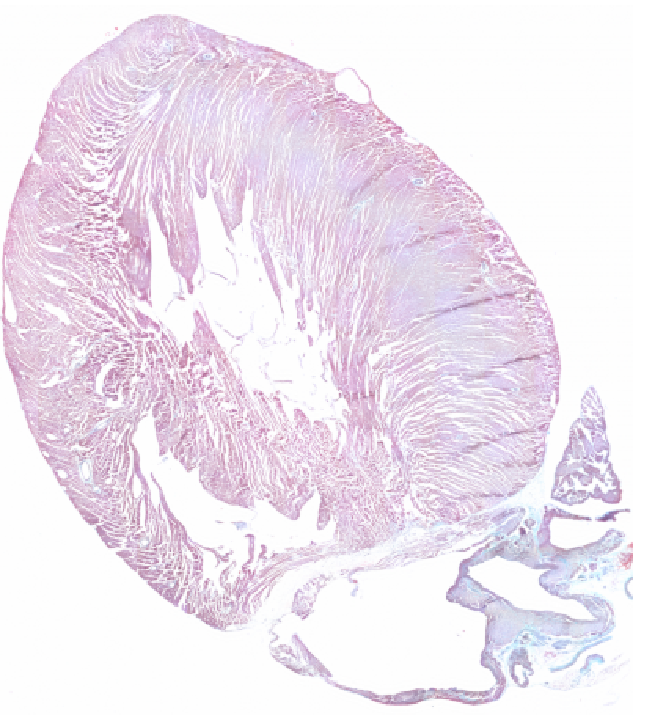
\includegraphics[height=0.365\textheight,type=pdf,ext=.pdf,read=.pdf]{Ch6/Figs/dummies/colour_perfect_slice}} \quad
    \subfigure[][image with transformational noise]{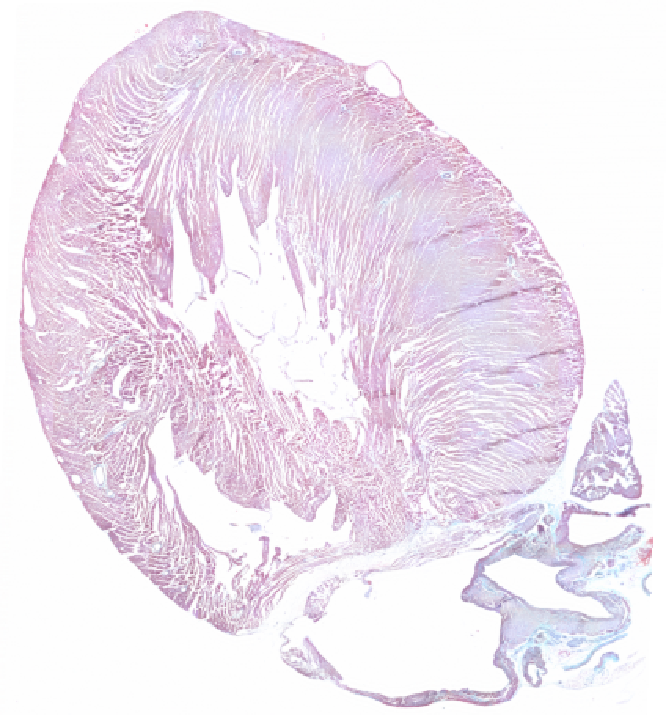
\includegraphics[height=0.365\textheight,type=pdf,ext=.pdf,read=.pdf]{Ch6/Figs/dummies/colour_noisy_slice}} \\
    \subfigure[][Red-blue channels of intensities]{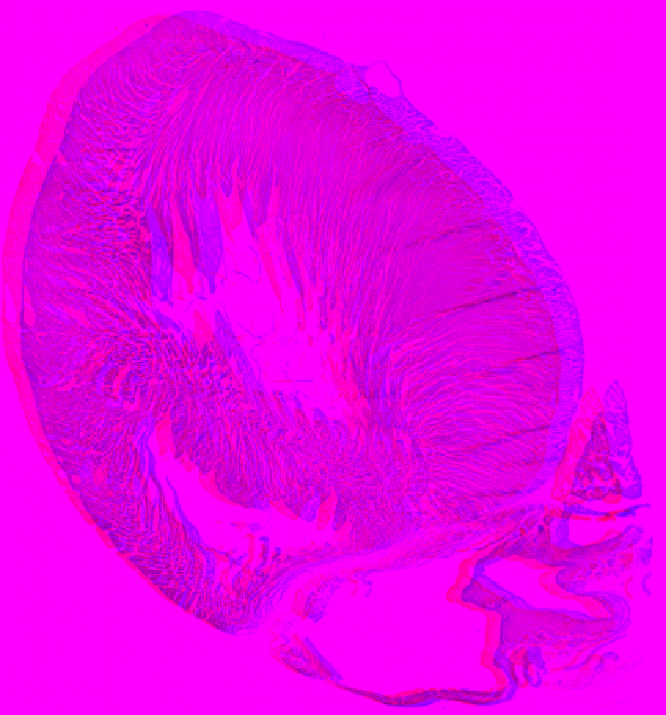
\includegraphics[height=0.365\textheight,type=pdf,ext=.pdf,read=.pdf]{Ch6/Figs/dummies/colour_red_blue_diff}} \quad
    \subfigure[][squared differences in intensities]{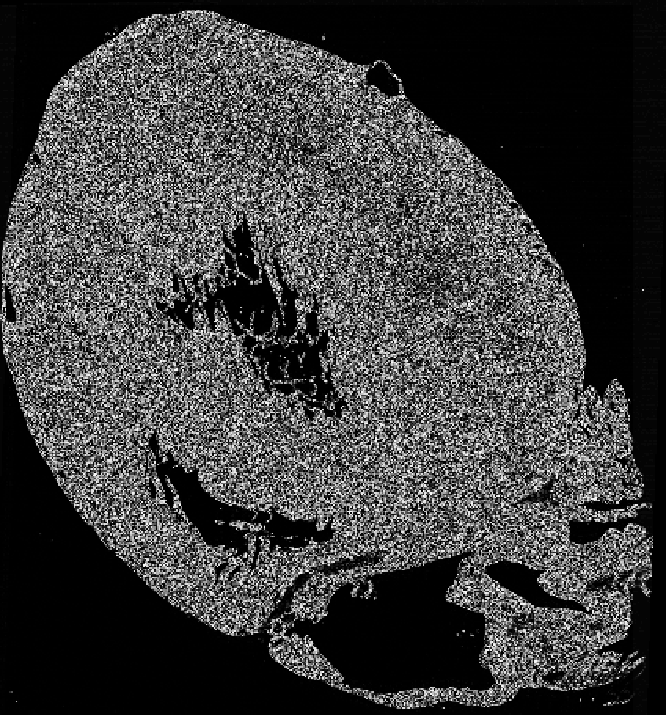
\includegraphics[height=0.365\textheight,type=pdf,ext=.pdf,read=.pdf]{Ch6/Figs/dummies/colour_squared_diff}}
    \caption{Slice 200 from the Rat 28 dataset, the image used used for all test geometries. \textbf{(a)} shows the original image, whilst a small random affine transformation has been applied to \textbf{(b)}. \textbf{(c)} and \textbf{(d)} combine the two slices in two ways, in order to highlight their difference. The mean squared pixel intensity difference in \textbf{(d)} is 61.53.}
    \label{fig:original_displacement}
  \end{figure}
  
  % segmentation slice differences
  \begin{figure}[htbp]
    \centering
    \subfigure[][unperturbed image]{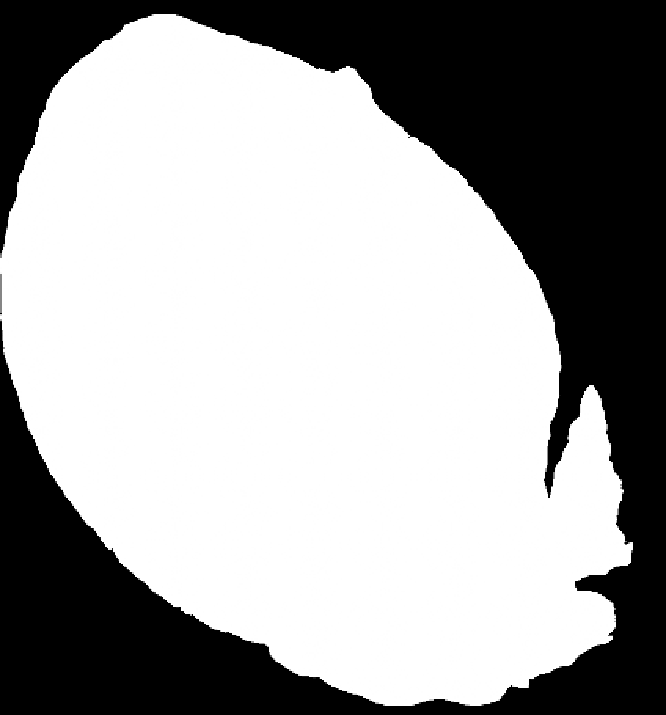
\includegraphics[height=0.365\textheight,type=pdf,ext=.pdf,read=.pdf]{Ch6/Figs/dummies/segmentation_perfect_slice}} \quad
    \subfigure[][image with transformational noise]{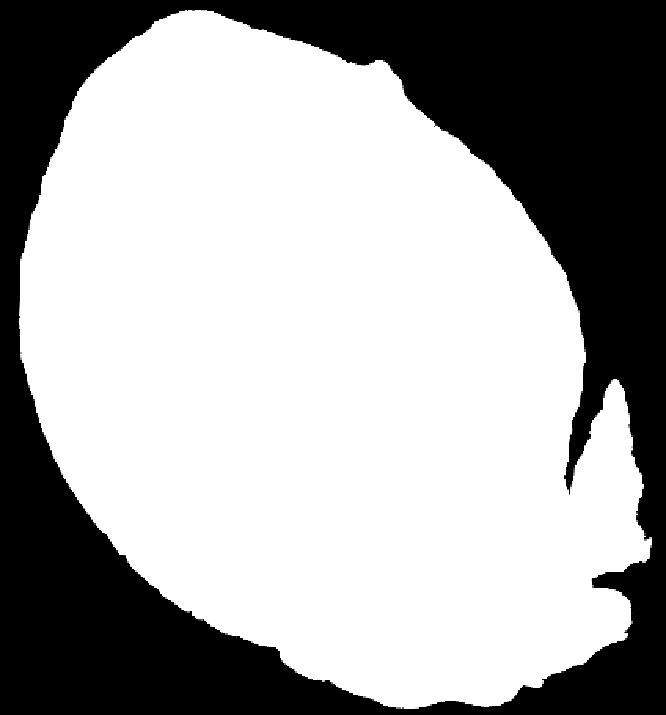
\includegraphics[height=0.365\textheight,type=pdf,ext=.pdf,read=.pdf]{Ch6/Figs/dummies/segmentation_noisy_slice}} \\
    \subfigure[][Red-blue channels of intensities]{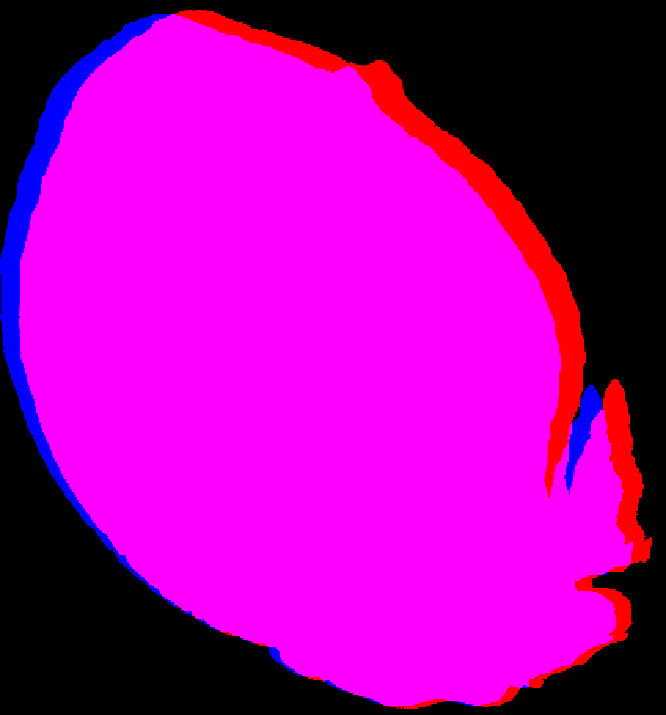
\includegraphics[height=0.365\textheight,type=pdf,ext=.pdf,read=.pdf]{Ch6/Figs/dummies/segmentation_red_blue_diff}} \quad
    \subfigure[][squared differences in intensities]{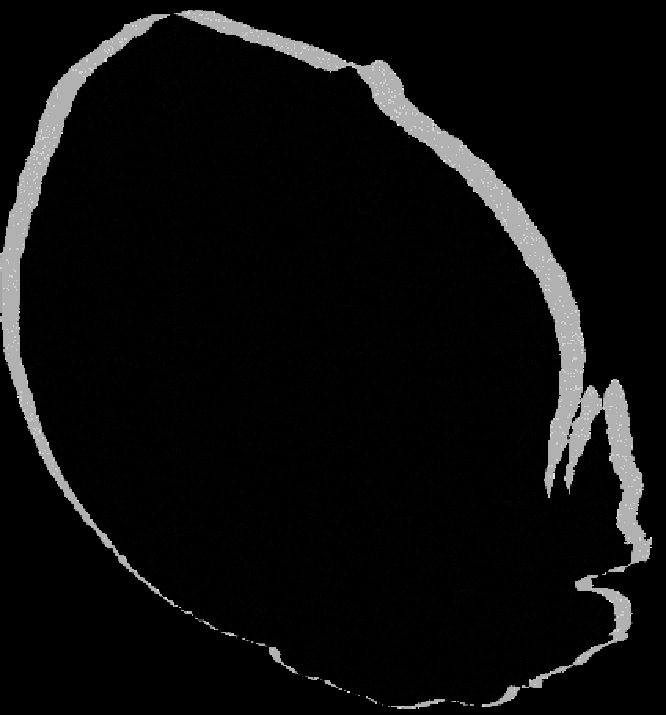
\includegraphics[height=0.365\textheight,type=pdf,ext=.pdf,read=.pdf]{Ch6/Figs/dummies/segmentation_squared_diff}}
    \caption{A manual segmentation of the same slice from Figure~\ref{fig:original_displacement}, with the same perturbation applied. The noise in the squared intensity differences in Figure~\ref{fig:original_displacement}~\textbf{(d)} are no longer present. This leads to a much smoother cost function, with much fewer local minima, and thus a more reliable registration. The improvement is reflected in the lower mean squared pixel intensity difference in \textbf{(d)} of 12.93.}
    \label{fig:segmented_displacement}
  \end{figure}
  
  The process of registration between slices, of obtaining the values $\mathbf{\Delta T}_{i,i+1}^n$, is orthogonal to and separate from the calculation of the diffusion transforms $\mathbf{\Delta T}_i^{n,n+1}$ and subsequent adjustment of each slice transform $\mathbf{T}_i^{n+1}$. The first attempt to test the algorithm used the original heart slice image shown in Figure~\ref{fig:original_displacement}. Although the algorithm was reliably stable in smoothing the small amplitudes of noise it was designed to correct for, it was found that much larger perturbations could be damped by the algorithm, limited only by the success of the individual registrations. All registrations were therefore performed using the manual segmentations shown in Figure~\ref{fig:segmented_displacement}, with which much larger displacements could be corrected. As will be seen, cross-sections were then reconstructed from the original images, to show the effects of correction on the fine detail of the tissue, whilst clean volume isosurfaces were constructed from the segmentation.
  
  % straight
  \begin{figure}[htbp]
    \centering
    % filename format: cross_section_200_alpha0.4_ITERATION_DIMENSION_SLICE
    \subfigure[][with noise (0 iterations)]{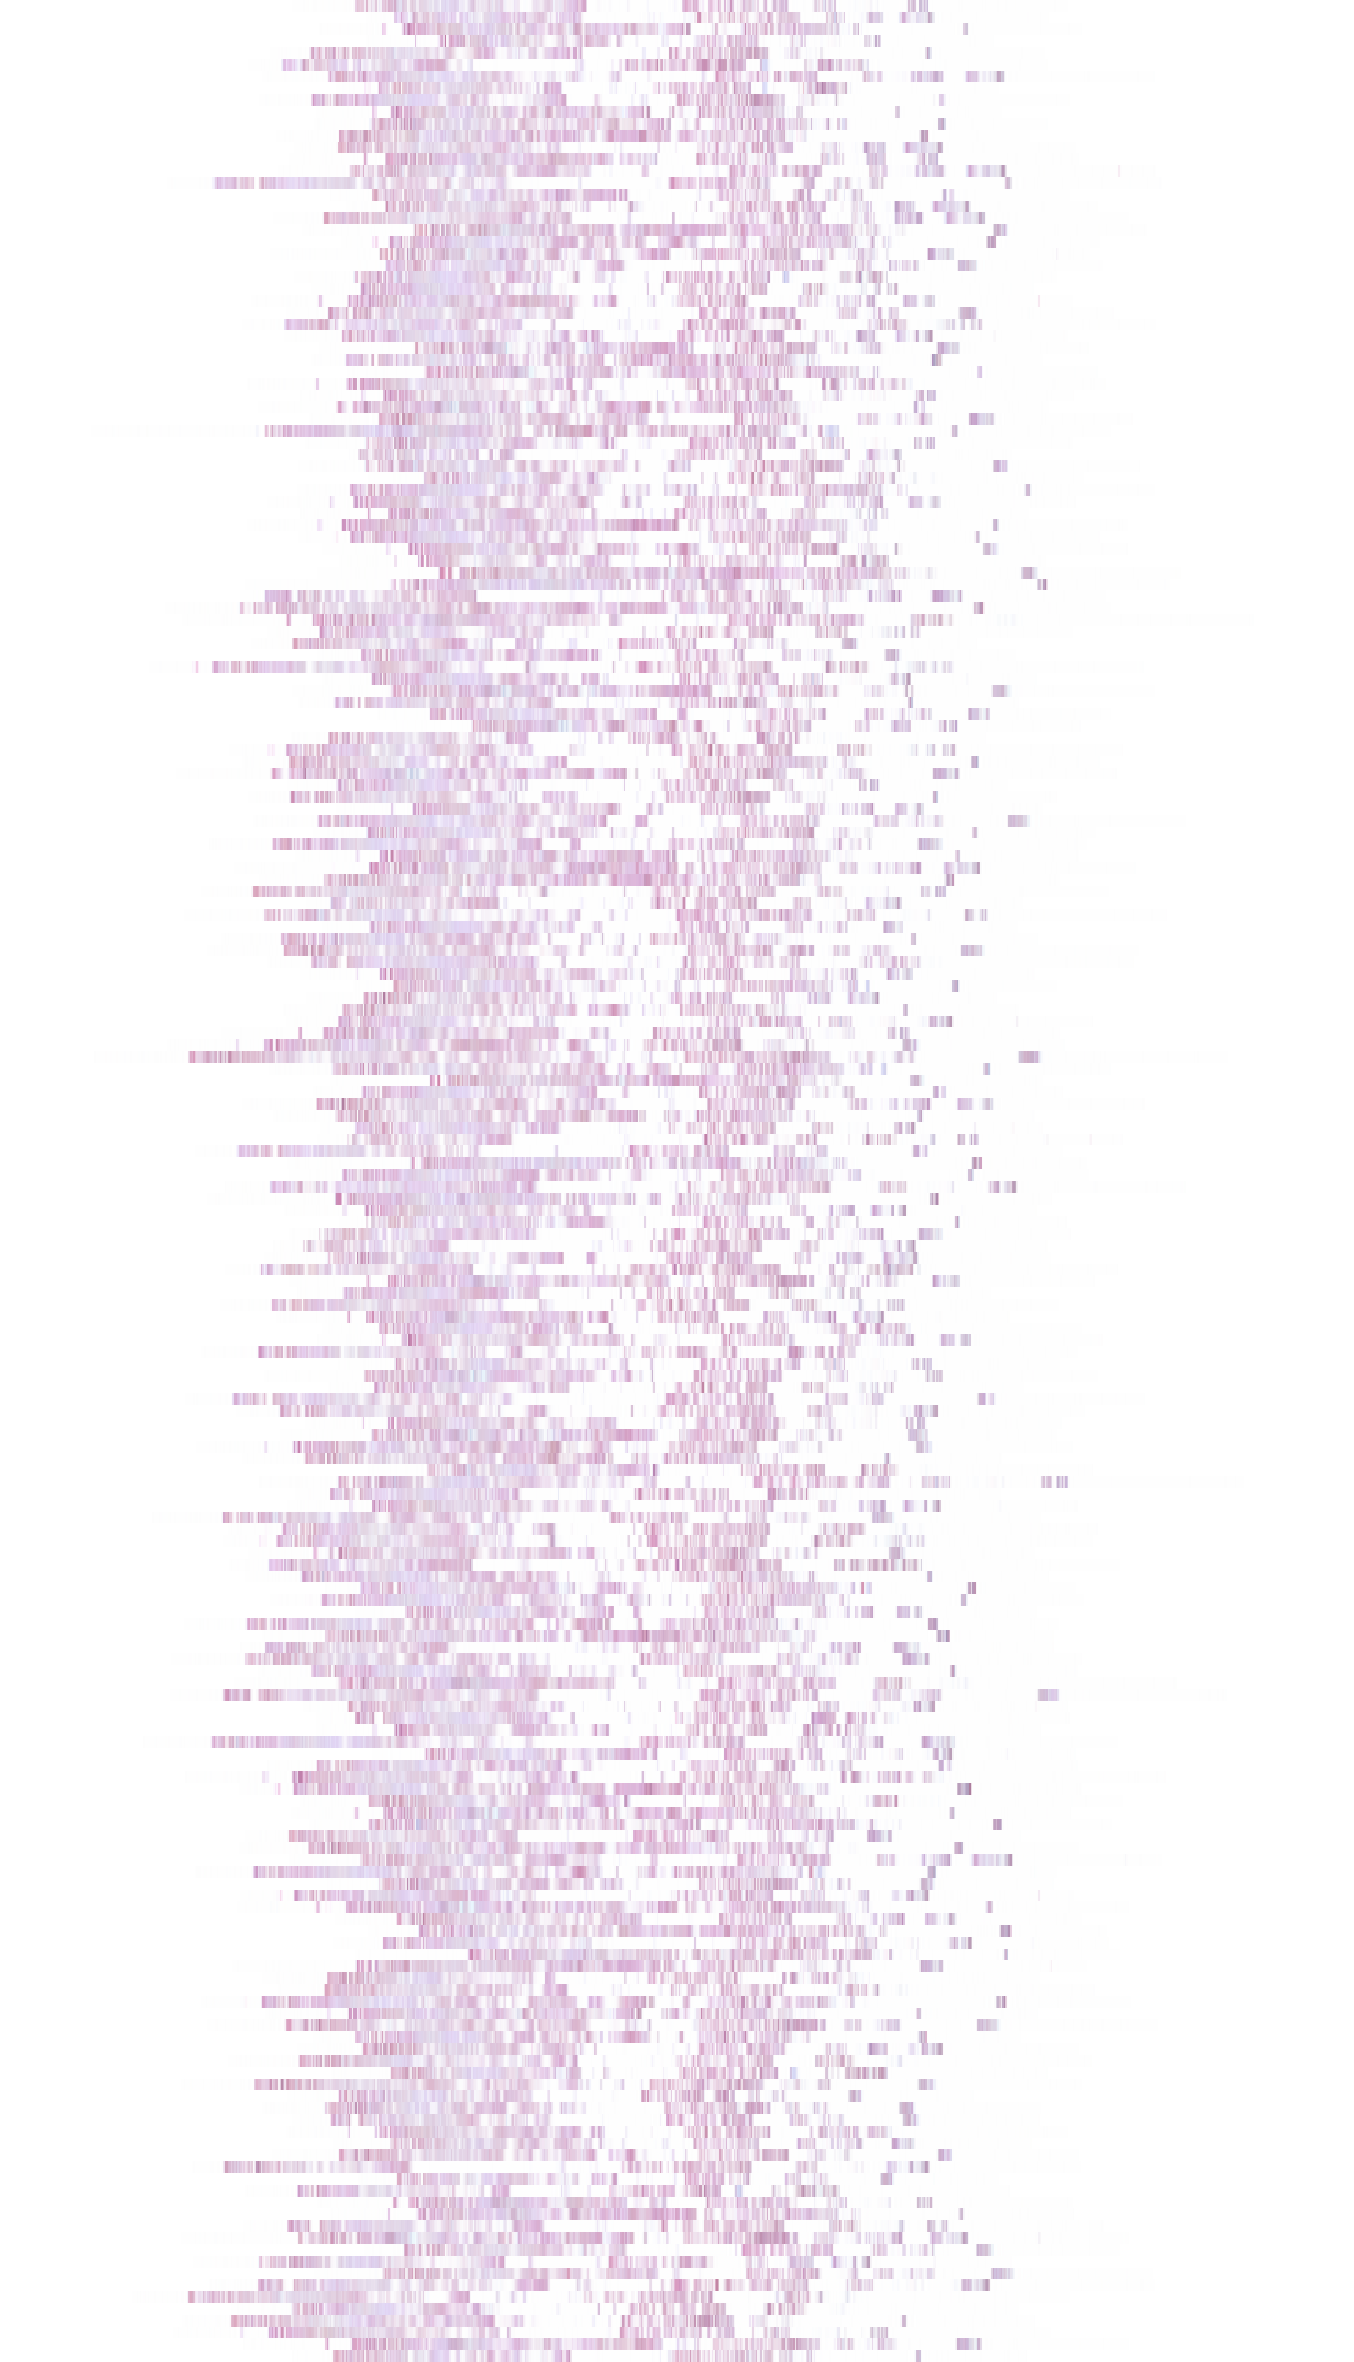
\includegraphics[height=0.4\textheight,type=pdf,ext=.pdf,read=.pdf]{Ch6/Figs/dummies/cross_section_200_alpha0.4_0_0_352}\label{fig:subfig1}}
    \subfigure[][1 iteration]{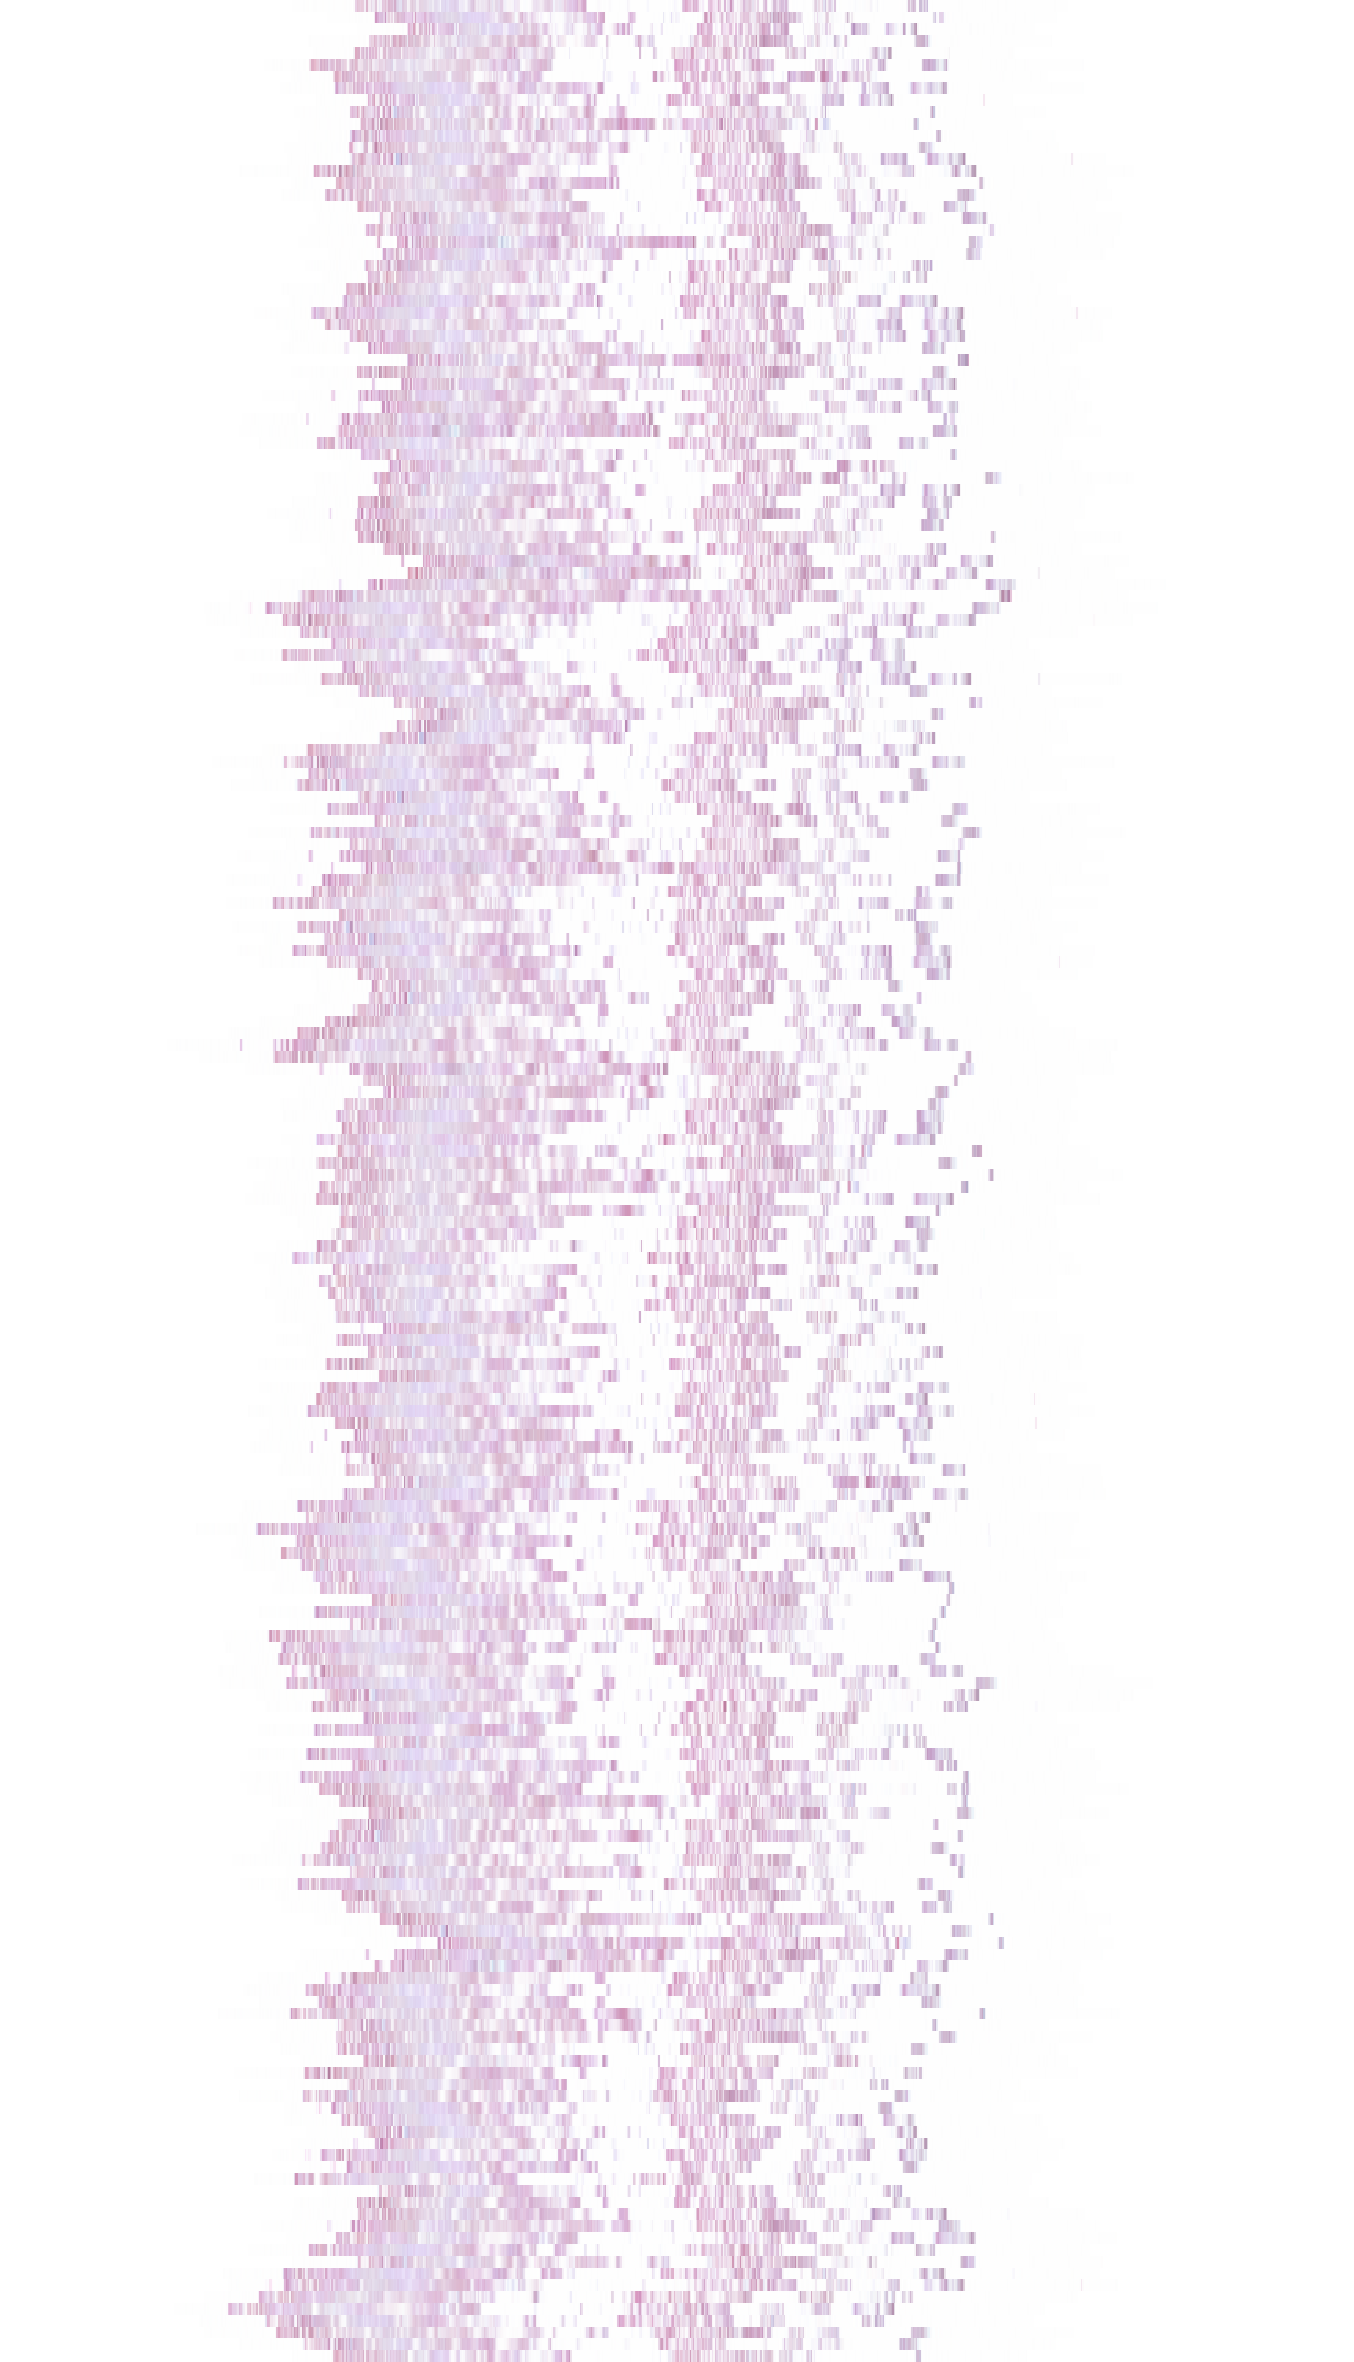
\includegraphics[height=0.4\textheight,type=pdf,ext=.pdf,read=.pdf]{Ch6/Figs/dummies/cross_section_200_alpha0.4_1_0_352}\label{fig:subfig2}}
    \subfigure[][3 iterations]{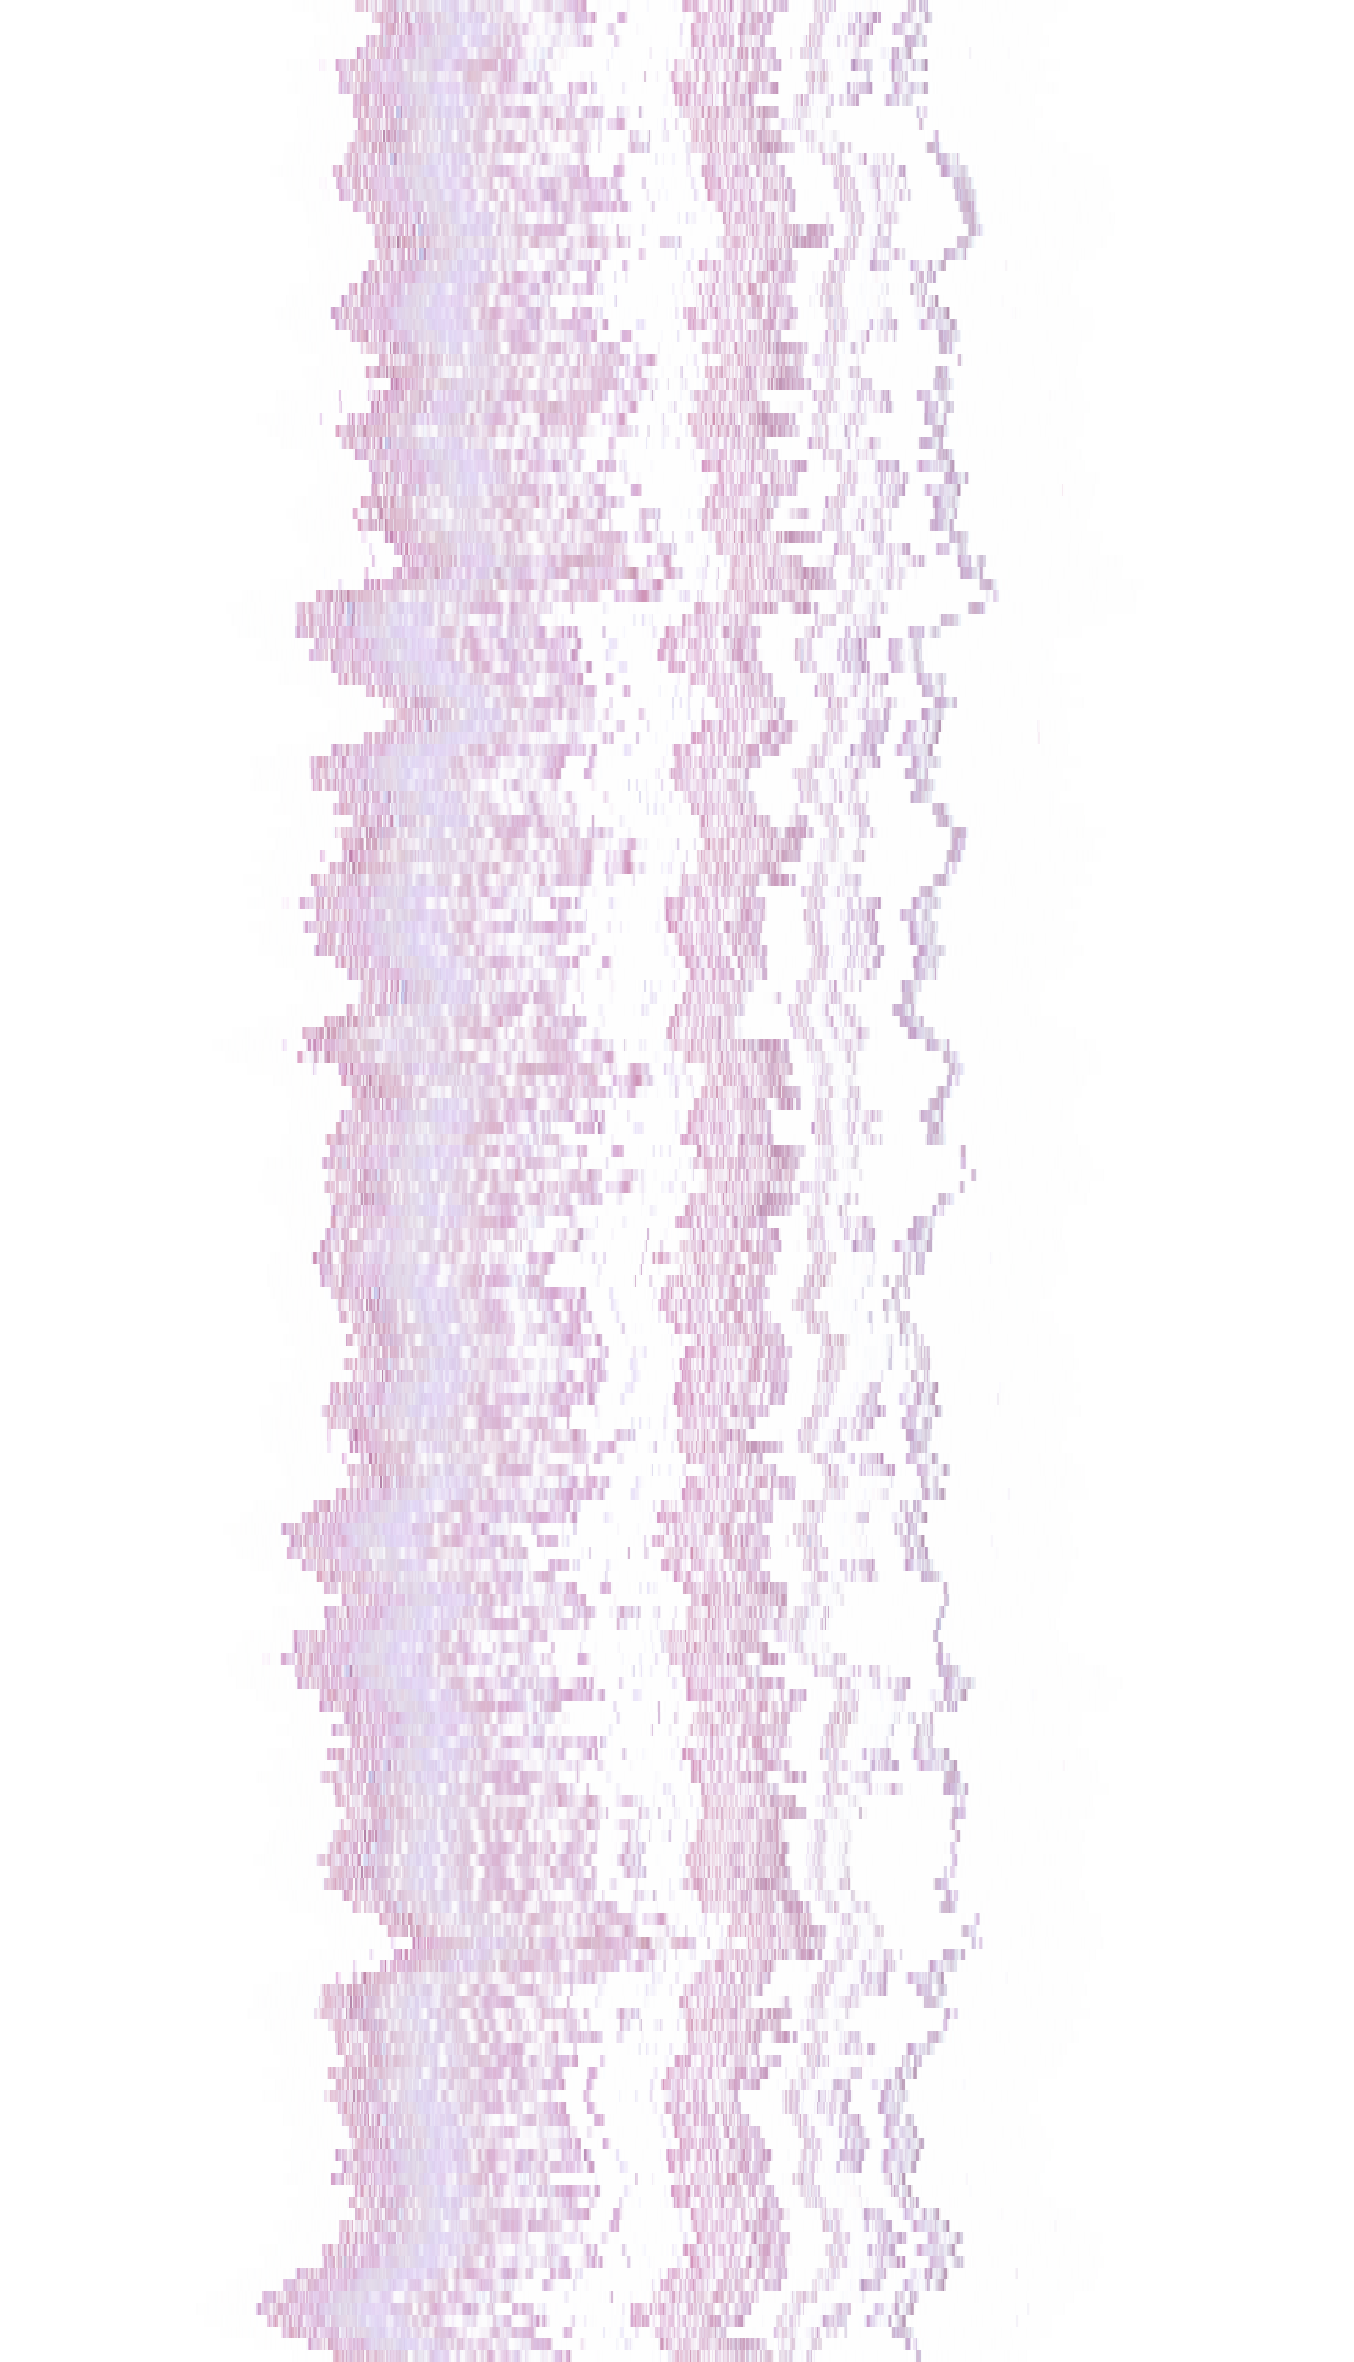
\includegraphics[height=0.4\textheight,type=pdf,ext=.pdf,read=.pdf]{Ch6/Figs/dummies/cross_section_200_alpha0.4_3_0_352}\label{fig:subfig3}}
    \subfigure[][8 iterations]{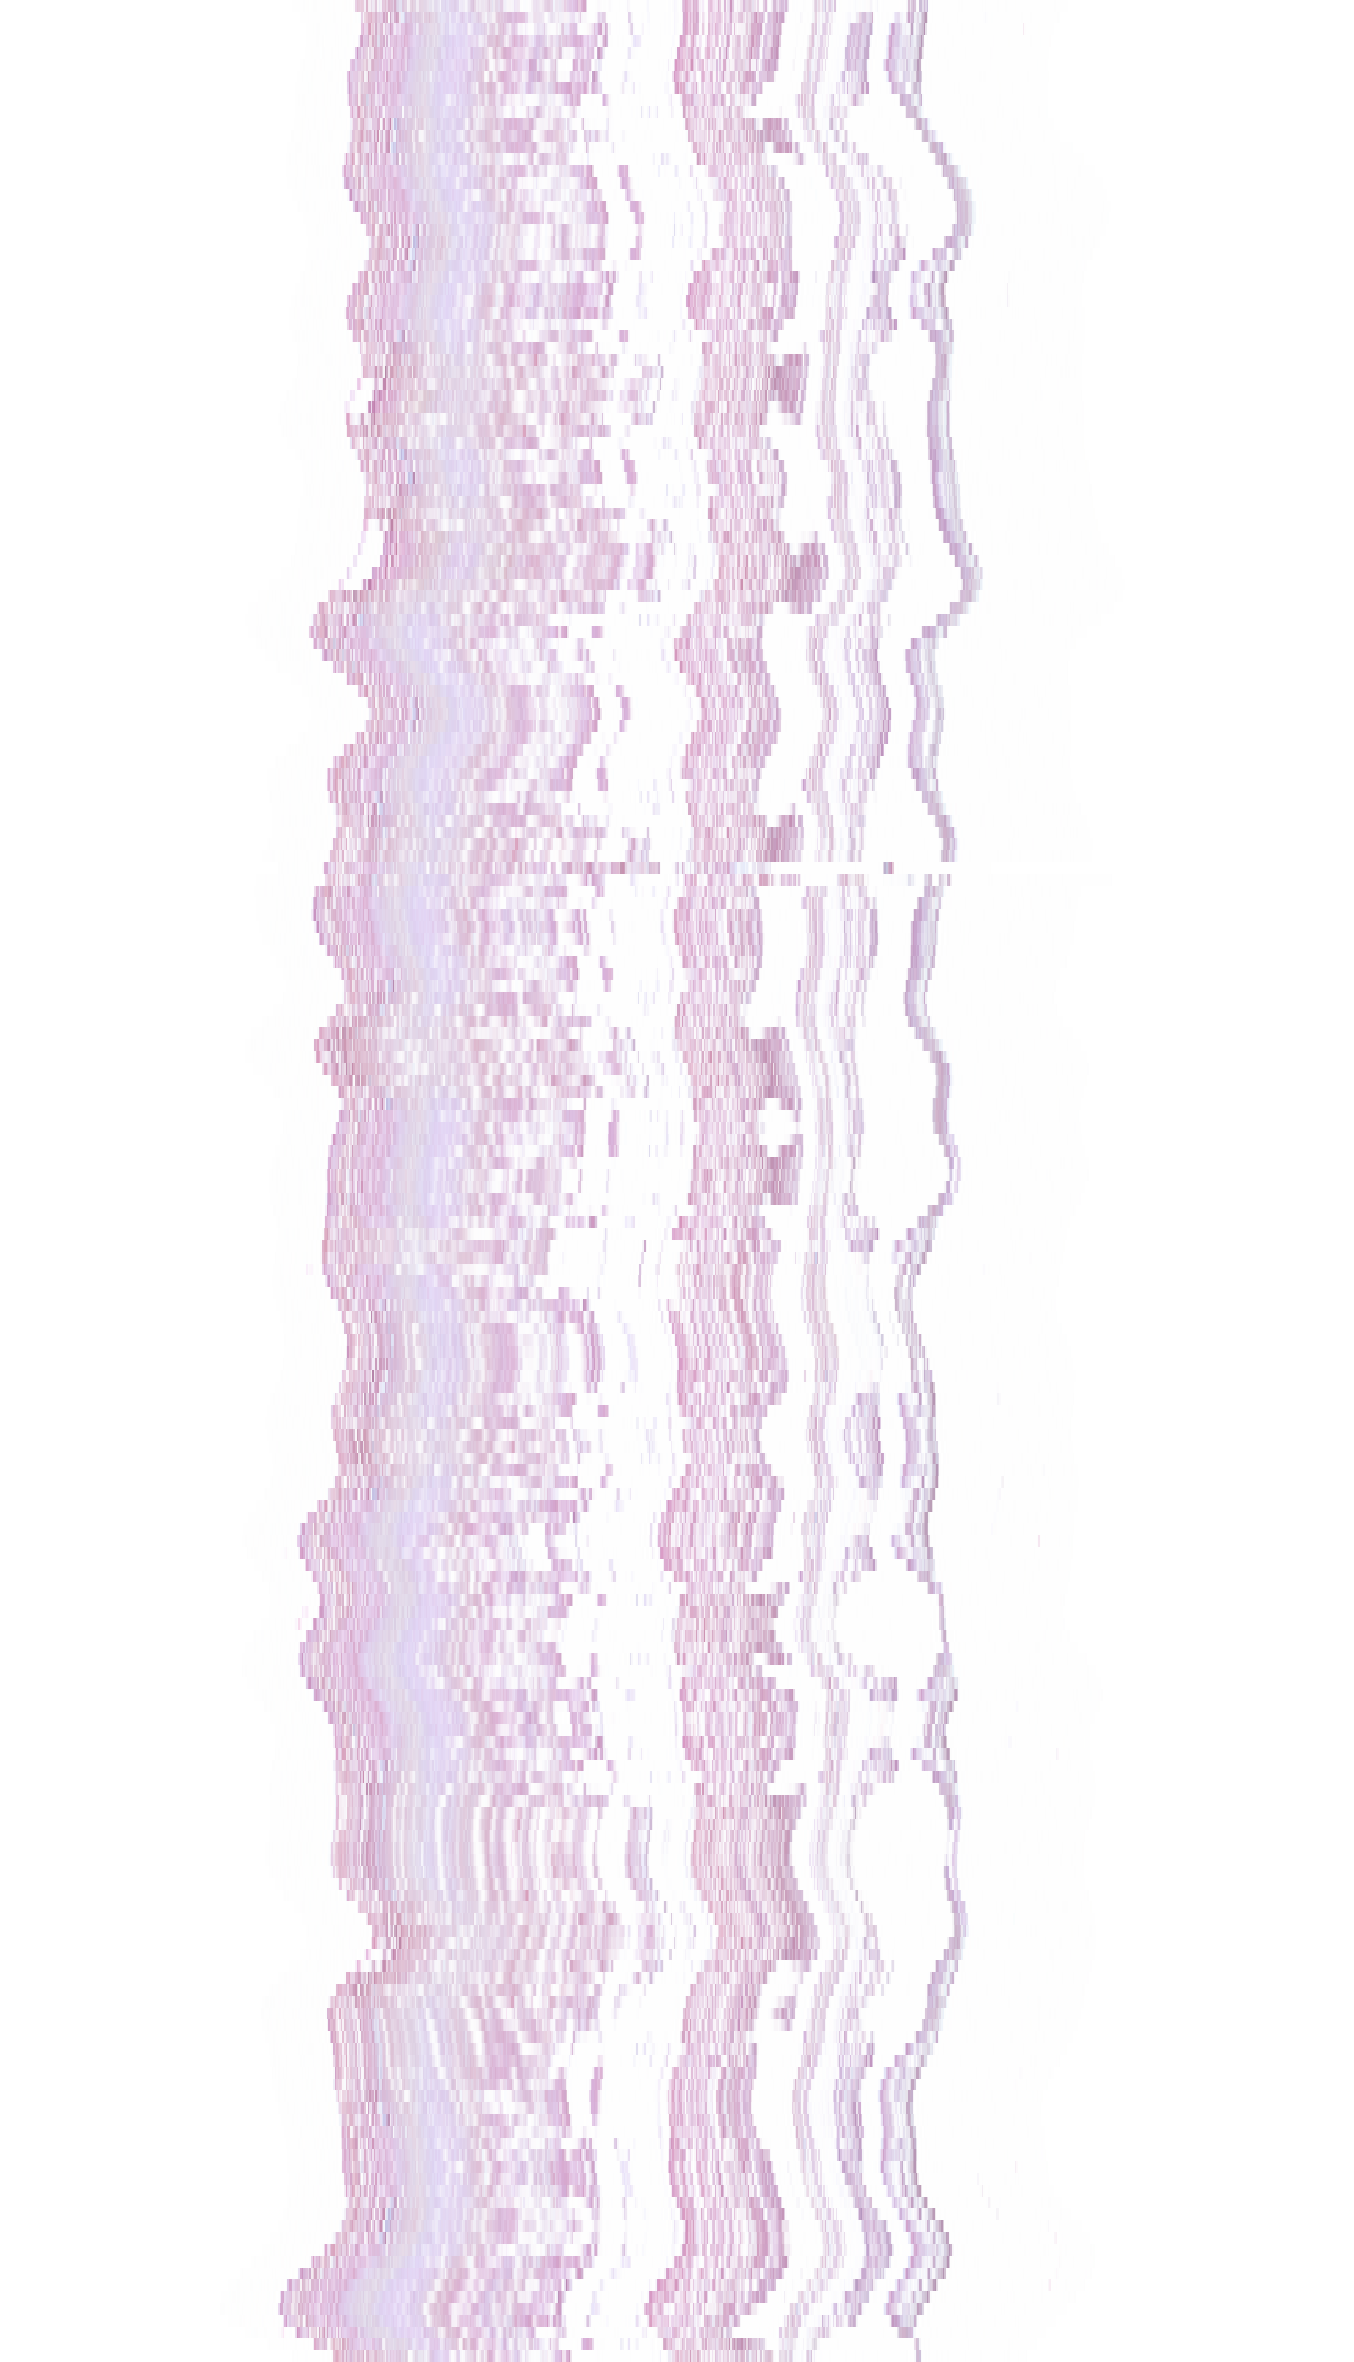
\includegraphics[height=0.4\textheight,type=pdf,ext=.pdf,read=.pdf]{Ch6/Figs/dummies/cross_section_200_alpha0.4_8_0_352}\label{fig:subfig4}}
    \subfigure[][20 iterations]{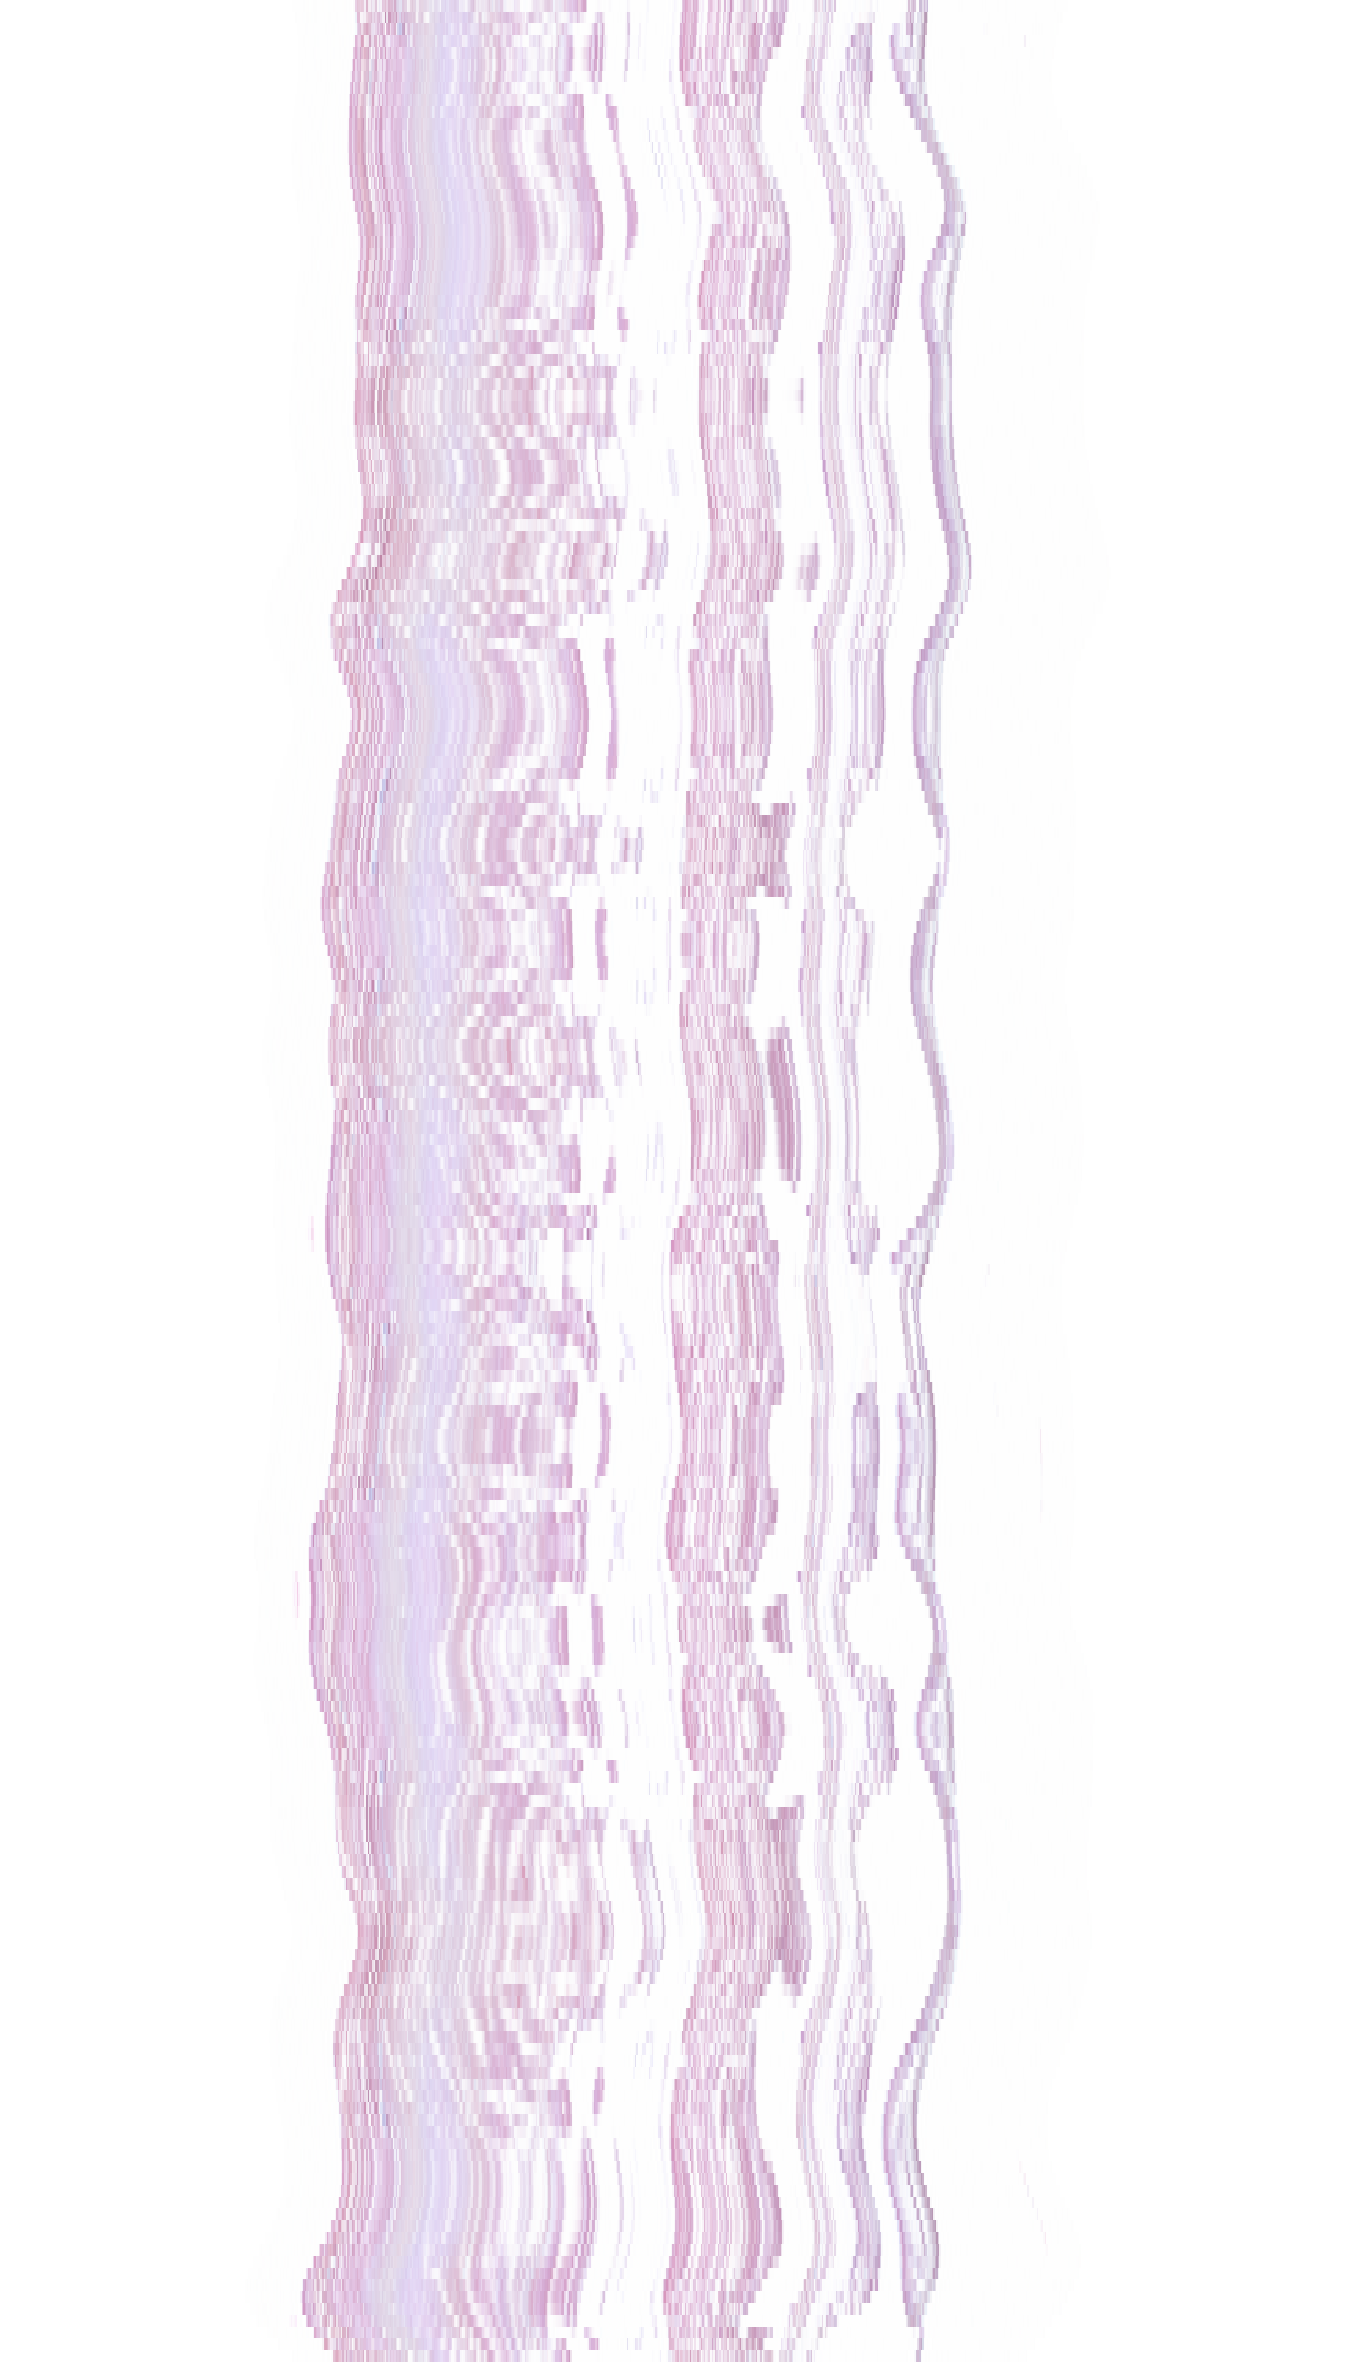
\includegraphics[height=0.4\textheight,type=pdf,ext=.pdf,read=.pdf]{Ch6/Figs/dummies/cross_section_200_alpha0.4_20_0_352}\label{fig:subfig4}}
    % filename format: cross_section_perfect_200_alpha0.4_DIMENSION_SLICE
    \subfigure[][without noise]{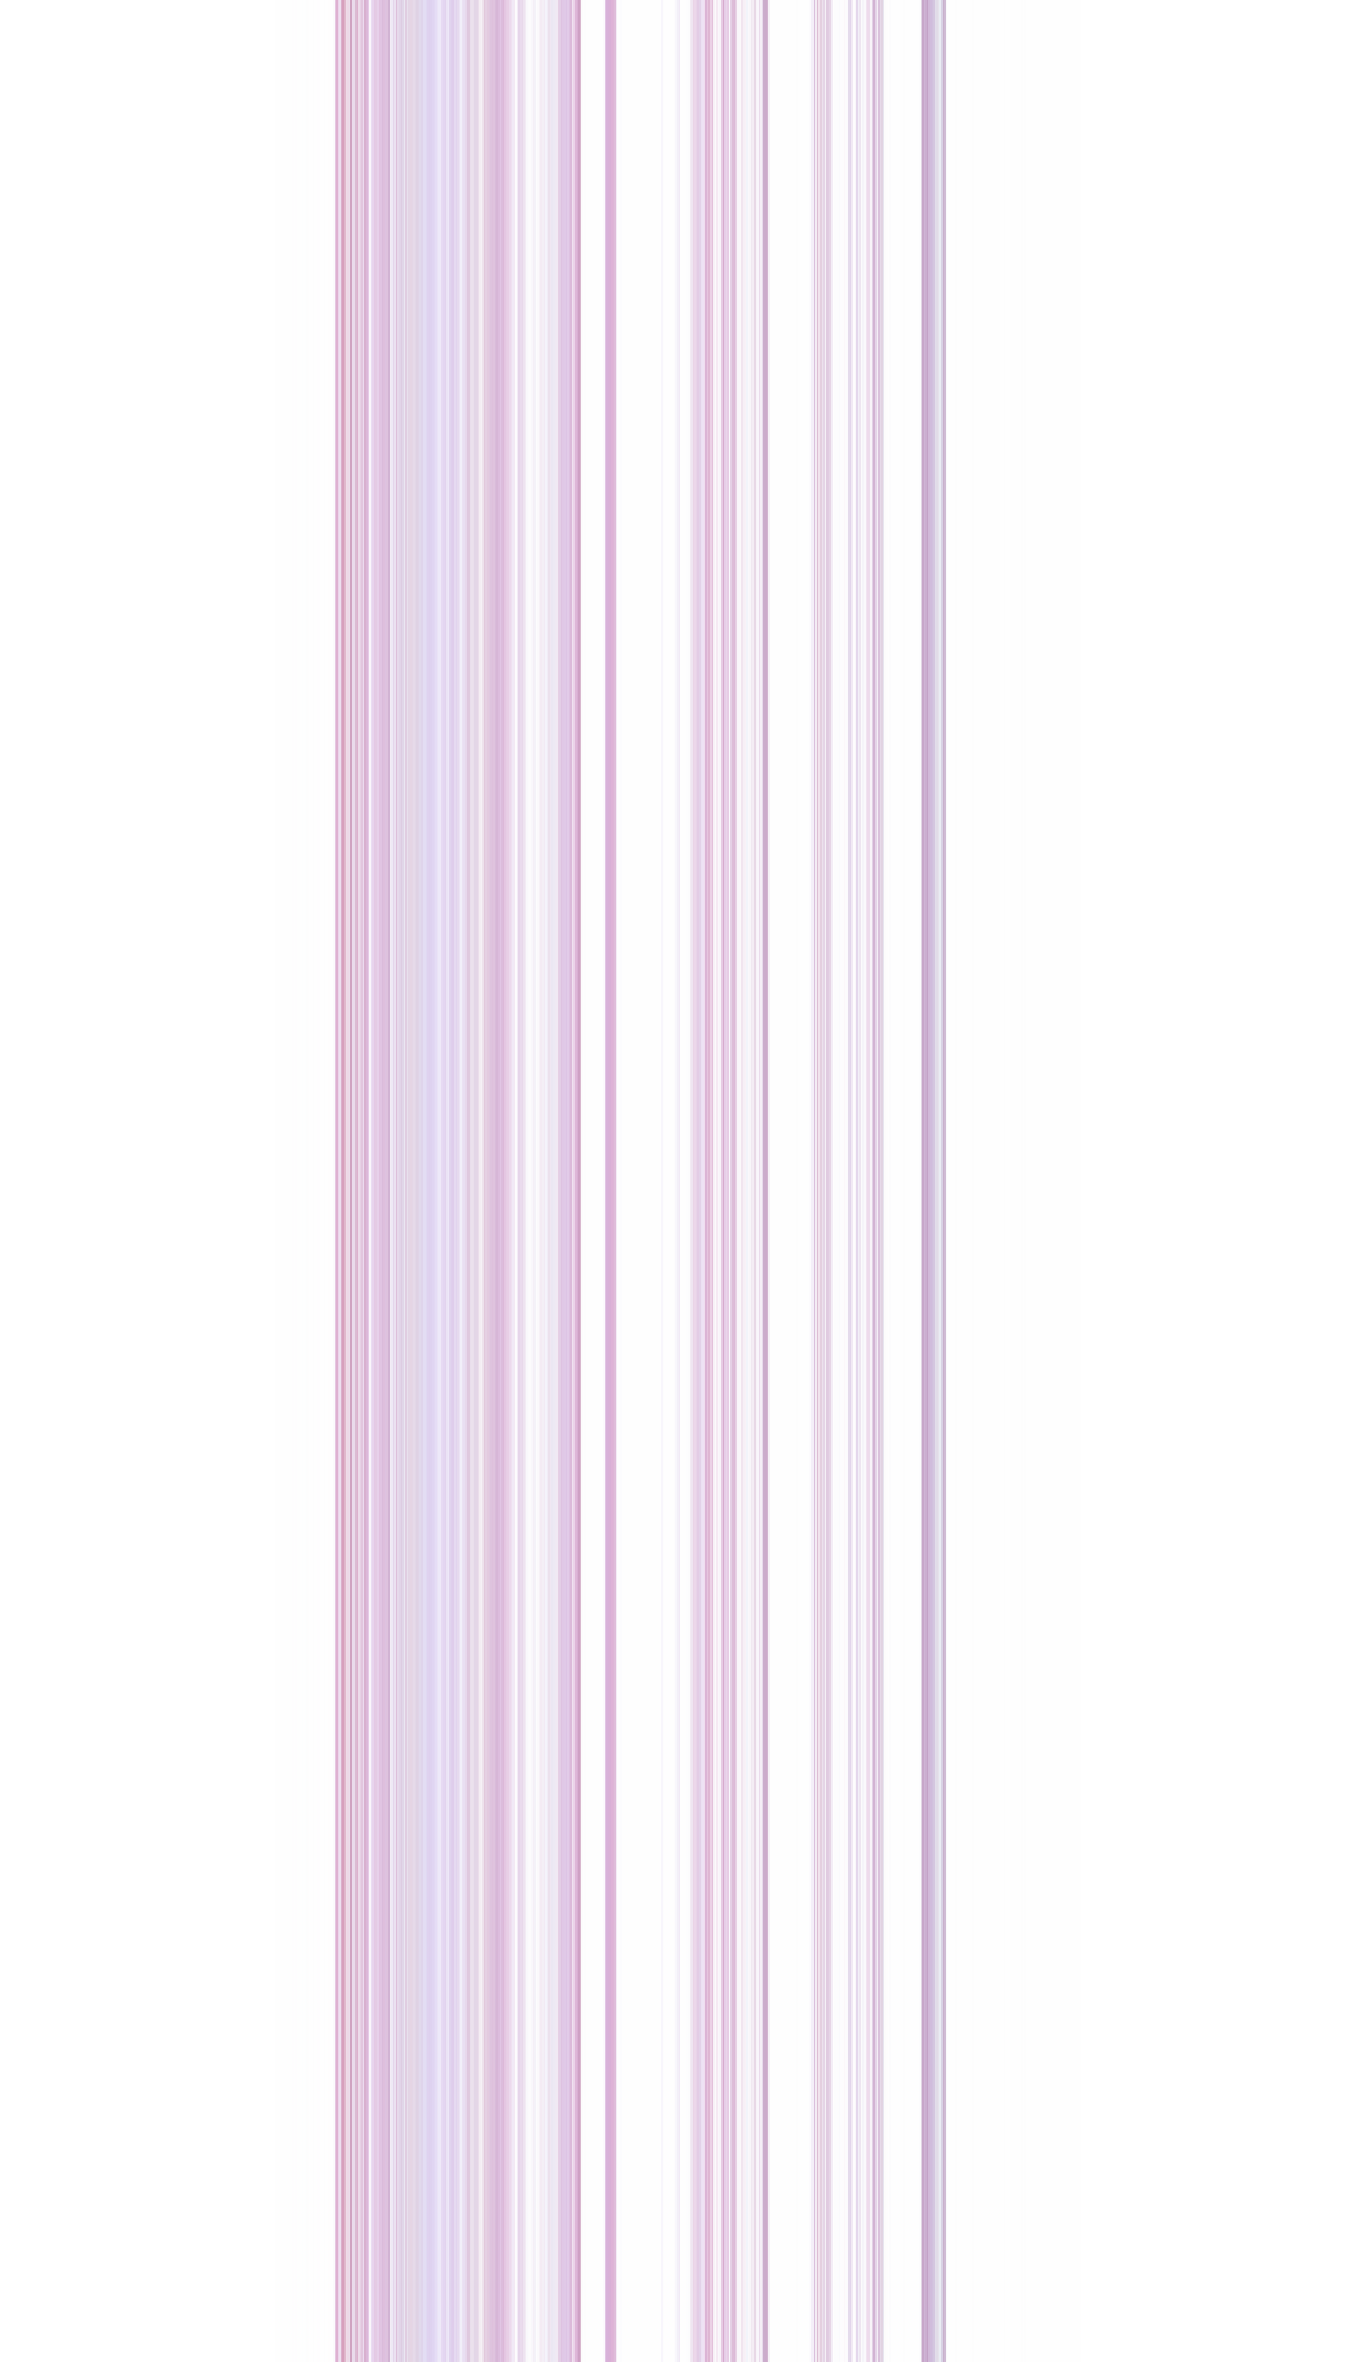
\includegraphics[height=0.4\textheight,type=pdf,ext=.pdf,read=.pdf]{Ch6/Figs/dummies/cross_section_perfect_200_alpha0.4_0_352}}
    \caption{Cross-sections of the straight volume, perpendicular to the x-axis.}
    \label{fig:cross_section_0}
  \end{figure}
  
  \begin{figure}[htbp]
    \centering
    \subfigure[][0 iterations]{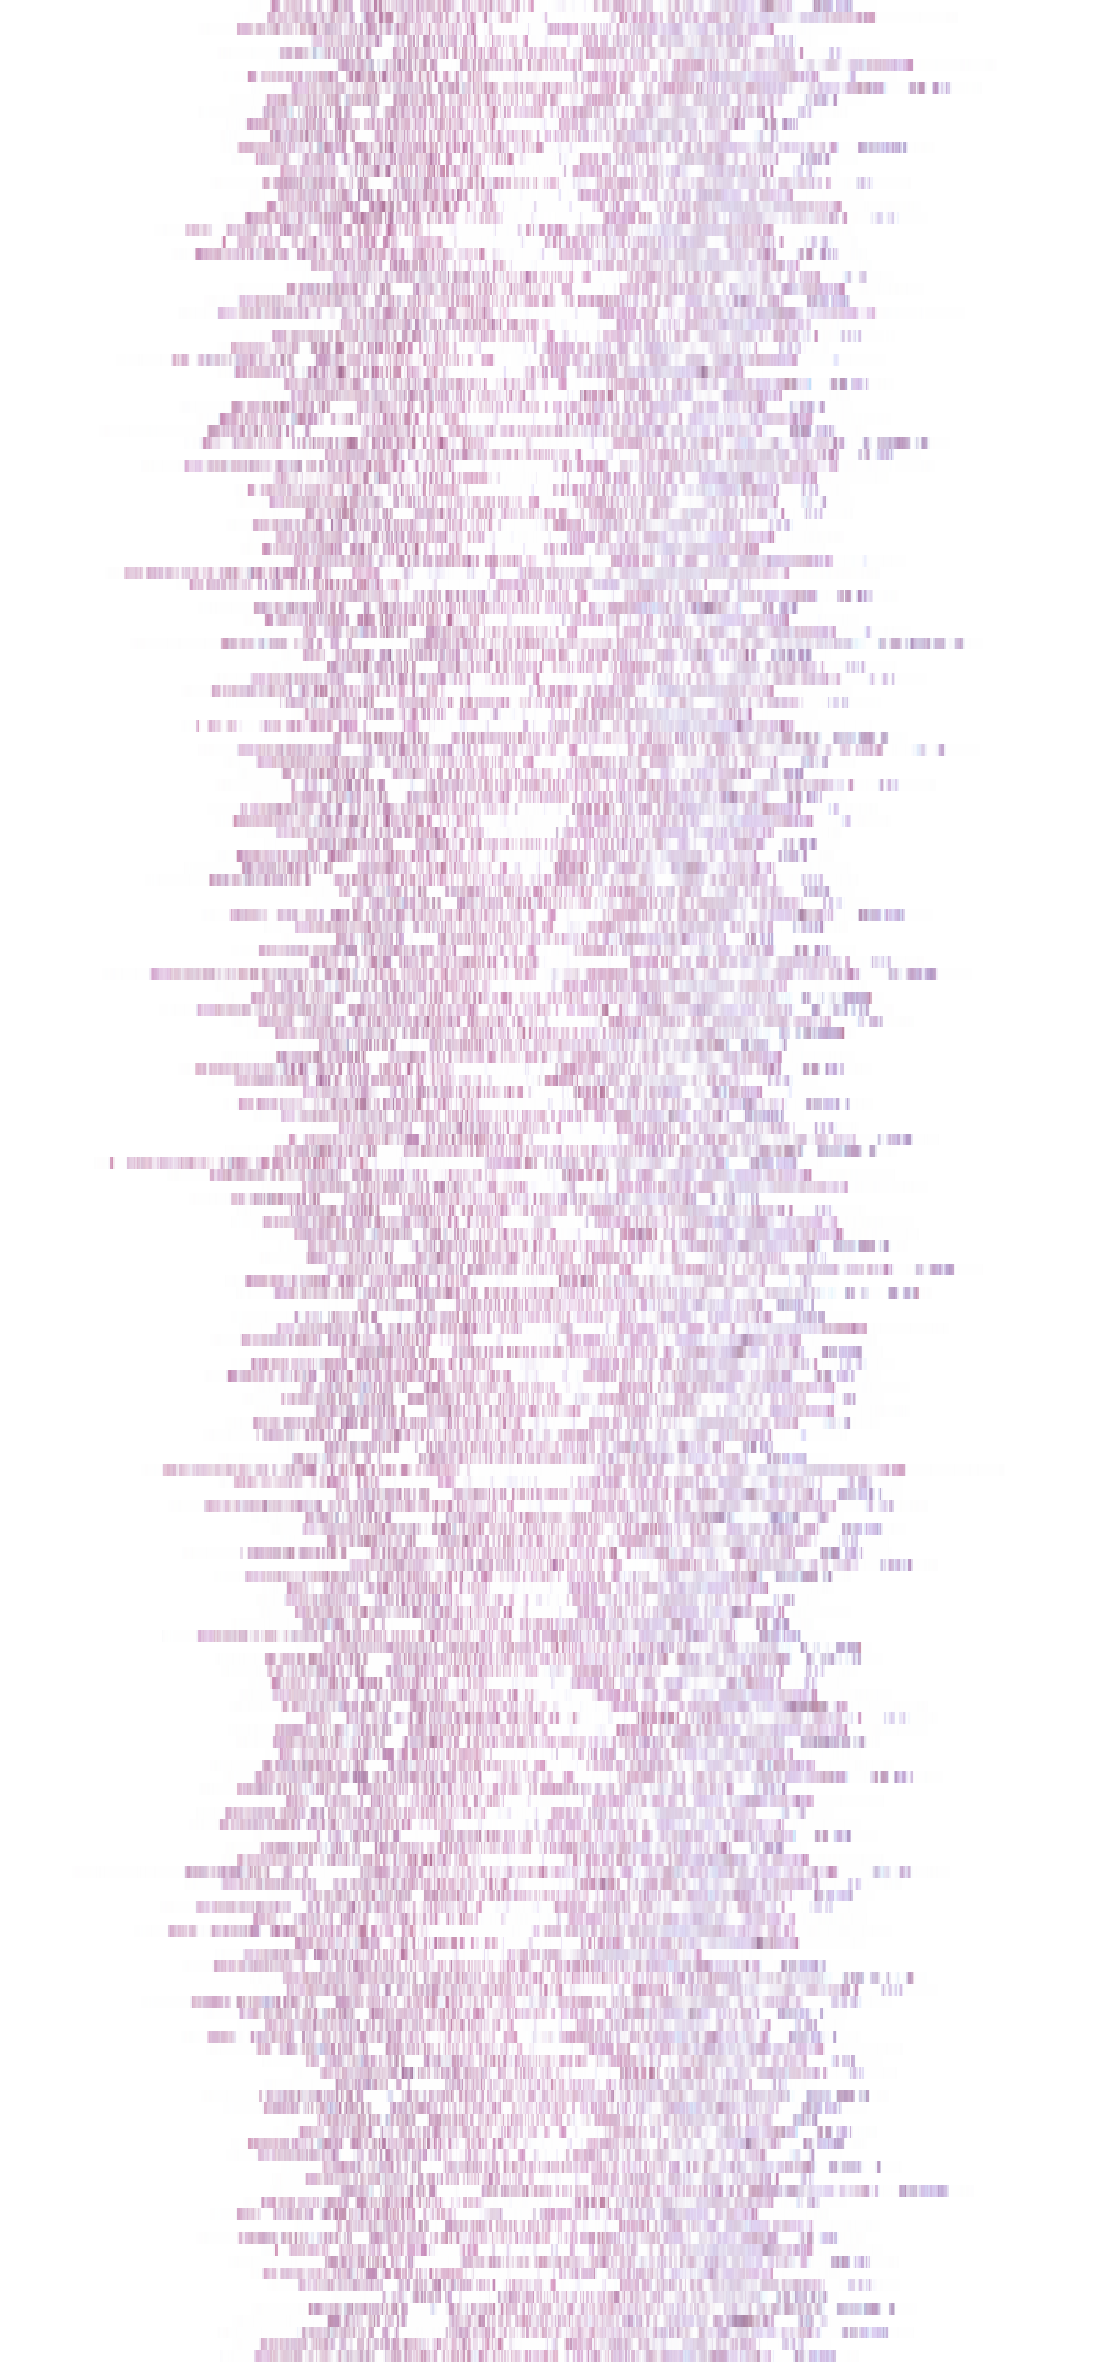
\includegraphics[height=0.4\textheight,type=pdf,ext=.pdf,read=.pdf]{Ch6/Figs/dummies/cross_section_200_alpha0.4_0_1_431}}
    \subfigure[][1 iteration]{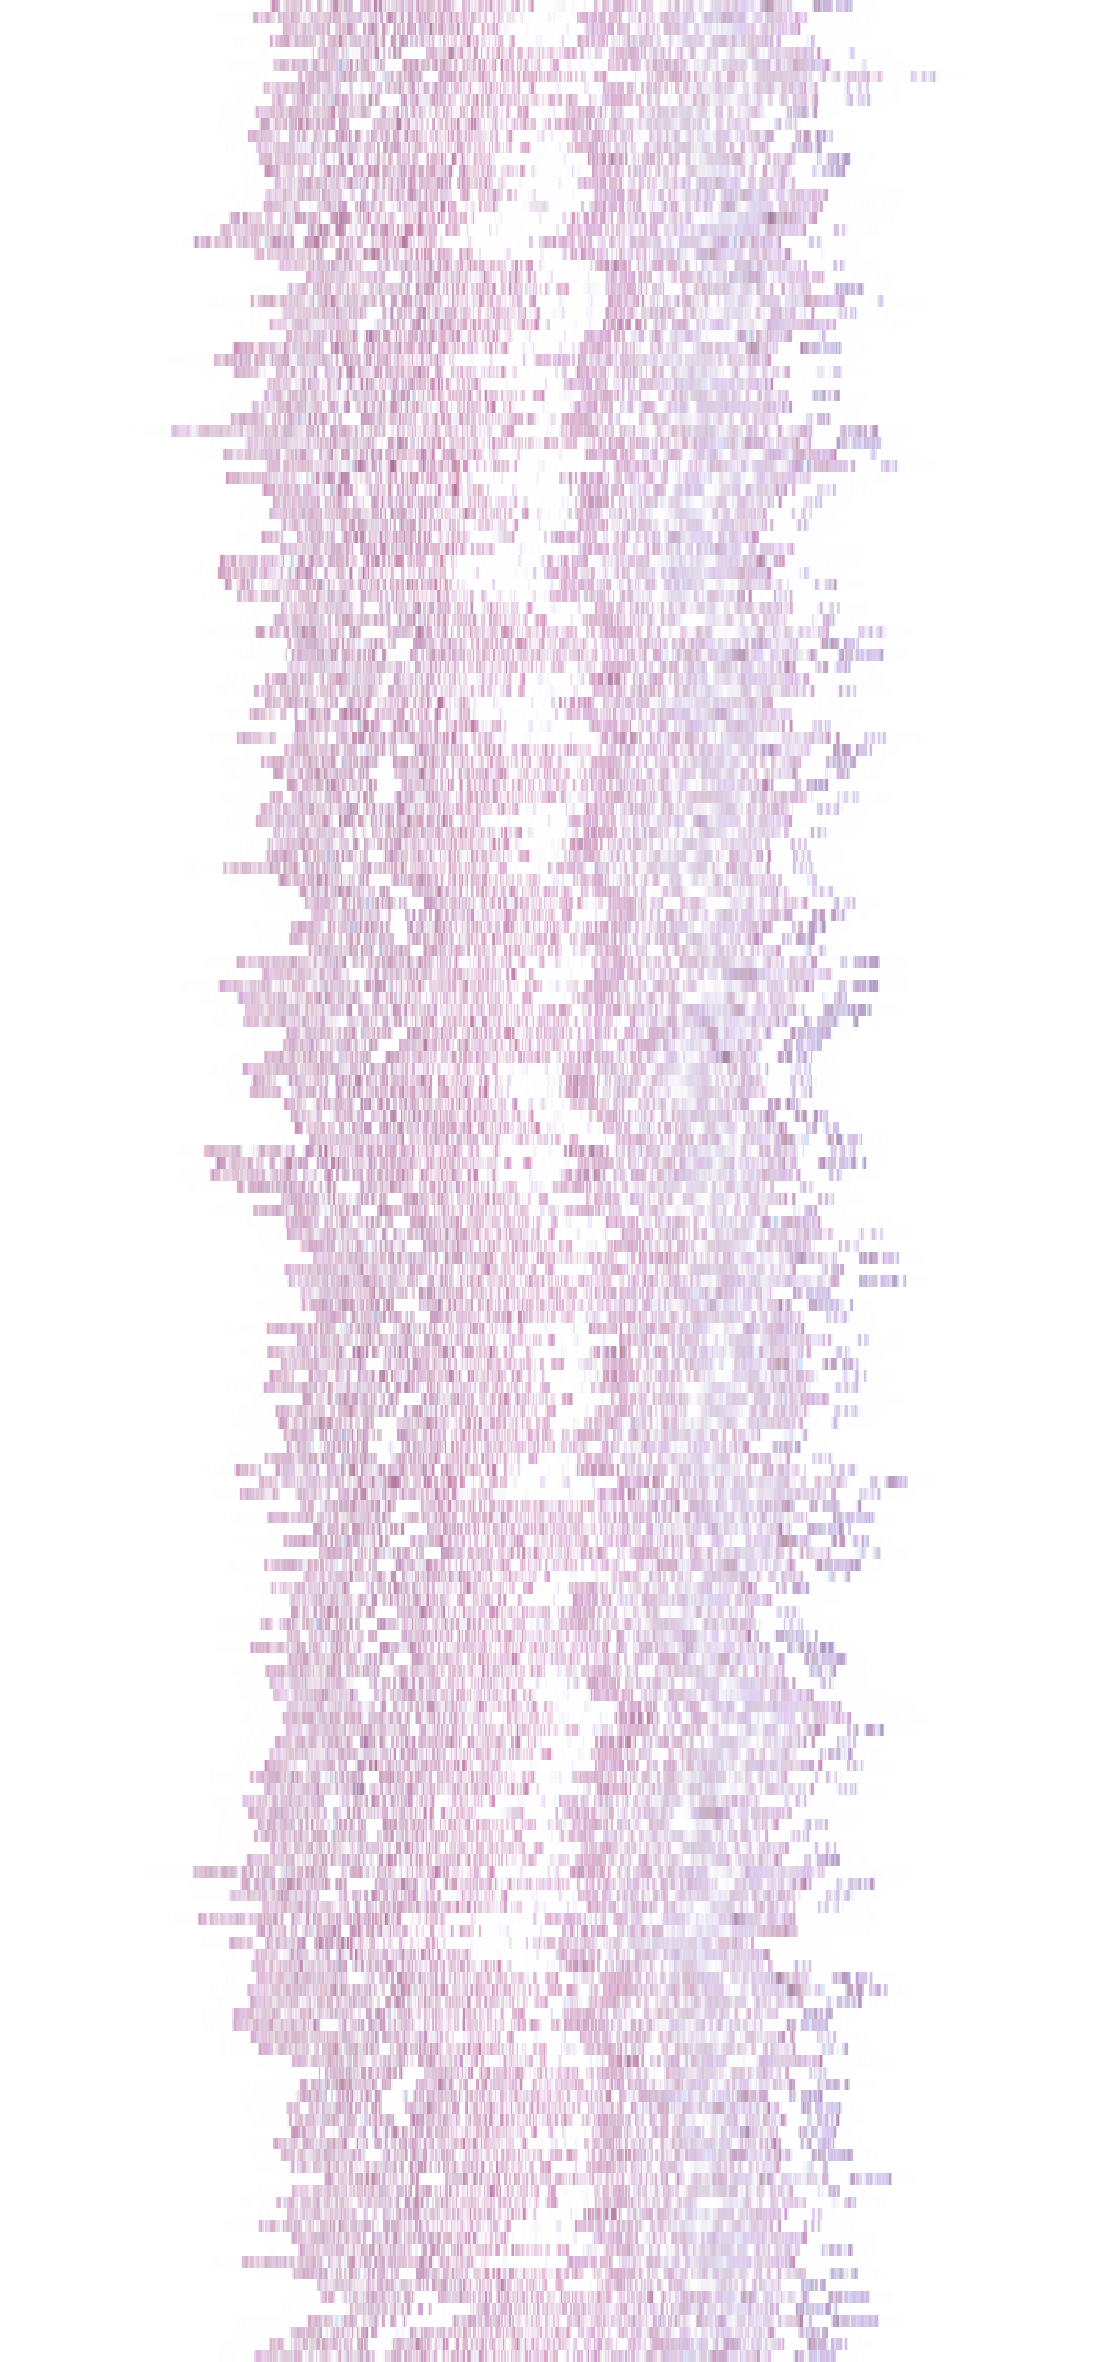
\includegraphics[height=0.4\textheight,type=pdf,ext=.pdf,read=.pdf]{Ch6/Figs/dummies/cross_section_200_alpha0.4_1_1_431}}
    \subfigure[][3 iterations]{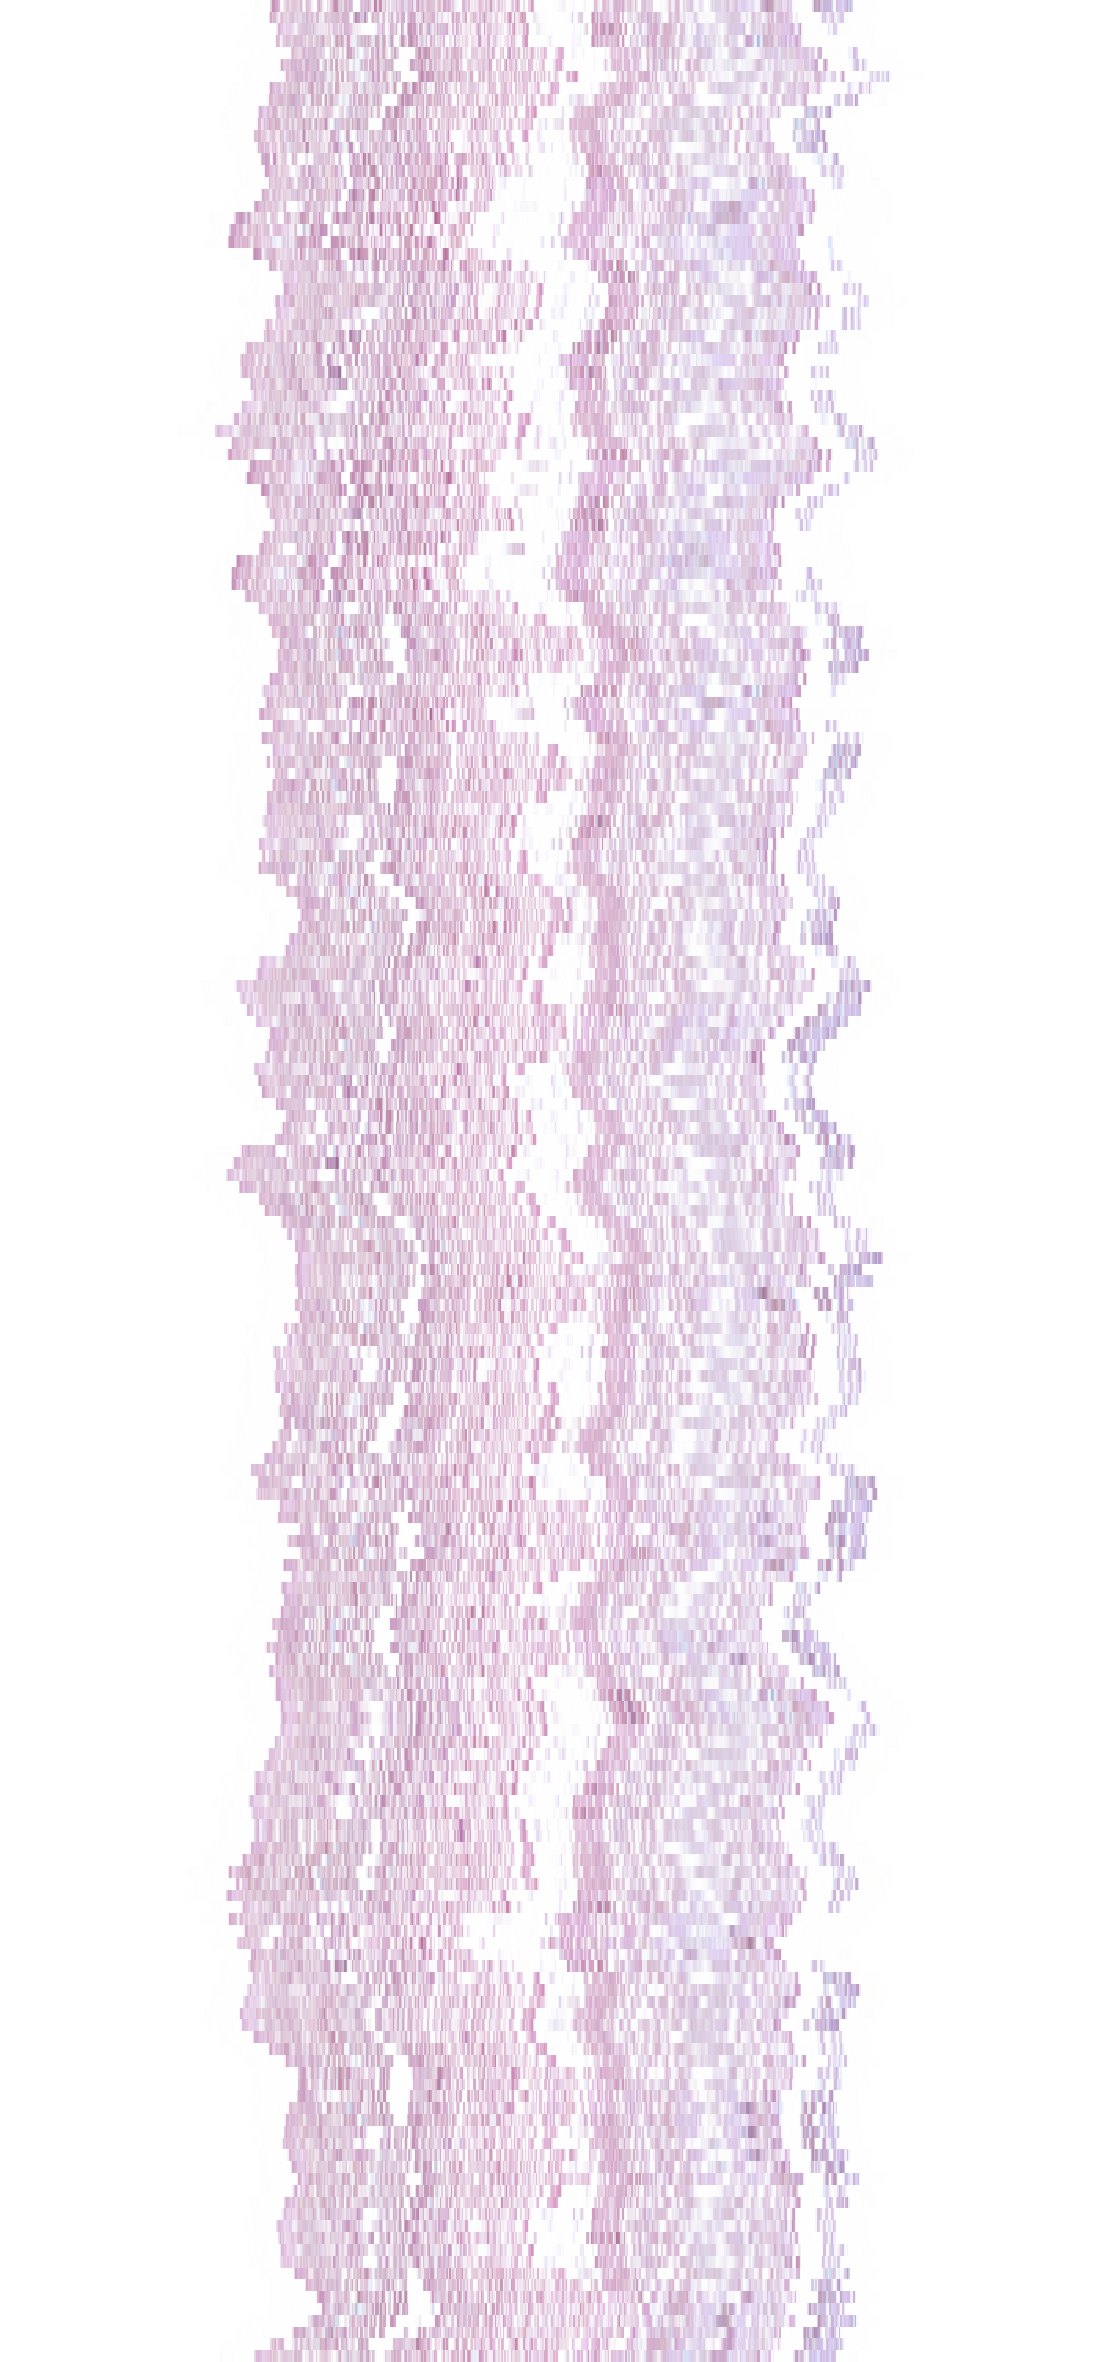
\includegraphics[height=0.4\textheight,type=pdf,ext=.pdf,read=.pdf]{Ch6/Figs/dummies/cross_section_200_alpha0.4_3_1_431}}
    \subfigure[][8 iterations]{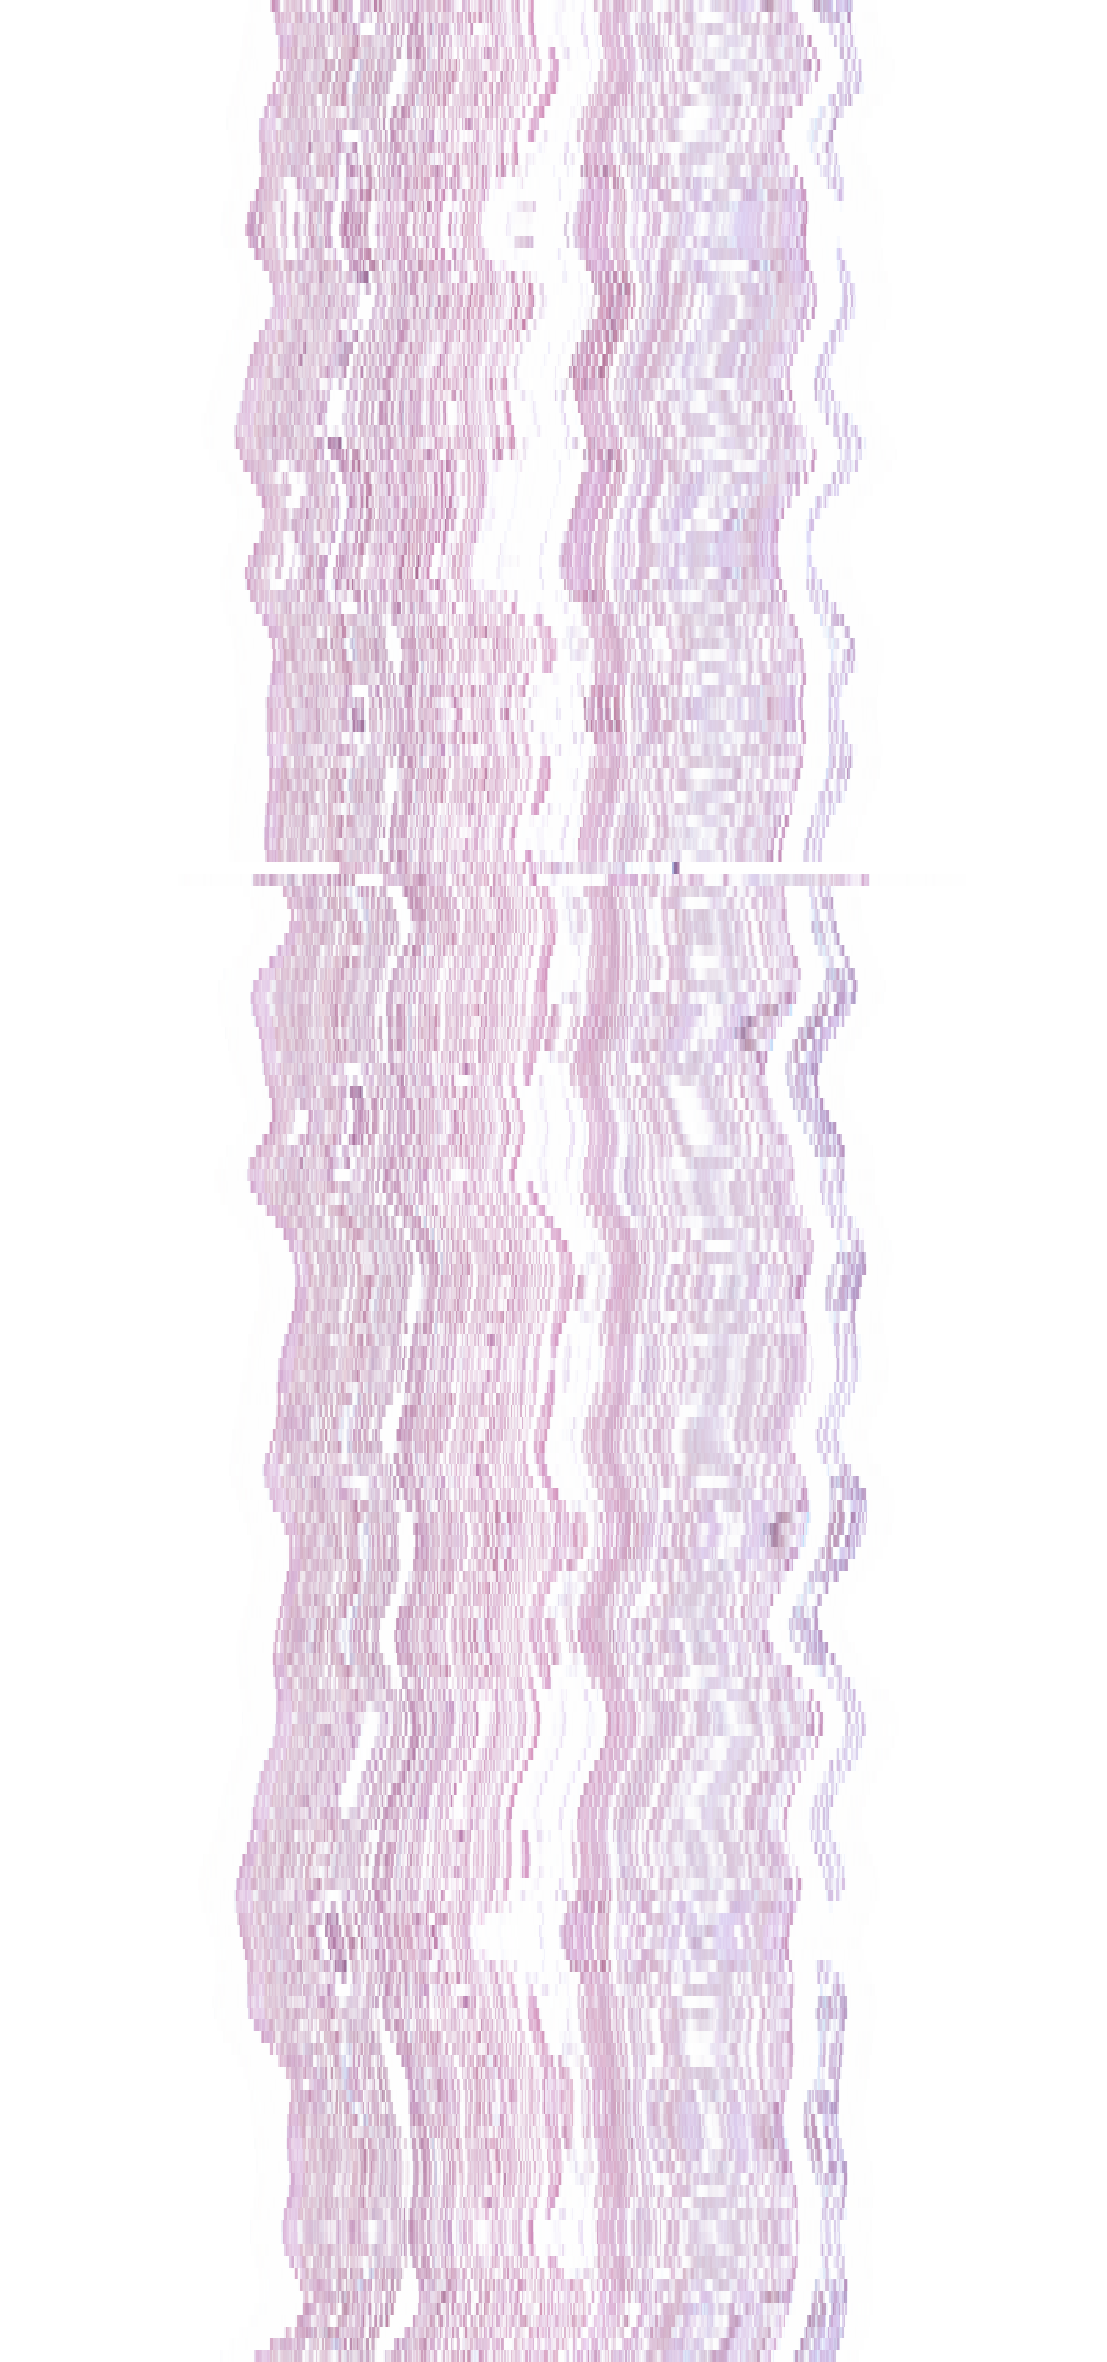
\includegraphics[height=0.4\textheight,type=pdf,ext=.pdf,read=.pdf]{Ch6/Figs/dummies/cross_section_200_alpha0.4_8_1_431}}
    \subfigure[][20 iterations]{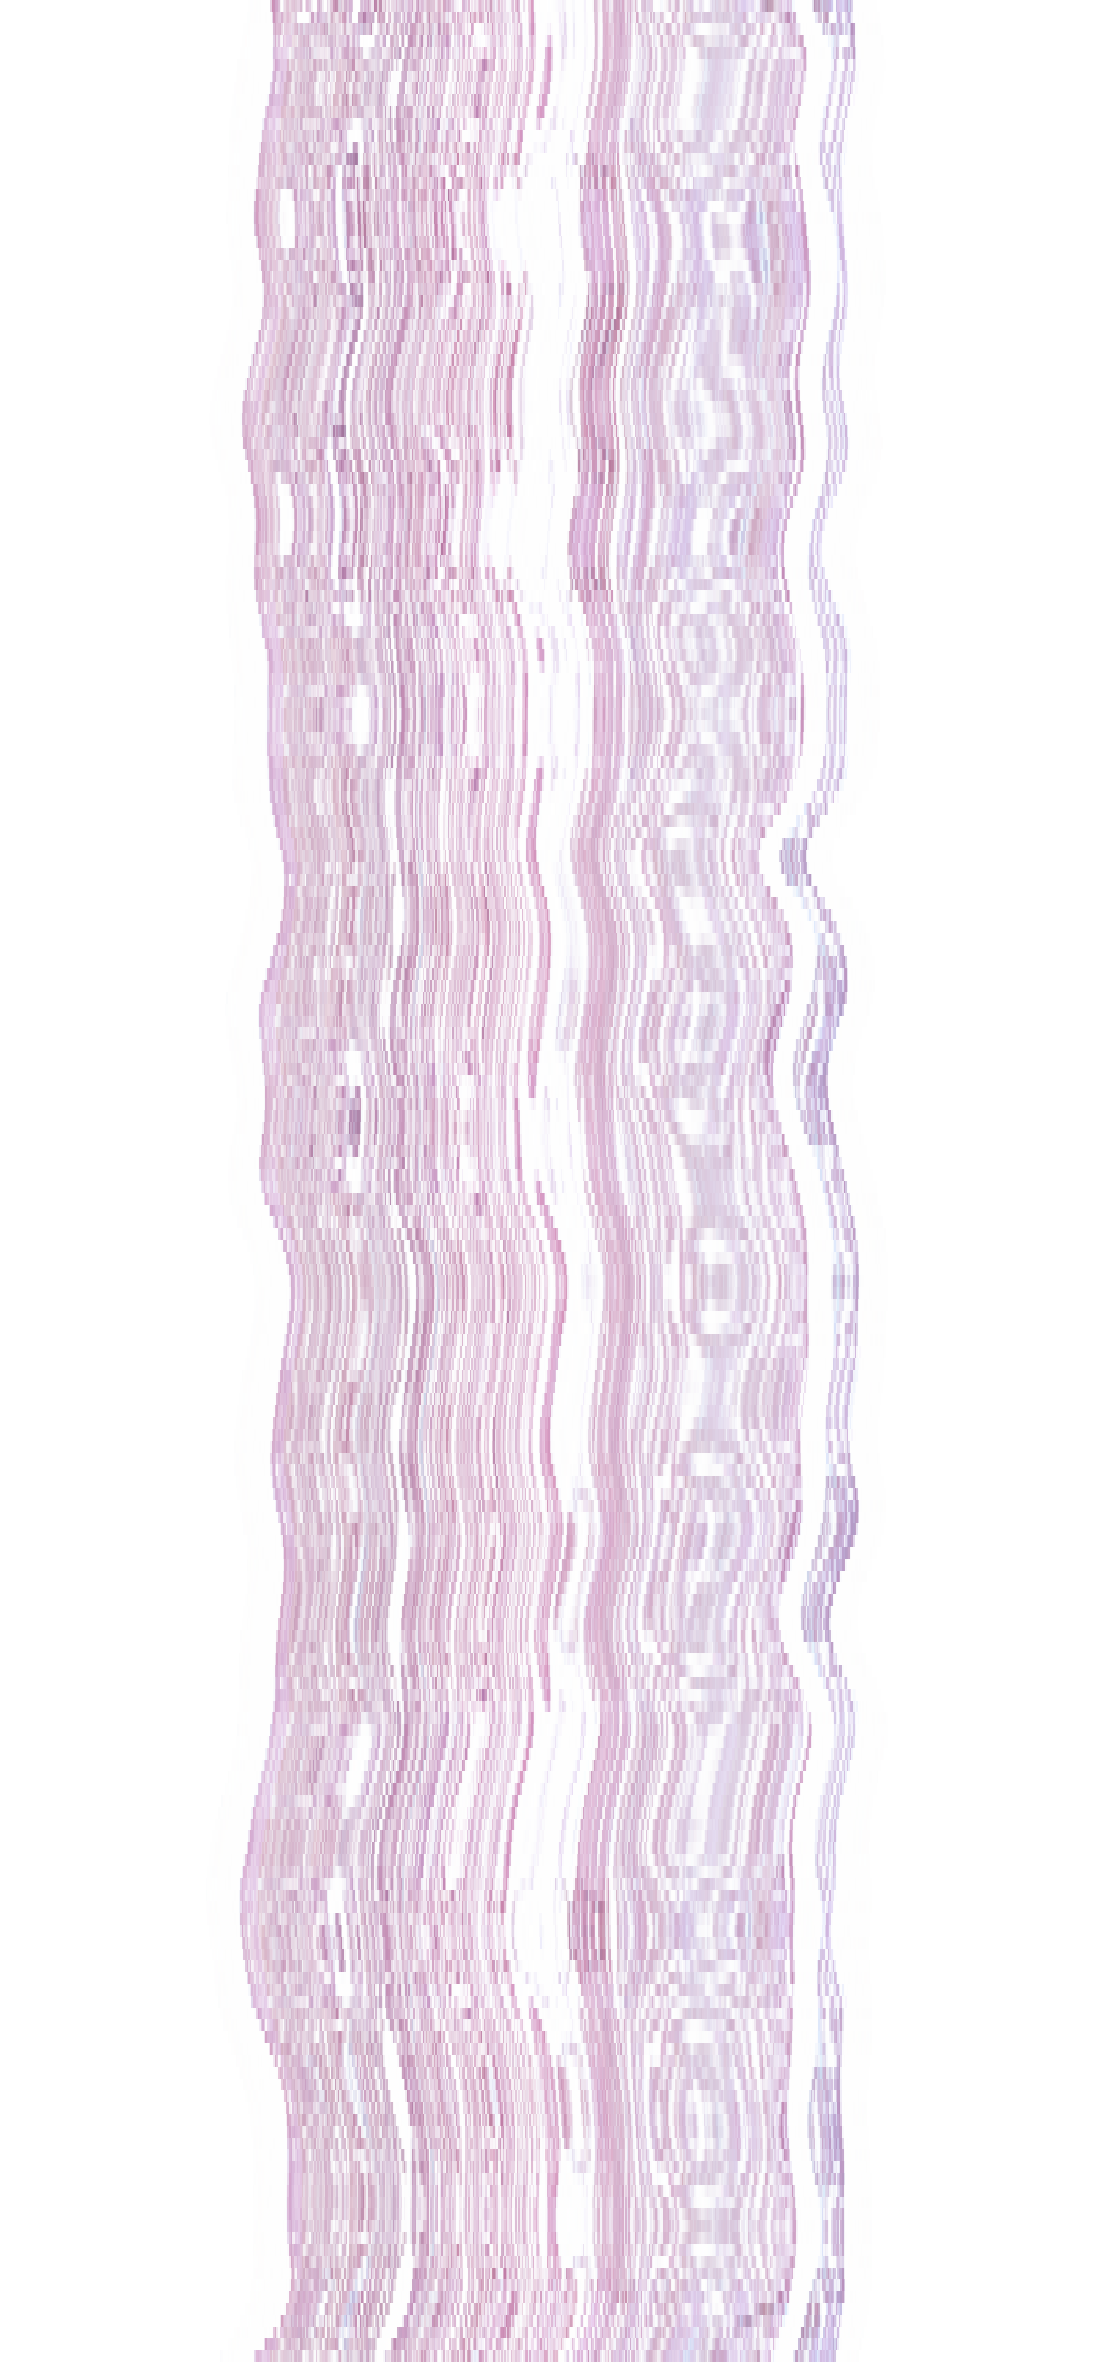
\includegraphics[height=0.4\textheight,type=pdf,ext=.pdf,read=.pdf]{Ch6/Figs/dummies/cross_section_200_alpha0.4_20_1_431}}
    \subfigure[][without noise]{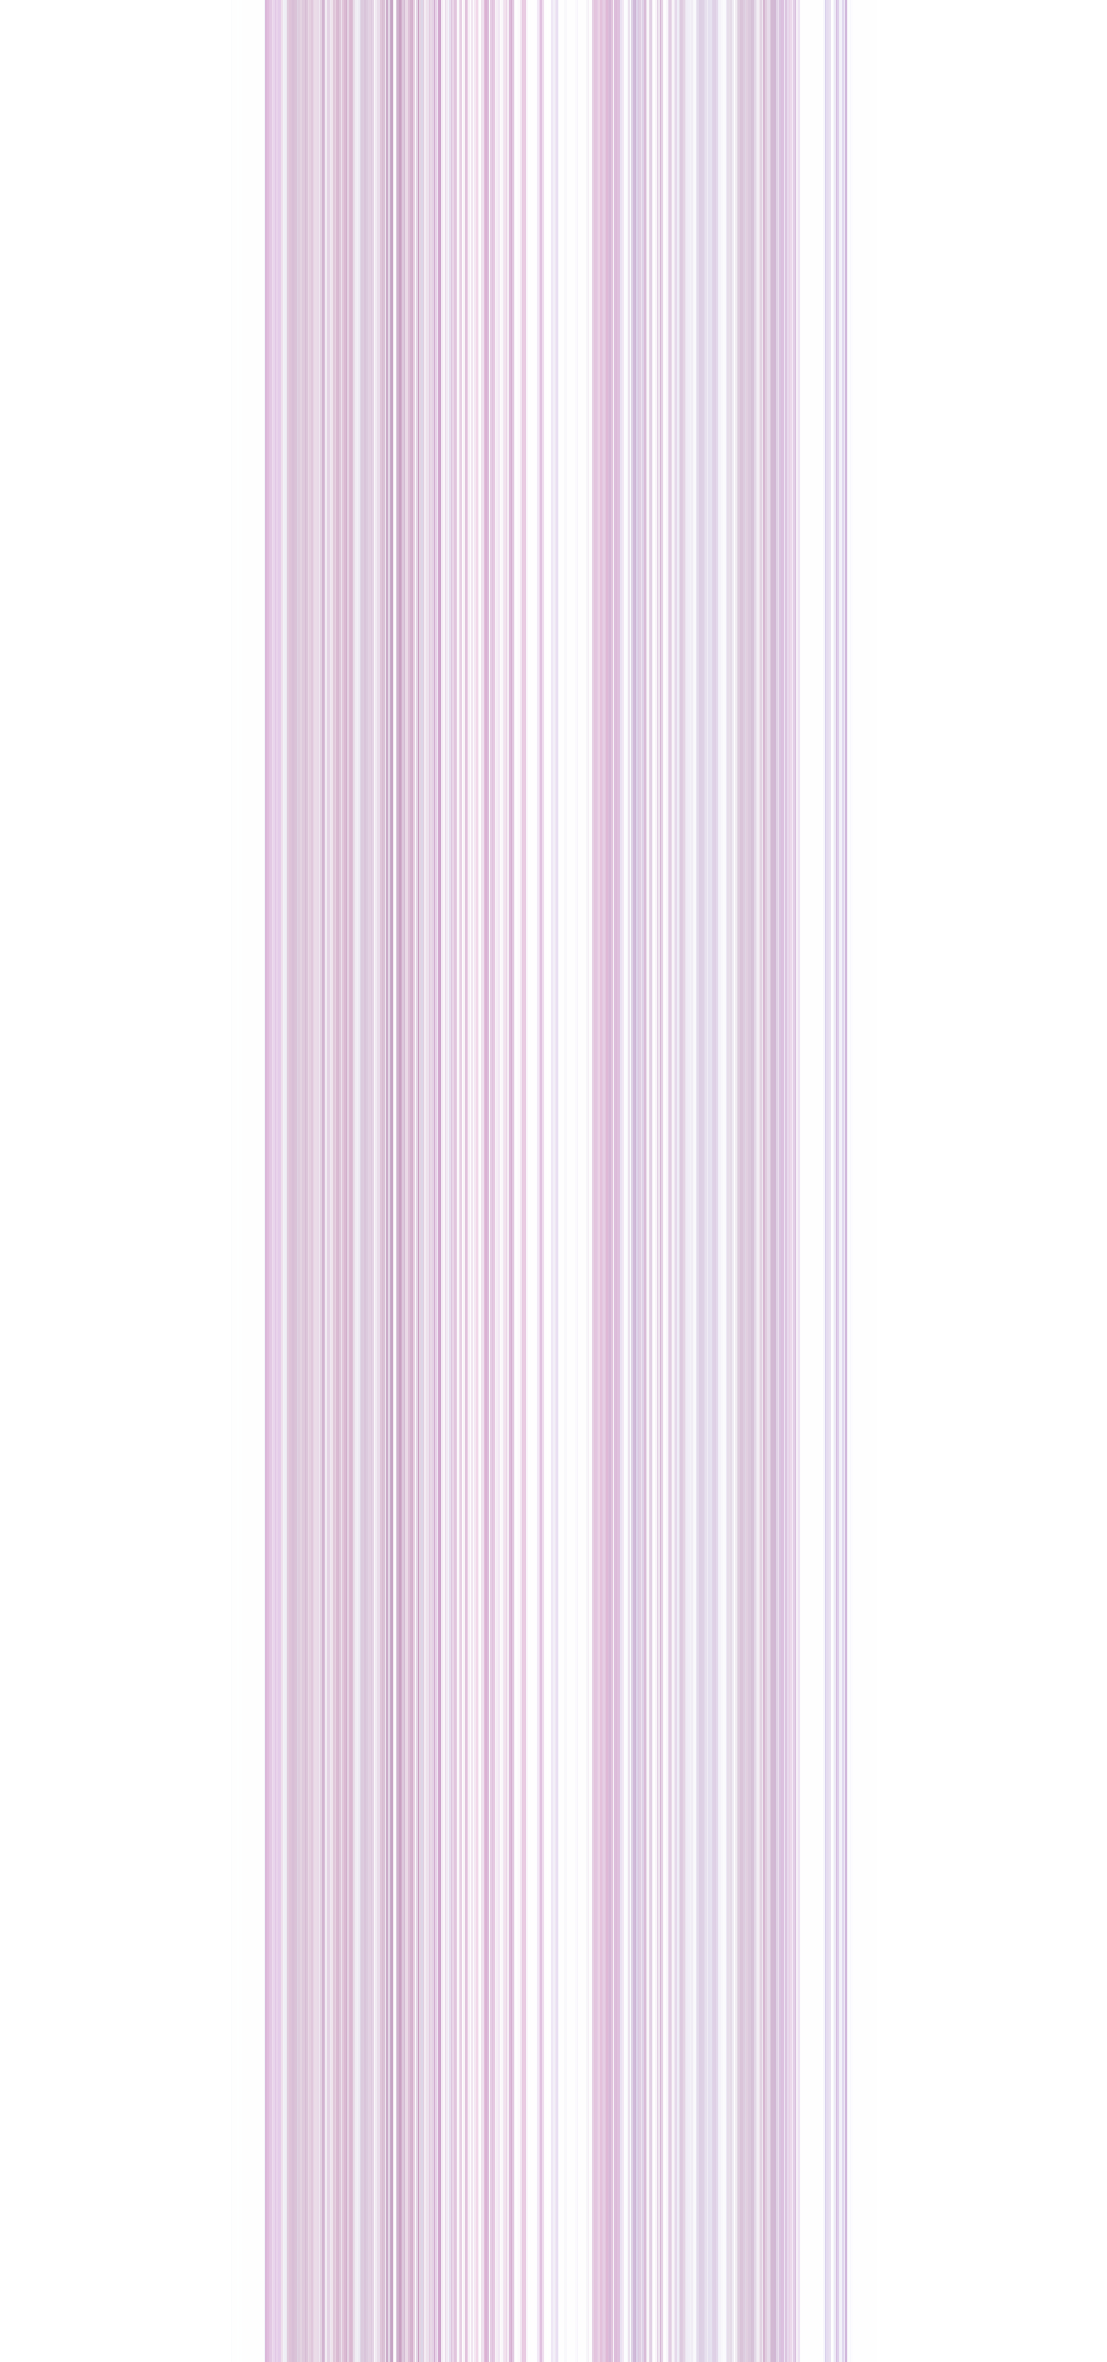
\includegraphics[height=0.4\textheight,type=pdf,ext=.pdf,read=.pdf]{Ch6/Figs/dummies/cross_section_perfect_200_alpha0.4_1_431}}
    \caption{Cross-sections of the straight volume, perpendicular to the y-axis.}
    \label{fig:cross_section_1}
  \end{figure}
    
  % rotated
  \begin{figure}[htbp]
    \centering
    \subfigure[][0 iterations]{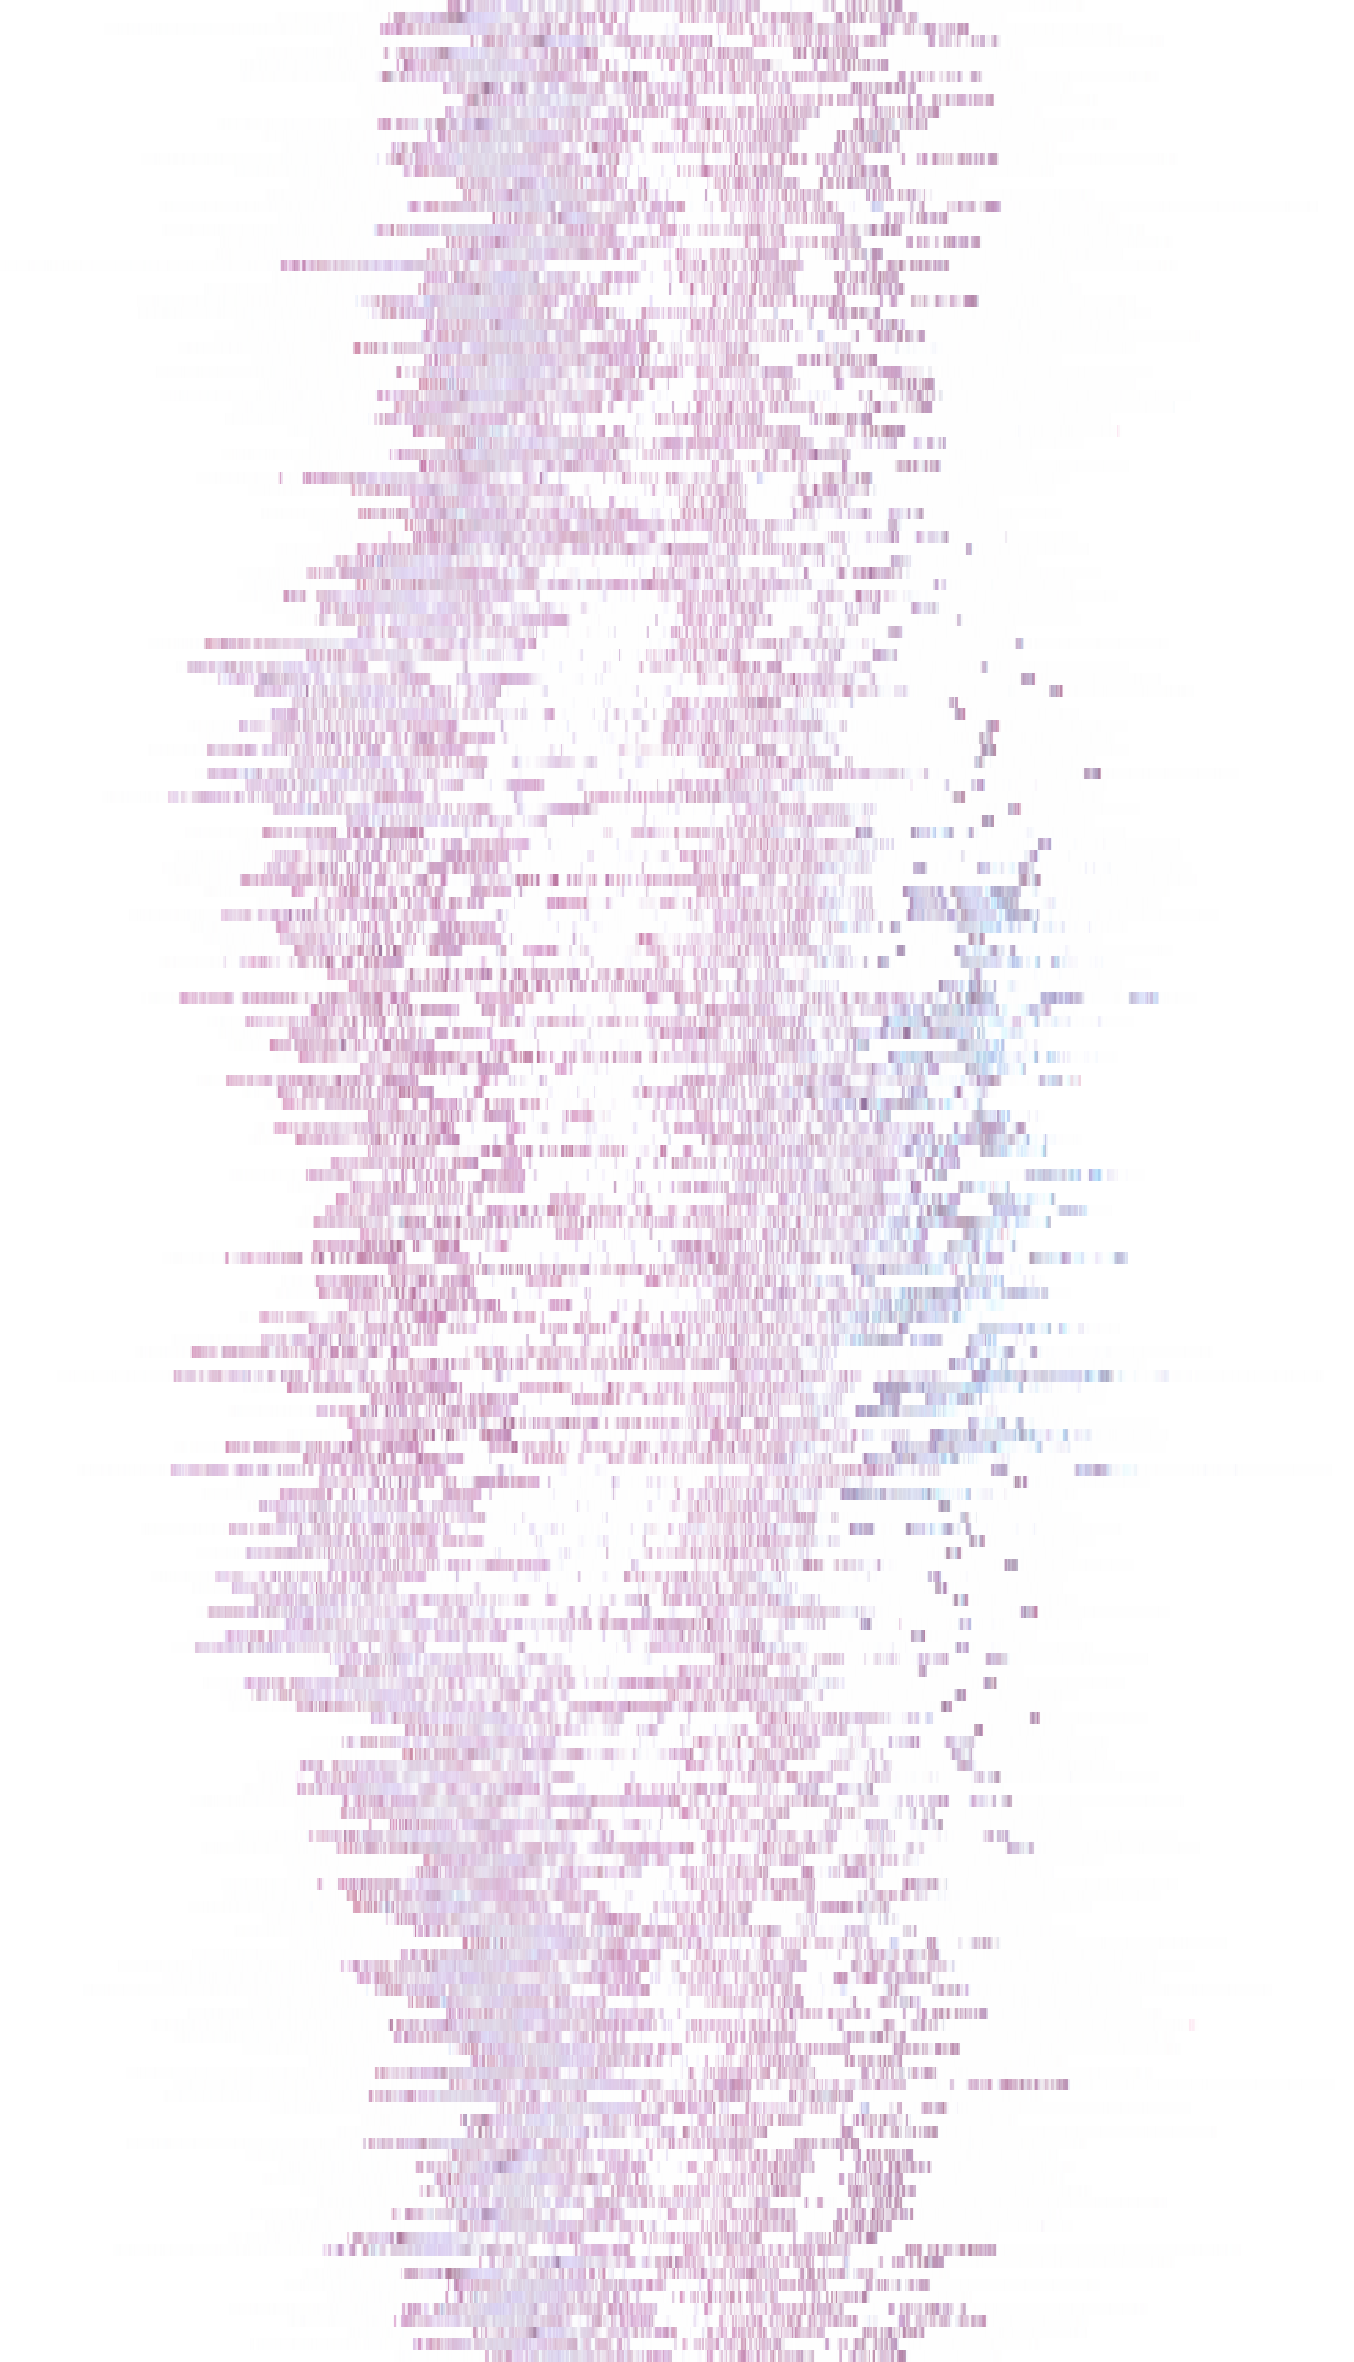
\includegraphics[height=0.4\textheight,type=pdf,ext=.pdf,read=.pdf]{Ch6/Figs/dummies/cross_section_200_alpha0.4r_0_0_352}}
    \subfigure[][1 iteration]{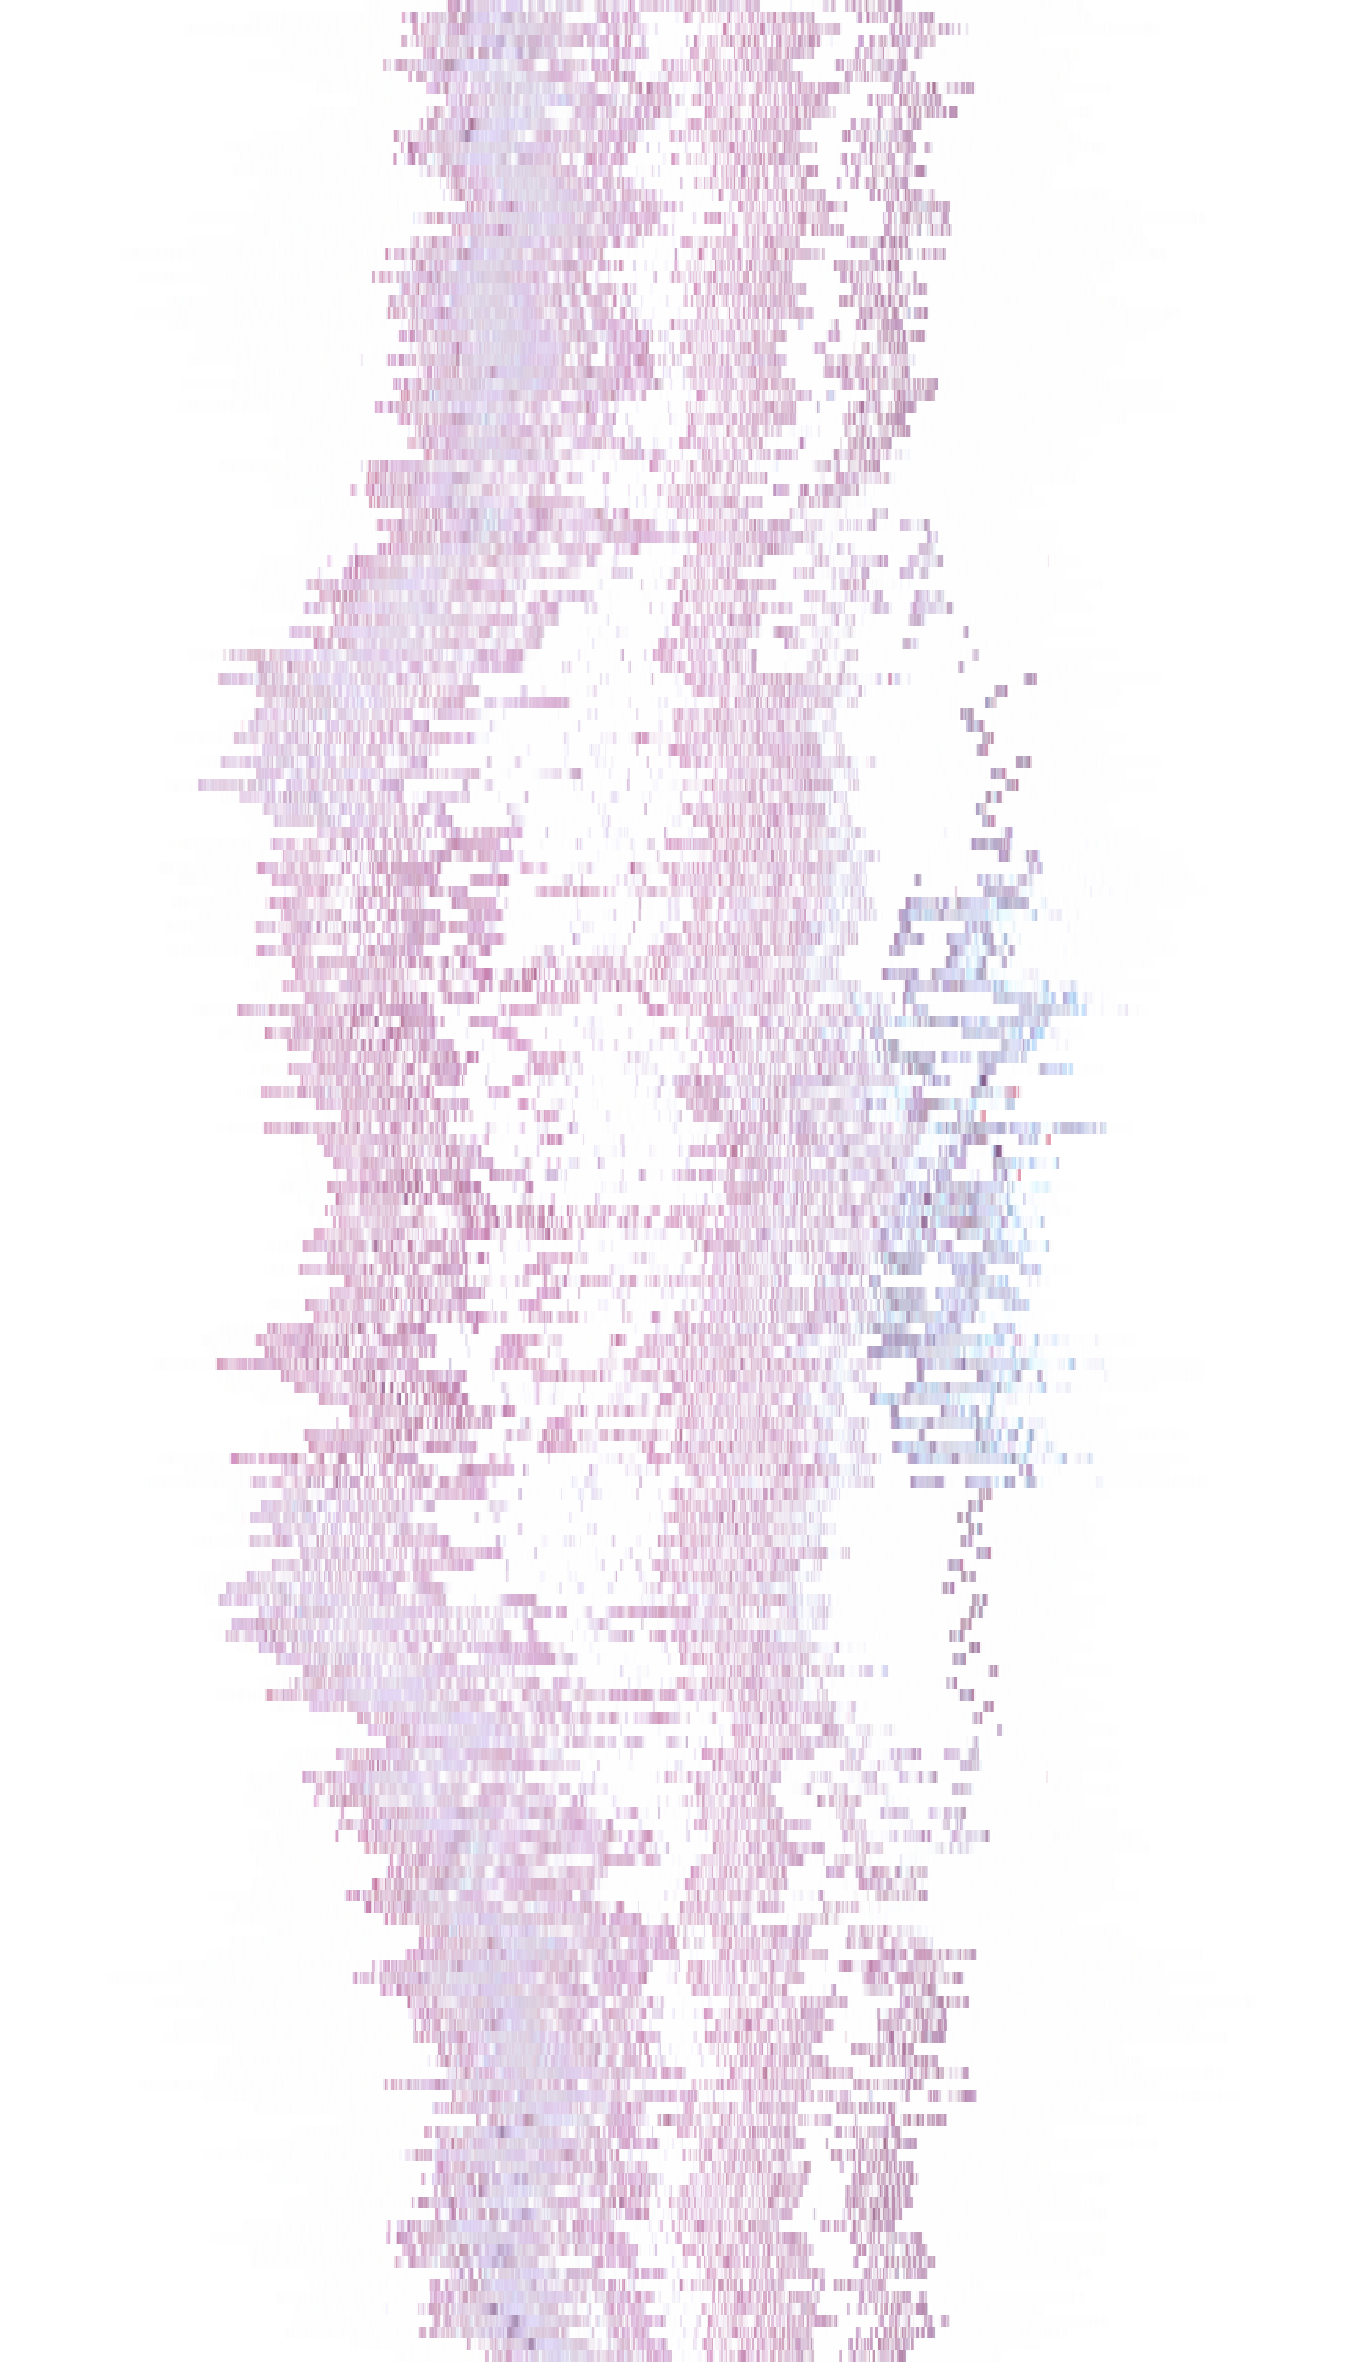
\includegraphics[height=0.4\textheight,type=pdf,ext=.pdf,read=.pdf]{Ch6/Figs/dummies/cross_section_200_alpha0.4r_1_0_352}}
    \subfigure[][3 iterations]{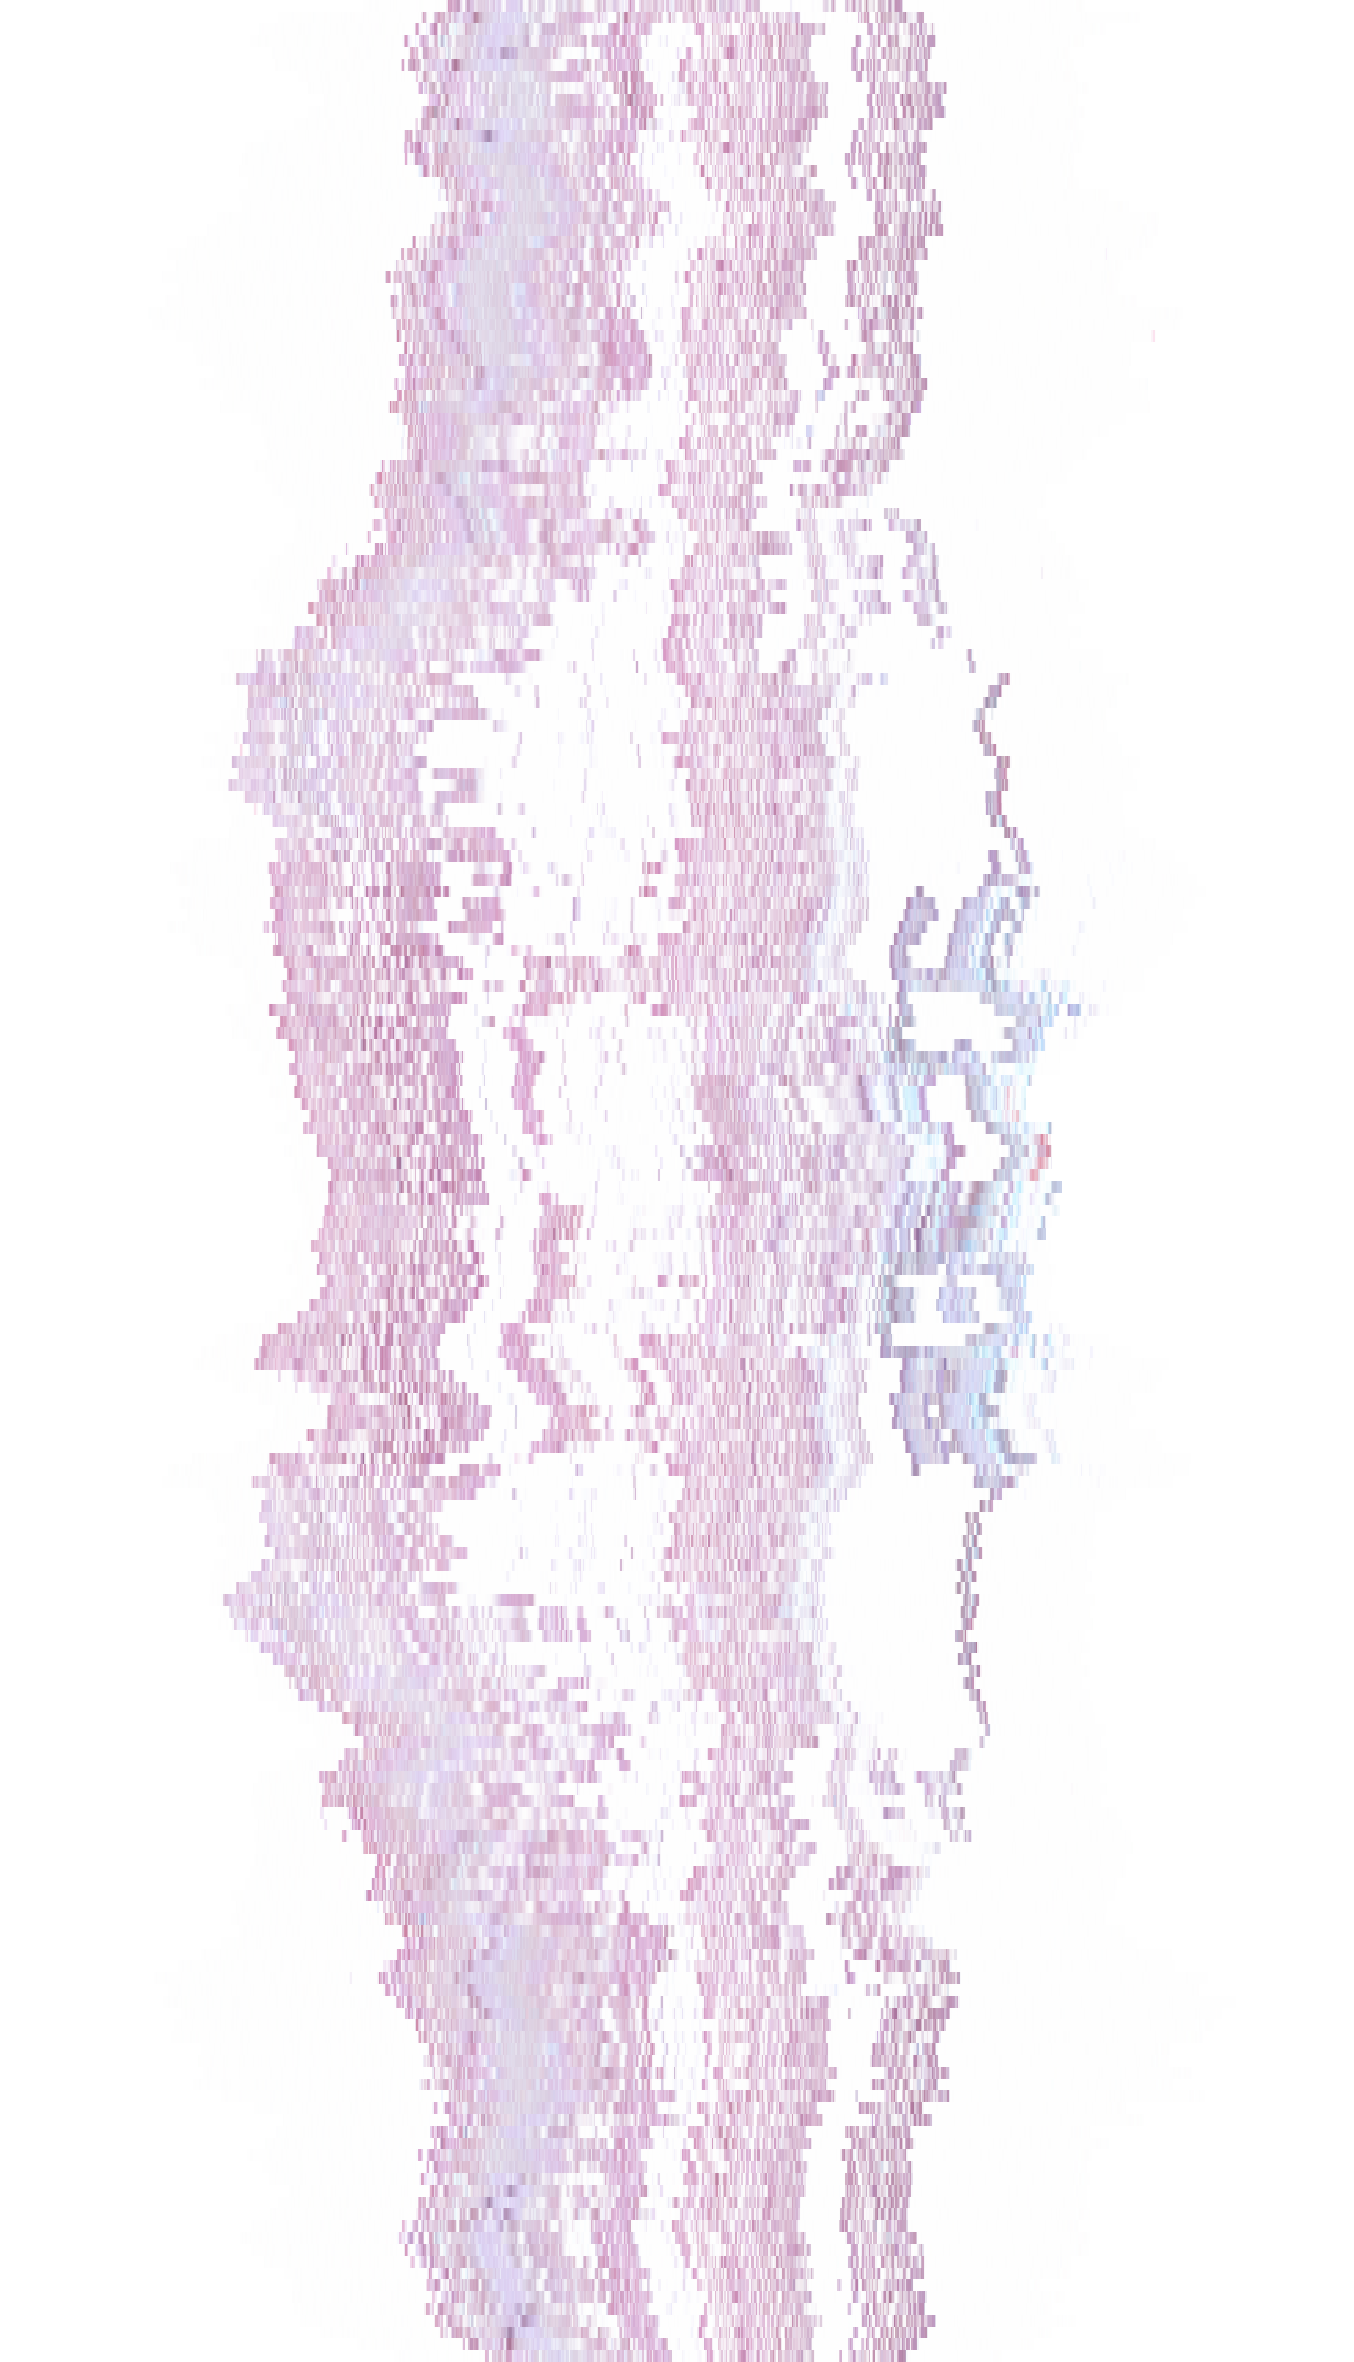
\includegraphics[height=0.4\textheight,type=pdf,ext=.pdf,read=.pdf]{Ch6/Figs/dummies/cross_section_200_alpha0.4r_3_0_352}}
    \subfigure[][8 iterations]{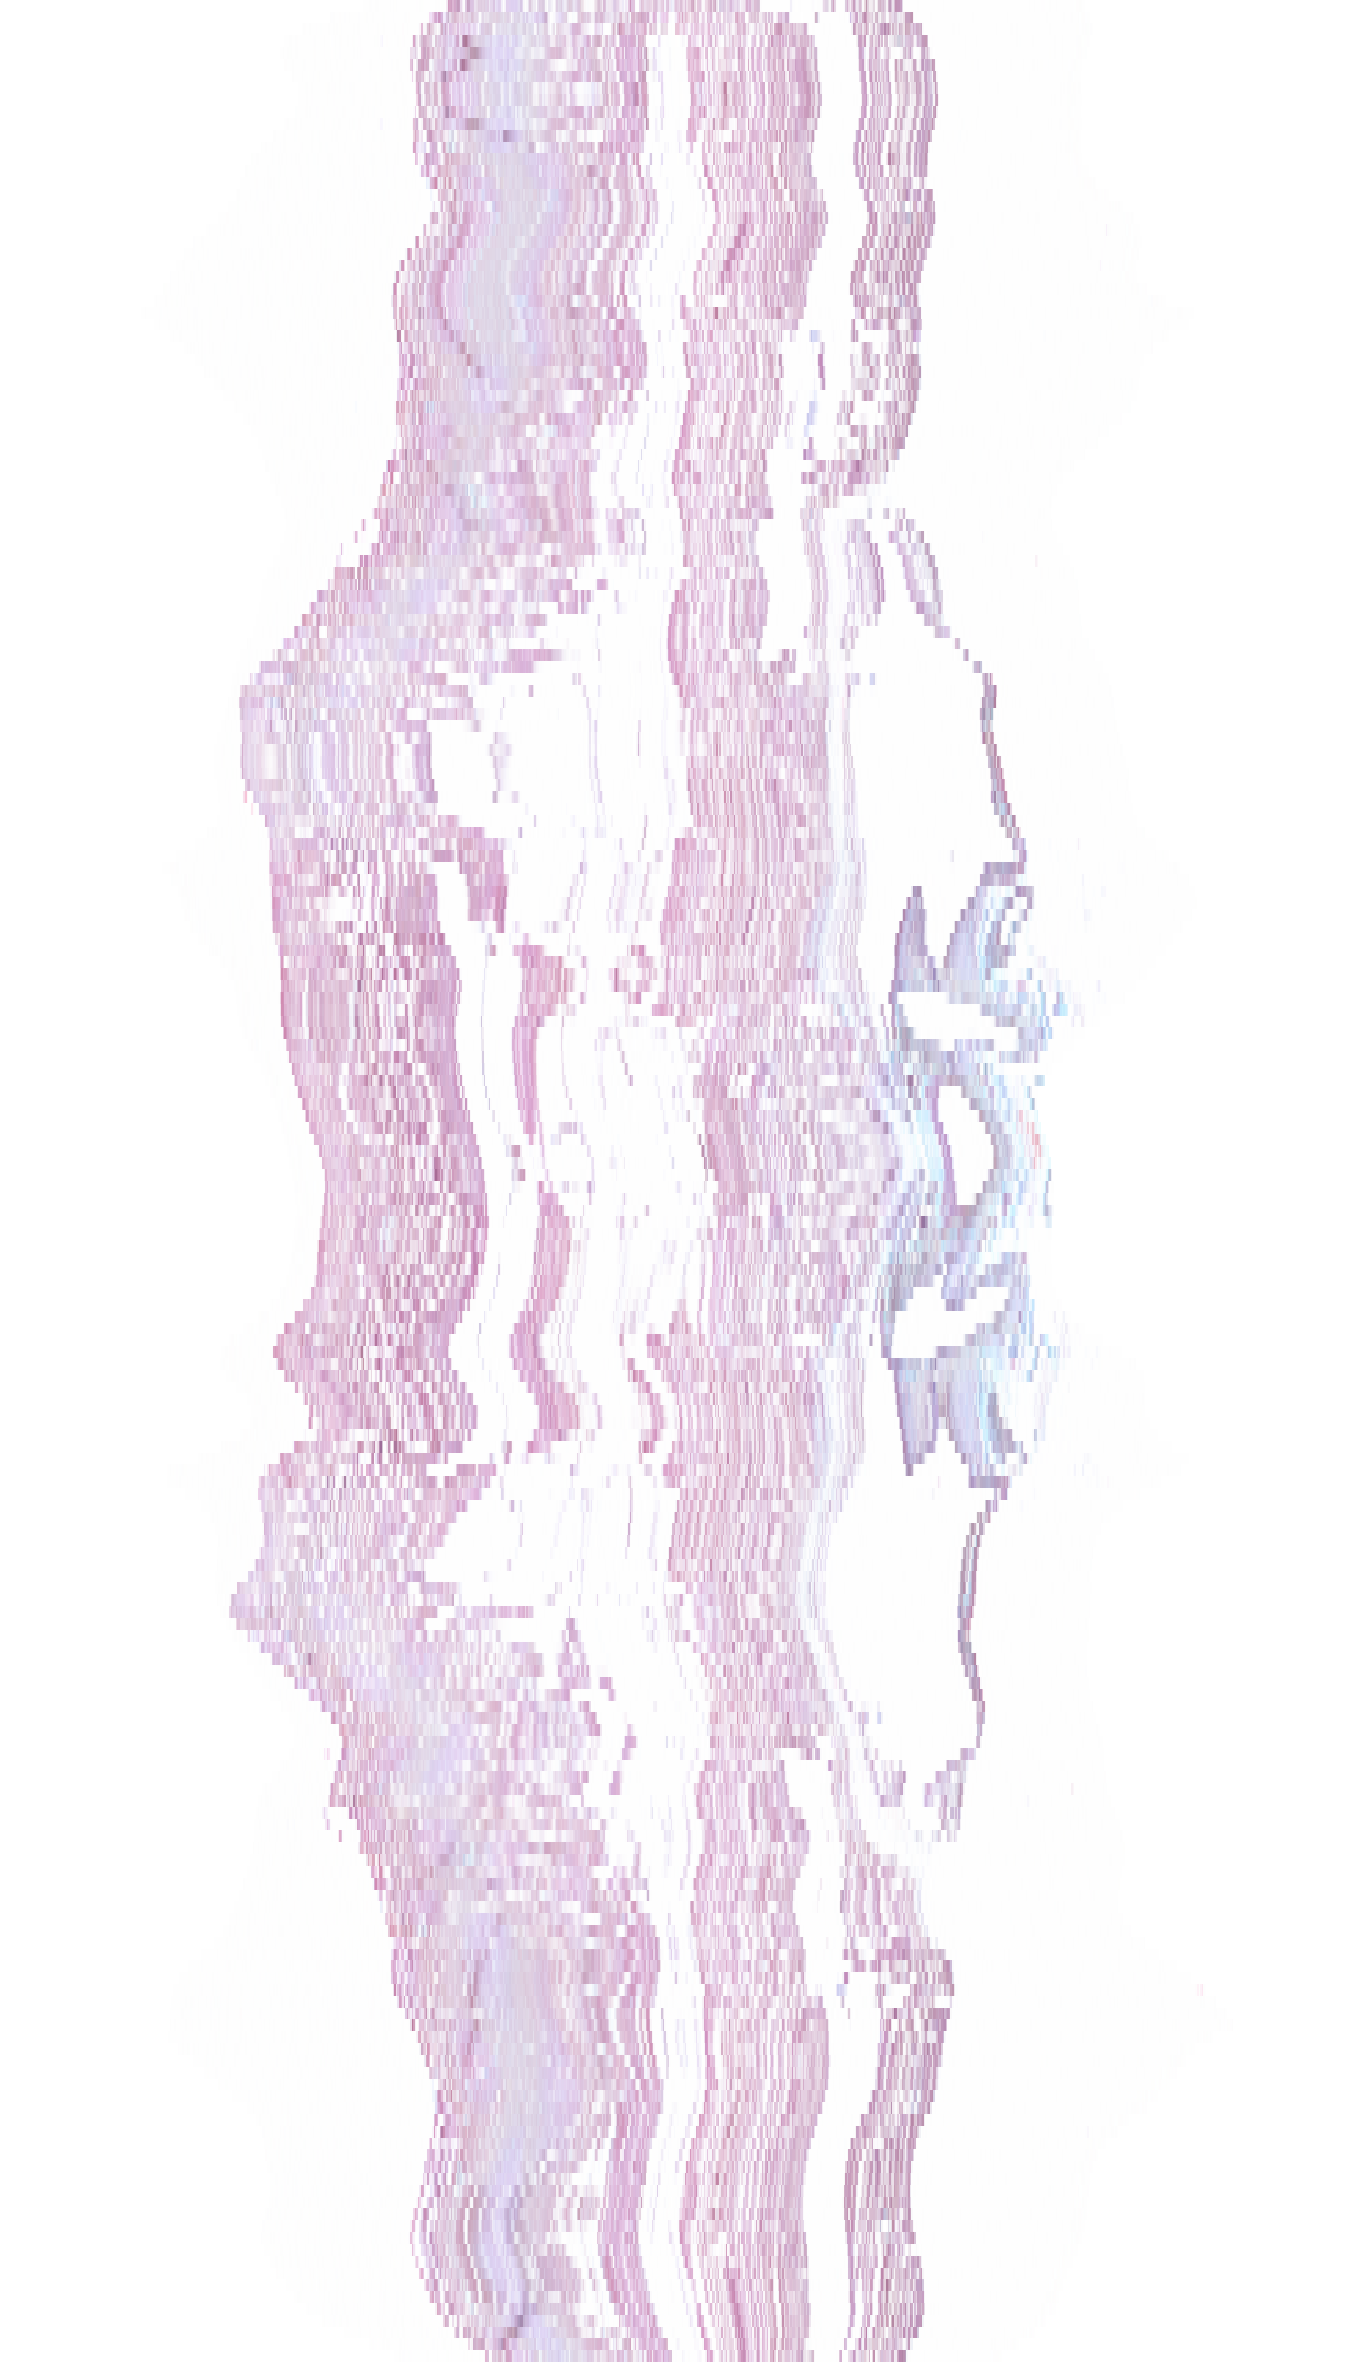
\includegraphics[height=0.4\textheight,type=pdf,ext=.pdf,read=.pdf]{Ch6/Figs/dummies/cross_section_200_alpha0.4r_8_0_352}}
    \subfigure[][20 iterations]{\includegraphics[height=0.4\textheight,type=pdf,ext=.pdf,read=.pdf]{Ch6/Figs/dummies/cross_section_200_alpha0.4r_20_0_352}}
    \subfigure[][without noise]{\includegraphics[height=0.4\textheight,type=pdf,ext=.pdf,read=.pdf]{Ch6/Figs/dummies/cross_section_perfect_200_alpha0.4r_0_352}}
    \caption{Cross-sections of the rotating volume, perpendicular to the x-axis.}
    \label{fig:cross_section_0r}
  \end{figure}
  
  \begin{figure}[htbp]
    \centering
    \subfigure[][0 iterations]{\includegraphics[height=0.4\textheight,type=pdf,ext=.pdf,read=.pdf]{Ch6/Figs/dummies/cross_section_200_alpha0.4r_0_1_431}}
    \subfigure[][1 iteration]{\includegraphics[height=0.4\textheight,type=pdf,ext=.pdf,read=.pdf]{Ch6/Figs/dummies/cross_section_200_alpha0.4r_1_1_431}}
    \subfigure[][3 iterations]{\includegraphics[height=0.4\textheight,type=pdf,ext=.pdf,read=.pdf]{Ch6/Figs/dummies/cross_section_200_alpha0.4r_3_1_431}}
    \subfigure[][8 iterations]{\includegraphics[height=0.4\textheight,type=pdf,ext=.pdf,read=.pdf]{Ch6/Figs/dummies/cross_section_200_alpha0.4r_8_1_431}}
    \subfigure[][20 iterations]{\includegraphics[height=0.4\textheight,type=pdf,ext=.pdf,read=.pdf]{Ch6/Figs/dummies/cross_section_200_alpha0.4r_20_1_431}}
    \subfigure[][without noise]{\includegraphics[height=0.4\textheight,type=pdf,ext=.pdf,read=.pdf]{Ch6/Figs/dummies/cross_section_perfect_200_alpha0.4r_1_431}}
    \caption{Cross-sections of the rotating volume, perpendicular to the y-axis.}
    \label{fig:cross_section_1r}
  \end{figure}
  
  % translated
  \begin{figure}[htbp]
    \centering
    \subfigure[][0 iterations]{\includegraphics[height=0.4\textheight,type=pdf,ext=.pdf,read=.pdf]{Ch6/Figs/dummies/cross_section_200_alpha0.4t_0_0_352}}
    \subfigure[][1 iteration]{\includegraphics[height=0.4\textheight,type=pdf,ext=.pdf,read=.pdf]{Ch6/Figs/dummies/cross_section_200_alpha0.4t_1_0_352}}
    \subfigure[][3 iterations]{\includegraphics[height=0.4\textheight,type=pdf,ext=.pdf,read=.pdf]{Ch6/Figs/dummies/cross_section_200_alpha0.4t_3_0_352}}
    \subfigure[][8 iterations]{\includegraphics[height=0.4\textheight,type=pdf,ext=.pdf,read=.pdf]{Ch6/Figs/dummies/cross_section_200_alpha0.4t_8_0_352}}
    \subfigure[][20 iterations]{\includegraphics[height=0.4\textheight,type=pdf,ext=.pdf,read=.pdf]{Ch6/Figs/dummies/cross_section_200_alpha0.4t_20_0_352}}
    \subfigure[][without noise]{\includegraphics[height=0.4\textheight,type=pdf,ext=.pdf,read=.pdf]{Ch6/Figs/dummies/cross_section_perfect_200_alpha0.4t_0_352}}
    \caption{Cross-sections of the translating volume, perpendicular to the x-axis.}
    \label{fig:cross_section_0t}
  \end{figure}
  
  \begin{figure}[htbp]
    \centering
    \subfigure[][0 iterations]{\includegraphics[height=0.4\textheight,type=pdf,ext=.pdf,read=.pdf]{Ch6/Figs/dummies/cross_section_200_alpha0.4t_0_1_431}}
    \subfigure[][1 iteration]{\includegraphics[height=0.4\textheight,type=pdf,ext=.pdf,read=.pdf]{Ch6/Figs/dummies/cross_section_200_alpha0.4t_1_1_431}}
    \subfigure[][3 iterations]{\includegraphics[height=0.4\textheight,type=pdf,ext=.pdf,read=.pdf]{Ch6/Figs/dummies/cross_section_200_alpha0.4t_3_1_431}}
    \subfigure[][8 iterations]{\includegraphics[height=0.4\textheight,type=pdf,ext=.pdf,read=.pdf]{Ch6/Figs/dummies/cross_section_200_alpha0.4t_8_1_431}}
    \subfigure[][20 iterations]{\includegraphics[height=0.4\textheight,type=pdf,ext=.pdf,read=.pdf]{Ch6/Figs/dummies/cross_section_200_alpha0.4t_20_1_431}}
    \subfigure[][without noise]{\includegraphics[height=0.4\textheight,type=pdf,ext=.pdf,read=.pdf]{Ch6/Figs/dummies/cross_section_perfect_200_alpha0.4t_1_431}}
    \caption{Cross-sections of the translating volume, perpendicular to the y-axis.}
    \label{fig:cross_section_1t}
  \end{figure}
    
  % rotated and translated
  \begin{figure}[htbp]
    \centering
    \subfigure[][0 iterations]{\includegraphics[height=0.4\textheight,type=pdf,ext=.pdf,read=.pdf]{Ch6/Figs/dummies/cross_section_200_alpha0.4rt_0_0_352}}
    \subfigure[][1 iteration]{\includegraphics[height=0.4\textheight,type=pdf,ext=.pdf,read=.pdf]{Ch6/Figs/dummies/cross_section_200_alpha0.4rt_1_0_352}}
    \subfigure[][3 iterations]{\includegraphics[height=0.4\textheight,type=pdf,ext=.pdf,read=.pdf]{Ch6/Figs/dummies/cross_section_200_alpha0.4rt_3_0_352}}
    \subfigure[][8 iterations]{\includegraphics[height=0.4\textheight,type=pdf,ext=.pdf,read=.pdf]{Ch6/Figs/dummies/cross_section_200_alpha0.4rt_8_0_352}}
    \subfigure[][20 iterations]{\includegraphics[height=0.4\textheight,type=pdf,ext=.pdf,read=.pdf]{Ch6/Figs/dummies/cross_section_200_alpha0.4rt_20_0_352}}
    \subfigure[][without noise]{\includegraphics[height=0.4\textheight,type=pdf,ext=.pdf,read=.pdf]{Ch6/Figs/dummies/cross_section_perfect_200_alpha0.4rt_0_352}}
    \caption{Cross-sections of the rotating and translating volume, perpendicular to the x-axis.}
    \label{fig:cross_section_0rt}
  \end{figure}
  
  \begin{figure}[htbp]
    \centering
    \subfigure[][0 iterations]{\includegraphics[height=0.4\textheight,type=pdf,ext=.pdf,read=.pdf]{Ch6/Figs/dummies/cross_section_200_alpha0.4rt_0_1_431}}
    \subfigure[][1 iteration]{\includegraphics[height=0.4\textheight,type=pdf,ext=.pdf,read=.pdf]{Ch6/Figs/dummies/cross_section_200_alpha0.4rt_1_1_431}}
    \subfigure[][3 iterations]{\includegraphics[height=0.4\textheight,type=pdf,ext=.pdf,read=.pdf]{Ch6/Figs/dummies/cross_section_200_alpha0.4rt_3_1_431}}
    \subfigure[][8 iterations]{\includegraphics[height=0.4\textheight,type=pdf,ext=.pdf,read=.pdf]{Ch6/Figs/dummies/cross_section_200_alpha0.4rt_8_1_431}}
    \subfigure[][20 iterations]{\includegraphics[height=0.4\textheight,type=pdf,ext=.pdf,read=.pdf]{Ch6/Figs/dummies/cross_section_200_alpha0.4rt_20_1_431}}
    \subfigure[][without noise]{\includegraphics[height=0.4\textheight,type=pdf,ext=.pdf,read=.pdf]{Ch6/Figs/dummies/cross_section_perfect_200_alpha0.4rt_1_431}}
    \caption{Cross-sections of the rotating and translating volume, perpendicular to the y-axis.}
    \label{fig:cross_section_1rt}
  \end{figure}
  
  The central cross-sections perpendicular to the x- and y-axes of the four regimes are exhibited in Figures~\labelcref{fig:cross_section_0,fig:cross_section_1,fig:cross_section_0r,fig:cross_section_1r,fig:cross_section_0t,fig:cross_section_1t,fig:cross_section_0rt,fig:cross_section_1rt}. The first section in each is of the original unsmoothed noisy volume, and the last of the volume before noise was added. Four images are sandwiched by these two extremes, of sections smoothed 1, 3, 8 and 20 times. The smoothing performs extremely well on two fronts. By iteration 20, a smooth, continuous section with the appearance of an original histology slice has been recovered from an unrecognisably noisy volume. Secondly and crucially, the underlying geometry of the tissue has been preserved, and the sections appear very similar to the ground truth sections before the noise had been added.
  
  % mean squared differences 3D
  \begin{sidewaysfigure}[htbp]
    \centering
    \subfigure[][straight column]{\includegraphics[height=0.33\textheight,type=pdf,ext=.pdf,read=.pdf]{Ch6/Figs/dummies/segmentation_mean_square_differences_3D}}
    \subfigure[][rotation]{\includegraphics[height=0.33\textheight,type=pdf,ext=.pdf,read=.pdf]{Ch6/Figs/dummies/segmentation_mean_square_differences_3Dr}}
    \subfigure[][translation]{\includegraphics[height=0.33\textheight,type=pdf,ext=.pdf,read=.pdf]{Ch6/Figs/dummies/segmentation_mean_square_differences_3Dt}}
    \subfigure[][rotation and translation]{\includegraphics[height=0.33\textheight,type=pdf,ext=.pdf,read=.pdf]{Ch6/Figs/dummies/segmentation_mean_square_differences_3Drt}}
    \caption{The 3D evolution of mean squared pixel intensity differences between adjacent slices for each of the four geometrical regimes.}
    \label{fig:mean_squared_differences_3D}
  \end{sidewaysfigure}
  
  Registration was performed using the mean square difference metric, and Figure~\ref{fig:mean_squared_differences_3D} graphs the evolving mean squared pixel intensity difference between each slice and its successor after repeated applications of the smoothing algorithm. In all four geometrical regimes, and for all slices away from the boundaries, the metric is greatly reduced, evidence that each slice is much more closely aligned with its neighbours. Just as in the case of 1D diffusion, most of the reduction is yielded in the earlier iterations, when the highest frequencies are damped most easily. Registrations were verified to be successful in the overwhelming majority of cases, ending with an oscillation around a consistent, very low mean squared difference value.
  
  % mean squared differences 2D
  \begin{sidewaysfigure}[htbp]
    \centering
    \subfigure[][straight column]{\includegraphics[height=0.33\textheight,type=pdf,ext=.pdf,read=.pdf]{Ch6/Figs/dummies/segmentation_mean_square_differences_2D}}
    \subfigure[][rotation]{\includegraphics[height=0.33\textheight,type=pdf,ext=.pdf,read=.pdf]{Ch6/Figs/dummies/segmentation_mean_square_differences_2Dr}}
    \subfigure[][translation]{\includegraphics[height=0.33\textheight,type=pdf,ext=.pdf,read=.pdf]{Ch6/Figs/dummies/segmentation_mean_square_differences_2Dt}}
    \subfigure[][rotation and translation]{\includegraphics[height=0.33\textheight,type=pdf,ext=.pdf,read=.pdf]{Ch6/Figs/dummies/segmentation_mean_square_differences_2Drt}}
    \caption{The initial (blue) and final (green) mean squared pixel intensities between adjacent pairs for each of the four geometrical regimes.}
    \label{fig:mean_squared_differences_2D}
  \end{sidewaysfigure}

  Figure~\ref{fig:mean_squared_differences_2D} graphs the initial and final metric values between adjacent pairs for the four test regimes. Note that each blue (resp. green) line is equivalent to the starting values on the left (resp. right) face of the corresponding plot in Figure~\ref{fig:mean_squared_differences_3D}. Almost ubiquitously, the value is substantially lower after transformational diffusion, with the green lines appearing much smoother after the high frequency spectrum has been preferentially damped.
  
  There is one notable example of a registration that has failed to reach a good alignment, manifested in Figure~\ref{fig:mean_squared_differences_3D}~\textbf{(a)} as a large spike in the metric value of slice 152 at iteration 6. The deviation is also visible in Figures~\labelcref{fig:cross_section_0,fig:cross_section_1}~\textbf{(d)} at iteration 8, as a large displacement two thirds of the way up from the base. At each iteration of the algorithm, the slices have moved relative to each other, and hence are initialised outside of any preceding local minimum trap. In this way, all adjacent slices are given multiple chances to become aligned, conferring to this method a great deal of robustness not present in any previous technique in the literature. By iteration 20 in Figures~\labelcref{fig:cross_section_0,fig:cross_section_1}~\textbf{(d)}, the aberration is imperceptible, and we can see from Figure~\ref{fig:mean_squared_differences_3D}~\textbf{(a)} that the erroneous metric value has returned to a level comparable with its neighbours after just four iterations.
  
  % full contours
  \begin{figure}[htbp]\texttt{}
    \centering
    \subfigure[][0 iterations]{\includegraphics[width=0.3\pagewidth]{Ch6/Figs/dummies/contours/whole_surface_0}}
    \subfigure[][1 iteration]{\includegraphics[width=0.3\pagewidth]{Ch6/Figs/dummies/contours/whole_surface_1}}
    \subfigure[][3 iterations]{\includegraphics[width=0.3\pagewidth]{Ch6/Figs/dummies/contours/whole_surface_3}}
    \subfigure[][8 iterations]{\includegraphics[width=0.3\pagewidth]{Ch6/Figs/dummies/contours/whole_surface_8}}
    \subfigure[][20 iterations]{\includegraphics[width=0.3\pagewidth]{Ch6/Figs/dummies/contours/whole_surface_20}}
    \caption{Isosurfaces of the perturbed straight volume in red at several stages of smoothing, overlayed with the unperturbed volume in green.}
    \label{fig:dummy_contour}
  \end{figure}
  
  \begin{figure}[htbp]
    \centering
    \subfigure[][0 iterations]{\includegraphics[width=0.3\pagewidth]{Ch6/Figs/dummies/contours/whole_surfacer_0}}
    \subfigure[][1 iteration]{\includegraphics[width=0.3\pagewidth]{Ch6/Figs/dummies/contours/whole_surfacer_1}}
    \subfigure[][3 iterations]{\includegraphics[width=0.3\pagewidth]{Ch6/Figs/dummies/contours/whole_surfacer_3}}
    \subfigure[][8 iterations]{\includegraphics[width=0.3\pagewidth]{Ch6/Figs/dummies/contours/whole_surfacer_8}}
    \subfigure[][20 iterations]{\includegraphics[width=0.3\pagewidth]{Ch6/Figs/dummies/contours/whole_surfacer_20}}
    \caption{Isosurfaces of the rotating volume.}
    \label{fig:dummy_contourr}
  \end{figure}
  
  \begin{figure}[htbp]
    \centering
    \subfigure[][0 iterations]{\includegraphics[width=0.3\pagewidth]{Ch6/Figs/dummies/contours/whole_surfacet_0}}
    \subfigure[][1 iteration]{\includegraphics[width=0.3\pagewidth]{Ch6/Figs/dummies/contours/whole_surfacet_1}}
    \subfigure[][3 iterations]{\includegraphics[width=0.3\pagewidth]{Ch6/Figs/dummies/contours/whole_surfacet_3}}
    \subfigure[][8 iterations]{\includegraphics[width=0.3\pagewidth]{Ch6/Figs/dummies/contours/whole_surfacet_8}}
    \subfigure[][20 iterations]{\includegraphics[width=0.3\pagewidth]{Ch6/Figs/dummies/contours/whole_surfacet_20}}
    \caption{Isosurfaces of the translating volumes.}
    \label{fig:dummy_contourt}
  \end{figure}
  
  \begin{figure}[htbp]
    \centering
    \subfigure[][0 iterations]{\includegraphics[width=0.3\pagewidth]{Ch6/Figs/dummies/contours/whole_surfacert_0}}
    \subfigure[][1 iteration]{\includegraphics[width=0.3\pagewidth]{Ch6/Figs/dummies/contours/whole_surfacert_1}}
    \subfigure[][3 iterations]{\includegraphics[width=0.3\pagewidth]{Ch6/Figs/dummies/contours/whole_surfacert_3}}
    \subfigure[][8 iterations]{\includegraphics[width=0.3\pagewidth]{Ch6/Figs/dummies/contours/whole_surfacert_8}}
    \subfigure[][20 iterations]{\includegraphics[width=0.3\pagewidth]{Ch6/Figs/dummies/contours/whole_surfacert_20}}
    \caption{Isosurfaces of the translating and rotating volumes.}
    \label{fig:dummy_contourrt}
  \end{figure}
  
  The nature of the 3D geometry of the volumes --- the rotation and translation signals, and the transformational noise --- is most clearly understood from the segmentation volume isosurfaces in Figures~\labelcref{fig:dummy_contour,fig:dummy_contourr,fig:dummy_contourt,fig:dummy_contourrt}. Each of the 5 levels of smoothing depicted by Figures~\labelcref{fig:cross_section_0,fig:cross_section_1,fig:cross_section_0r,fig:cross_section_1r,fig:cross_section_0t,fig:cross_section_1t,fig:cross_section_0rt,fig:cross_section_1rt} are overlayed in red with their equivalent unperturbed volumes in green. Again, the smoothing brings the noisy volume much more closely in line with the ground truth, with the largest effect on the higher frequencies of noise. The conservation of the underlying structure is most evident in Figure~\ref{fig:dummy_contourrt}~(e), where the red isosurface deviates almost imperceptibly from the green.
  
  Parameters used in the registration are listed in Table~\ref{tab:dummy_histo_to_histo}. It is worth noting that as long as the registration process is refined enough to arrive dependably near the global minimum, the adjustment algorithm itself is stable with much larger levels of noise than showcased here. For example, one approach might be to preprocess images and tune parameters to cope with large displacements for the first few smoothing iterations, and then tune for smaller displacements during the finer smoothing in the later iterations. Yet, this kind of approach requires heavy manual intervention, and is highly specific to the problem at hand.
  % subsection simulating_transformational_diffusion (end)
% section methods (end)

\section{Results} % (fold)
\label{sec:results}
  \subsection{Global Diffusion} % (fold)
  \label{sub:global_diffusion}
    % x slices
    \begin{figure}[htbp]
      \centering
      \subfigure[][0 iterations (unsmoothed affine volume)]{\includegraphics[height=0.31\textheight]{Ch6/Figs/adjusted_0_0_235}}
      \subfigure[][1 iteration]{\includegraphics[height=0.31\textheight]{Ch6/Figs/adjusted_1_0_235}}
      \subfigure[][20 iterations]{\includegraphics[height=0.31\textheight]{Ch6/Figs/adjusted_20_0_235}}
      \caption{Cross-sections of the full Rat28 volume perpendicular to the x-axis, after 0, 1 and 20 iterations of diffusion. The yellow boxes highlight the zoomed regions in Figure~\ref{fig:adjusted_bottom_vessels_0_235}.}
      \label{fig:adjusted_0_235}
    \end{figure}

    % y slices
    \begin{figure}[htbp]
      \centering
      \subfigure[][0 iterations (unsmoothed affine volume)]{\includegraphics[height=0.31\textheight]{Ch6/Figs/adjusted_0_1_287}}
      \subfigure[][1 iteration]{\includegraphics[height=0.31\textheight]{Ch6/Figs/adjusted_1_1_287}}
      \subfigure[][20 iterations]{\includegraphics[height=0.31\textheight]{Ch6/Figs/adjusted_20_1_287}}
      \caption{Cross-sections of the full Rat28 volume perpendicular to the y-axis, after 0, 1 and 20 iterations of diffusion. The yellow boxes highlight the zoomed regions in Figure~\ref{fig:adjusted_bottom_vessels_1_287}.}
      \label{fig:adjusted_1_287}
    \end{figure}
    
    20 iterations of smoothing were applied to the affine registered full-heart volume from Section~\ref{sec:registration_results}, and Figures~\labelcref{fig:adjusted_0_235,fig:adjusted_1_287} compare the central cross-sections of the volume before smoothing, after 1 iteration and after all 20 iterations. A subtle, but unmistakable improvement in coherence is observed; internal and external edges are smoother, especially towards the extremities of the heart, and clear, waving sheet structure has emerged, previously indistinguishable beyond the high-frequency zig-zagging noise.
    
    % lower 100 slices zoom
    % x slices
    \begin{sidewaysfigure}[htbp]
      \centering
      \subfigure[][0 iterations (unsmoothed affine volume)]{\includegraphics[height=0.12\textheight]{Ch6/Figs/adjusted_0_0_235_zoomed}}
      \subfigure[][1 iteration]{\includegraphics[height=0.12\textheight]{Ch6/Figs/adjusted_1_0_235_zoomed}}
      \subfigure[][20 iterations]{\includegraphics[height=0.12\textheight]{Ch6/Figs/adjusted_20_0_235_zoomed}}
      \caption{Cross-sections of the lower 100 slices perpendicular to the x-axis. The blue arrows highlight blue-stained interstitial tissue around vessels, the green arrow epicardial vessels and the yellow arrow enhanced sheet structure.}
      \label{fig:adjusted_bottom_vessels_0_235}
    \end{sidewaysfigure}

    % y slices
    \begin{sidewaysfigure}[htbp]
      \centering
      \subfigure[][0 iterations (unsmoothed affine volume)]{\includegraphics[height=0.12\textheight]{Ch6/Figs/adjusted_0_1_287_zoomed}}
      \subfigure[][1 iteration]{\includegraphics[height=0.12\textheight]{Ch6/Figs/adjusted_1_1_287_zoomed}}
      \subfigure[][20 iterations]{\includegraphics[height=0.12\textheight]{Ch6/Figs/adjusted_20_1_287_zoomed}}
      \caption{Cross-sections of the lower 100 slices perpendicular to the y-axis. The green arrows highlight epicardial vessels and the yellow arrow enhanced sheet structure.}
      \label{fig:adjusted_bottom_vessels_1_287}
    \end{sidewaysfigure}
    
    The effect is clearer in an enlargement of the bottom 100 slices in Figures~\labelcref{fig:adjusted_bottom_vessels_0_235,fig:adjusted_bottom_vessels_1_287}. The outer walls are several orders of magnitude less noisy in both figures, and internal vessel walls are much more coherent, most notably the epicardial vessels on the left and right of Figure~\ref{fig:adjusted_bottom_vessels_1_287}~(c). Sheet structure that started to surface from obscurity after just one iteration has been well resolved after 20 iterations. Figures~\labelcref{fig:whole_positive_x_diffused,fig:whole_negative_x_diffused,fig:whole_positive_y_diffused,fig:whole_positive_z_diffused} depict the smoother global contour after 20 iterations from several angles.
    
    % diffused contours
    \begin{sidewaysfigure}[p]
      \centering
      \includegraphics[width=0.9\textheight]{Ch6/Figs/Rat28/contours/whole_positive_x_diffused}
      \caption{Globally smoothed slice volume, viewed along the positive x direction.}
      \label{fig:whole_positive_x_diffused}
    \end{sidewaysfigure}

    \begin{sidewaysfigure}[p]
      \centering
      \includegraphics[width=0.9\textheight]{Ch6/Figs/Rat28/contours/whole_positive_z_diffused}
      \caption{Globally smoothed slice volume, viewed along the positive z direction.}
      \label{fig:whole_positive_z_diffused}
    \end{sidewaysfigure}
  % subsection global_diffusion (end)
  
  \subsection{Regional Diffusion} % (fold)
  \label{sub:regional_diffusion}
    \begin{figure}[p]
      \centering
      \subfigure[][Original block face registration]{\includegraphics[height=0.21\textheight]{Ch6/Figs/bottom_vessels/unsmoothed_vessel_0_2875}}
      \subfigure[][Globally smoothed registration]{\includegraphics[height=0.21\textheight]{Ch6/Figs/bottom_vessels/globally_smoothed_vessel_0_2875}}
      \subfigure[][Regionally smoothed registration]{\includegraphics[height=0.21\textheight]{Ch6/Figs/bottom_vessels/regionally_smoothed_vessel_0_2875}}
      \caption{Central cross sections of the region around an epicardial vessel, perpendicular to the x axis. Cross-sections are compared before smoothing, after global smoothing and after smoothing applied to this region. The blue arrow highlights blue-stained interstitial tissue around vessels, the green arrow epicardial vessels and the yellow arrow enhanced sheet structure.}
      \label{fig:vessel_cross_section_x}
    \end{figure}
    
    \begin{figure}[p]
      \centering
      \subfigure[][Original block face registration]{\includegraphics[height=0.21\textheight]{Ch6/Figs/bottom_vessels/unsmoothed_vessel_1_2125}}
      \subfigure[][Globally smoothed registration]{\includegraphics[height=0.21\textheight]{Ch6/Figs/bottom_vessels/globally_smoothed_vessel_1_2125}}
      \subfigure[][Regionally smoothed registration]{\includegraphics[height=0.21\textheight]{Ch6/Figs/bottom_vessels/regionally_smoothed_vessel_1_2125}}
      \caption{Central cross sections of the region around an epicardial vessel, perpendicular to the y axis.  The blue arrow highlights blue-stained interstitial tissue around vessels, the green arrow epicardial vessels and the yellow arrow enhanced sheet structure.}
      \label{fig:vessel_cross_section_y}
    \end{figure}
    
    \begin{sidewaysfigure}[p]
      \centering
      \includegraphics[width=\textwidth]{Ch6/Figs/bottom_vessels/regionally_smoothed_vessel_2_046}
      \caption{Full resolution image of the central slice of the epicardial vessel region. The yellow box represents the bounds of Figure~\ref{fig:cropped_vessel_cross_section_z}.}
      \label{fig:vessel_cross_section_z}
    \end{sidewaysfigure}
    
    \begin{figure}[p]
      \centering
      \includegraphics[width=\textwidth]{Ch6/Figs/bottom_vessels/cropped_regionally_smoothed_vessel_2_046}
      \caption{A zoomed 200$\mu$m by 200$\mu$m square of full resolution image of the geometric centre of Figure~\ref{fig:vessel_cross_section_z}.}
      \label{fig:cropped_vessel_cross_section_z}
    \end{figure}
    
    A regional registration around an epicardial vessel yields even further improvement, when at this smaller scale, curvature and distortions not represented by an affine transformation become less significant. The final transforms from the global smoothings were used to initialise the regional smoothings, with the centre of transformation moved to the geometric centre of the region. In order to smooth the cost function adequately for the optimiser, the images used to perform the registration were Gaussian smoothed and downsampled by a factor of 8: a level optimal to resolve features the size of an epicardial vessel. Figures~\labelcref{fig:vessel_cross_section_x,fig:vessel_cross_section_y} show two central perpendicular cross-sections of the epicardial region before smoothing, after global smoothing and after an additional regional smoothing. Figures~\labelcref{fig:vessel_cross_section_z,fig:cropped_vessel_cross_section_z} remind us of the order-of-magnitude greater resolution in plane (1.1$\mu$m) with respect to the vertical out-of-plane resolution (10$\mu$m) in Figures~\labelcref{fig:vessel_cross_section_x,fig:vessel_cross_section_y}, displaying the central slice of the region at full resolution.
    
    \begin{figure}[p]
      \centering
      \subfigure[][Unsmoothed segmentation]{\includegraphics[width=0.7\textwidth]{Ch6/Figs/bottom_vessels/unsmoothed_segmentation}}
      \subfigure[][Globally smoothed segmentation]{\includegraphics[width=0.7\textwidth]{Ch6/Figs/bottom_vessels/globally_smoothed_segmentation}}
      \subfigure[][Locally smoothed segmentation]{\includegraphics[width=0.7\textwidth]{Ch6/Figs/bottom_vessels/locally_smoothed_segmentation}}
      \caption{Surface contours of segmentations of vasculature (red) and epicardium (green) in the region around an epicardial vessel from Figures~\labelcref{fig:vessel_cross_section_x,fig:vessel_cross_section_y,fig:vessel_cross_section_z,fig:cropped_vessel_cross_section_z}, from the unsmoothed, globally smoothed and locally smoothed volumes.}
      \label{fig:region_segmentations}
    \end{figure}
    
     A confidence connected component segmentation was employed to generate the segmentations in Figure~\ref{fig:region_segmentations}, which, unlike methods such as level set segmentation or neighbourhood filters, does not introduce any artificial surface smoothing. Progressive enhancement in coherence is visible from the back cross-section, the vessel surface and the pericardial surface, from (a) to (b) and then to (c); the contours in (c) are almost totally smooth, with only the inherent stepping of each individual histology slice visible. In particular, the disturbance near the top of the largest vessel in (b) has been smoothed in (c). Original adjacent slice aberrations in (a) reached ~450$\mu$m. Contrastingly in (c), the relative registration error is reduced below the diameter of even the smallest vessels, by inspection less than 5$\mu$m in the large majority of cases - smaller than the width of a single myocyte. Resultingly, with each of the two smoothing procedures, more of the smaller vasculature has become connected to the main vessel and has been segmented.
    
    \begin{sidewaysfigure}[p]
      \centering
      \includegraphics[width=0.9\textwidth]{Ch6/Figs/bottom_vessels/vessel_overlay}
      \caption{An overlay of the three vessel segmentations from Figure~\ref{fig:region_segmentations}. The unsmoothed vessel is shaded in red, the globally smoothed vessel in amber and the regionally smoothed vessel in green. }
      \label{fig:vessel_segmentations}
    \end{sidewaysfigure}
    
    We see the combined results of all three vascular segmentations in Figure~\ref{fig:vessel_segmentations}. From this view through the pericardium, the striking continuity of the green surface is most apparent. The overall shape of the green vessel precisely intersects the disconnected set of red discs, demonstrating that the underlying vessel geometry has been recovered with remarkable accuracy. Again it is clear that the reduction in error below the diameter of the smallest vessels has facilitated their segmentation, with several thin green dendritic structures reaching up into the top left of the figure.
  % subsection regional_diffusion (end)

% section results (end)

\section{Discussion} % (fold)
\label{sec:discussion}
  We have invented a robust and mathematically elegant method of resolving volumes from noisy 2-dimensional image slices, transferring transformational information between neighbouring slices. It excels any current technique in the literature at providing smooth, continuous volumes, whilst preserving underlying geometry. Further, its iterative nature confers to it a resilience to the trap of local minima, to registration failures and to outliers, which is unmatched by contemporary methods; even when the cost function of a registration is spiky, and results of a single run are sensitive to initialisation, the diffusion algorithm provides multiple opportunities to escape local basins in the cost function, having shifted the cost landscape each time. Contrastingly in the case of banana registration, the displacement from one unsuccessful registration is propagated to \emph{every} subsequent slice in the volume.
  
  One might reasonably consider, as an alternative implementation, the registration of more than just the nearest neighbours at each iteration, but the \emph{k}-nearest neighbours, followed by the application of some (binomial) weighted mean of the results:
  
  \begin{equation}
    \mathbf{\Delta T}_i^{n,n+1} = \sum_{j=-k}^k \binom{2k}{j+k}\alpha \cdot \mathbf{\Delta T}_{i,i+j}^n,
  \end{equation}
  
  where we define the sum operator $\sum$ as
  
  \begin{equation}
    \sum_{i=0}^n \mathbf{T}_i = \mathbf{T}_0 \oplus \mathbf{T}_1 \oplus \ldots \oplus \mathbf{T}_n.
  \end{equation}
  
  Indeed, in 1-dimensional diffusion, $n$ iterations of nearest neighbour diffusion (where $k=1$) is equivalent to a single binomial iteration across a larger neighbourhood ($k=n$). There are three reasons why this approach is suboptimal. Firstly, inaccurate or erroneous registrations --- most likely to occur in the earliest stages with the most noise --- are given fewer chances to be mitigated by later iterations. Equivalently from another perspective, more registrations are performed under higher levels of perturbation than necessary. Secondly, the further away two histological slices are from each other within the real tissue volume, the more different they appear, and thus a successful registration between them is less likely. Thirdly, no computational time is saved, as the same total number of slice-to-slice registrations must be performed for a given level of smoothing. In fact, total computation is likely to be extended, as the more challenging registrations that are introduced will take longer to reach an optimum.
  
  As was mentioned at the end of Section~\ref{ssub:formulating_the_transform_operators}, this diffusion technique could be extended easily to more complex transforms, as long as that set of transformations form a Lie group. Diffeomorphic transformations fall under this category, and their differentiable and invertible properties are exploited to similar ends in the literature \cite{Avants2006}. Consistent B-splines may also be constrained to be quasi-invertible \cite{Arganda-Carreras2010}. Many transforms commonly used in registration, such as b-spline and other piecewise transforms, are excluded from this classification. In practice, the markedly lax constraint for improvement --- that the algorithm must simply  move each slice somewhat closer to its neighbours --- coupled with the fact that all transforms approximate a Lie group in the small limit, mean that a trivial linear interpolation of any transform's parameters will lead to reliable and geometrically faithful smoothing for noise levels significantly smaller than the scale of the registration.
    
  One of the main decisions when enhancing volumes with diffusion smoothing is how many iterations should be applied. If the amplitude of the noise frequency spectrum is distributed higher and away from the true underlying geometrical spectrum, then after an initial few iterations of successful noise reduction, the volume will remain largely unchanged in a wide optimal window, whilst a basin of near-zero amplitude frequencies are being damped. Eventually of course, the true low-frequency signal will begin damping, leading to undesired banana-like effects. In practice, it is often simple to detect this window by comparing the output volumes of a range of iteration numbers, looking for the smallest changes in the appearance of cross-sections or segmented contours.
  
  Choosing the optimal number of iterations becomes more complex when preserving genuinely acute image curvature. Just as in the case of 1-dimensional diffusion, true underlying high-frequency signal will be smoothed indiscriminately along with noise. For example, any sharp variation in the cardiac geometry of Section~\ref{sub:regional_diffusion} expressed across fewer than $\sim$5 slices will be smoothed significantly after 20 iterations. Where the banana problem erroneously symmetrises a geometry, diffusion smoothing can erroneously symmetrise the \emph{curvature} of a geometry, if applied too heavily. Anisotropic diffusion based either upon some scalar measure of the magnitude of the transforms between slices, or upon the images or pairs of images themselves, could well be employed to dampen the diffusive coefficient $\alpha$ adaptively, in regions of strong variation where curvature must be preserved. Anisotropic diffusion is used widely in order to clear up noise in the intensity of images, and ~\cite{Arsigny2005} apply anisotropic diffusion to tensor images through a log-Euclidian framework.
  
  Even though the algorithm is robust to the occasional erroneous registration, nothing can make up for a consistent failure to coregister a pair of slices toward each other. In some specific cases, such as a hypothetical straight featureless section of myocardium, the degenerate shapes of slice pairs lead to a flat cost function basin parallel to the myocardial wall, which stifles true matching. Nevertheless, in many cases, careful tuning based on observations of metric value evolution and progress volumes using the tools developed in Section~\ref{sub:diagnostics} can yield a parameter set suitable across all the slice pairs of the volume. Indeed, when registering adjacent slices in the region in Section~\ref{sub:regional_diffusion}, the moving slice pericardium was observed to gravitate quickly and directly towards that of the fixed slice. A slower alignment parallel to the epicardial wall then followed, owing to the displaced but overlapping white epicardial vessel discs, such as in Figure~\ref{fig:vessel_cross_section_z}. In general, image features larger than the maximum amplitude of noise can provide monotonic paths through parameter space to the global minimum.
  
  Boundary conditions at edge slices should be chosen based upon the error in the the edge slice positioning, and upon an estimate of the symmetry at the boundary. Where the error in the edge slice position is thought to be larger than the transformational gradient near the boundary, zero-Neumann discrete boundary conditions can be implemented; a ghost slice that perfectly matches the edge slice with the identity transform is used, along with its single neighbour, to calculate its diffusion at each iteration. This of course introduces banana-like straightening effects near the boundary, as the influx of contributions from the identity penetrate the volume. Alternatively, if the gradient of transformation can be estimated near the boundary, for example via the inverse transforms of the banana registration of the reference images, then non-zero Neumann conditions should be used. Where the positions of boundary slices are considered accurate, Dirichlet-like boundary conditions can lock them in place. Of course, if appropriate, a combination of Neumann and Dirichlet boundary conditions can be implemented.
  
  Going forward, log-Euclidean statistics could be used for averaging pair-wise registrations between 3D data sets, for example between a set of rat hearts. A single representative map could then be developed from the whole dataset, and statistics such as anatomical variation extracted from it. The diffusion framework could also be used to smooth out jolting or high-frequency transformational noise in 4D time-series datasets, whilst maintaining the overall positioning of features in space.
  
  Now that we have constructed a smooth, continuous 3D image of cardiac tissue, it remains to extract anatomical information from this volume, with a view to building anatomically-based models for simulation. In the next chapter, we explore the feasibility of such a development.
% section discussion (end)

% chapter diffusion_smoothing_registration_of_high_resolution_rat_histology (end)
